%!TEX program = pdflatex
% -----------------
\documentclass{poly}
% ----------------------------------------------------------------------------------------------------
\title{Mathématiques~---~2\textsuperscript{nde}}
\author{}
\date{}
% ----------------------------------------------------------------------------------------------------
\begin{document}
% -----------------

\chapter{Vecteurs et repérage}

\section{Repère du plan}

\begin{defin}[Repère du plan]
	On appelle \textbf{repère du plan} tout triplet $\vOIJ$ où $O$ est un point et $\vec{i}$, $\vec{j}$ sont deux vecteurs non colinéaires.

	Si $\vec{i} = \vec{OI}$ et $\vec{j} = \vec{OJ}$, ce repère se note aussi $\OIJ$.

	\begin{itemize}
		\item Un repère est dit \textbf{orthogonal} si $\vec{i}$ et $\vec{j}$ ont des directions perpendiculaires.
		\item Un repère est dit \textbf{orthonormé} s'il est orthogonal et si $\vec{i}$ et $\vec{j}$ sont de norme $1$.
	\end{itemize}

	\begin{center}
		\begin{tikzpicture}[scale=0.9, >=Stealth]
			\def\lenAxis{1.5}\def\lenVector{0.8}\def\lenTextWidth{2.5cm}
			\begin{scope}[shift={(0,0)}]
				\draw[->] (-\lenAxis,0) -- (\lenAxis+0.3,0);
				\draw[->] ({-\lenAxis*0.4}, {-\lenAxis*1.2}) -- ({\lenAxis*0.4}, {\lenAxis*1.2});
				\coordinate (O) at (0,0);
				\draw[->, thick, blue] (O) -- (\lenVector,0) node[midway, below] {$\vec{i}$};
				\draw[->, thick, blue] (O) -- ({\lenVector*0.6}, {\lenVector*1.8}) node[midway, left] {$\vec{j}$};
				\node[below left] at (O) {$O$};
				\node[fill=white, align=center, text width=\lenTextWidth, font=\small, anchor=north west] at (-\lenAxis, -\lenAxis-0.5) {Repère\\quelconque};
			\end{scope}
			\begin{scope}[shift={(5,0)}]
				\draw[->] (-\lenAxis,0) -- (\lenAxis+0.3,0);
				\draw[->] (0, -\lenAxis) -- (0, \lenAxis+0.3);
				\coordinate (O) at (0,0);
				\draw[->, thick, blue] (O) -- (\lenVector,0) node[midway, below] {$\vec{i}$};
				\draw[->, thick, blue] (O) -- (0, {\lenVector*1.6}) node[midway, left] {$\vec{j}$};
				\node[below left] at (O) {$O$};
				\node[fill=white, align=center, text width=\lenTextWidth, font=\small, anchor=north west] at (-\lenAxis, -\lenAxis-0.5) {Repère\\orthogonal};
			\end{scope}
			\begin{scope}[shift={(10,0)}]
				\draw[->] (-\lenAxis,0) -- (\lenAxis+0.3,0);
				\draw[->] (0, -\lenAxis) -- (0, \lenAxis+0.3);
				\coordinate (O) at (0,0);
				\draw[->, thick, blue] (O) -- (\lenVector,0) node[midway, below] {$\vec{i}$};
				\draw[->, thick, blue] (O) -- (0, \lenVector) node[midway, left] {$\vec{j}$};
				\node[below left] at (O) {$O$};
				\node[fill=white, align=center, text width=\lenTextWidth, font=\small, anchor=north west] at (-\lenAxis, -\lenAxis-0.5) {Repère\\orthonormé};
			\end{scope}
		\end{tikzpicture}
	\end{center}
\end{defin}

\section{Coordonnées d'un vecteur}

\begin{defin}{Coordonnées d'un vecteur}
	Soit $(O, \vv{i}, \vv{j})$ un repère du plan et $\vv{u}$ un vecteur.

	Il existe un unique couple de nombres réels $(x\,;\,y)$ tel que :
	\[
		\vv{u} = x\vv{i} + y\vv{j}
	\]

	Le nombre $x$ est l'\textbf{abscisse} du vecteur $\vv{u}$ et $y$ est son \textbf{ordonnée}.

	On note $\vv{u}\coord{x}{y}$ ou $\vv{u}(x\,;\,y)$.
\end{defin}

\begin{ex}{}
	Pour aller de $A$ vers $B$, on parcourt un chemin : 3 unités vers la droite et 2 unités vers le haut.

	Ainsi $\vec{AB} = 3\vec{i} + 2\vec{j}$. Les coordonnées de $\vec{AB}$ se notent $\coord{3}{2}$ ou $(3\,;\,2)$.

	\begin{center}
		\begin{tikzpicture}[scale=0.9, >=Stealth]
			\draw[help lines, gray!50] (-1,-1) grid (7,4);
			\def\lenAxisX{7}\def\lenAxisY{4}
			\def\refLenVector{1}
			\coordinate (O) at (0,0);
			\draw[thick, ->] (-1,0) -- (\lenAxisX,0);
			\draw[thick, ->] (0,-1) -- (0,\lenAxisY);
			\node[below left] at (O) {$O$};
			\foreach \x in {1,2,3,4,5,6} { \draw (\x,2pt) -- (\x,-2pt); }
			\foreach \y in {1,2,3} { \draw (2pt,\y) -- (-2pt,\y); }
			\draw[->, ultra thick, green!50!black] (O) -- (\refLenVector,0) node[midway, below] {$\vec{i}$};
			\draw[->, ultra thick, red] (O) -- (0,\refLenVector) node[midway, left] {$\vec{j}$};
			\coordinate (A) at (2,1);
			\coordinate (Corner) at (5,1);
			\coordinate (B) at (5,3);
			\node[anchor=east, fill=white] at (A) {$A$};
			\node[anchor=south,above right] at (B) {$B$};
			\draw[->, thick, green!50!black, dashed] (A) -- (3,1);
			\draw[->, thick, green!50!black, dashed] (3,1) -- (4,1);
			\draw[->, thick, green!50!black, dashed] (4,1) -- (Corner);
			\node[green!50!black, below, fill=white] at ($(A)!0.5!(Corner)+(0,-0.1)$) {$3\vec{i}$};
			\draw[->, thick, red, dashed] (Corner) -- (5,2);
			\draw[->, thick, red, dashed] (5,2) -- (B);
			\node[red, right, fill=white] at ($(Corner)!0.5!(B)+(0.1,0)$) {$2\vec{j}$};
			\draw[->, thick, black] (A) -- (B) node[midway, above, sloped, fill=white] {$3\vec{i}+2\vec{j}$};
			\fill[black] (A) circle (2pt);
			\fill[black] (B) circle (2pt);
			\fill[black] (Corner) circle (2pt);
		\end{tikzpicture}
	\end{center}
\end{ex}

\begin{methode}[Déterminer les coordonnées d'un vecteur par lecture graphique]
	Dans le repère $\vOIJ$, placer les points :
	\begin{multicols}{4}
		\begin{itemize}
			\item $C\coordl{-1}{-2}$
			\item $D\coordl{-2}{3}$
			\item $E\coordl{1}{-4}$
			\item $F\coordl{4}{-2}$
		\end{itemize}
	\end{multicols}

	Déterminer, par lecture graphique, les coordonnées des vecteurs $\vec{CD}$ et $\vec{EF}$.

	\begin{center}
		\begin{tikzpicture}[scale=0.8, >=Stealth]
			\draw[thin, gray!30] (-3.5,-4.5) grid (5.5,3.5);
			\draw[->, thick] (-3.5,0) -- (5.5,0) node[right] {$x$};
			\draw[->, thick] (0,-4.5) -- (0,3.5) node[above] {$y$};
			\coordinate (O) at (0,0);
			\node[below left] at (O) {$O$};
			\draw[->, ultra thick, blue] (O) -- (1,0) node[midway, below] {$\vec{i}$};
			\draw[->, ultra thick, blue] (O) -- (0,1) node[midway, left] {$\vec{j}$};
			\coordinate (C) at (-1,-2);
			\coordinate (D) at (-2,3);
			\coordinate (E) at (1,-4);
			\coordinate (F) at (4,-2);
			\draw[->, ultra thick, green!50!black, dotted] (C) -- (-2,-2) node[midway, below] {$-\vec{i}$};
			\draw[->, ultra thick, green!50!black, dotted] (-2,-2) -- (D) node[midway, left] {$5\vec{j}$};
			\draw[->, ultra thick, green!50!black, dotted] (E) -- (4,-4) node[midway, below] {$3\vec{i}$};
			\draw[->, ultra thick, green!50!black, dotted] (4,-4) -- (F) node[midway, right, fill=white] {$2\vec{j}$};
			\draw[->, ultra thick, black] (C) -- (D);
			\draw[->, ultra thick, black] (E) -- (F);
			\fill[black] (C) circle (3pt) node[right] {$C$};
			\fill[black] (D) circle (3pt) node[above] {$D$};
			\fill[black] (E) circle (3pt) node[left] {$E$};
			\fill[black] (F) circle (3pt) node[right] {$F$};
		\end{tikzpicture}
	\end{center}

	\begin{correction}
		\nline
		\begin{multicols}{2}
			\begin{itemize}
				\item $\vec{CD} = -\vec{i} + 5\vec{j}$ \quad donc $\vec{CD}\coord{-1}{5}$
				\item $\vec{EF} = 3\vec{i} + 2\vec{j}$ \quad donc $\vec{EF}\coord{3}{2}$
			\end{itemize}
		\end{multicols}
	\end{correction}
\end{methode}

\begin{prop}[Coordonnées d'un vecteur $\vec{AB}$]
	\nline
	\begin{wrapstuff}[r]
		\begin{tikzpicture}[scale=0.9, >=Stealth]
			\draw[->, thick] (-0.5,0) -- (6.8,0) node[right] {\footnotesize $x$};
			\draw[->, thick] (0,-0.5) -- (0,4.8) node[right] {\footnotesize $y$};
			\node[below left, font=\small] at (0,0) {$O$};
			\draw[->, ultra thick, blue] (0,0) -- (1,0) node[midway, below] {$\vv{i}$};
			\draw[->, ultra thick, blue] (0,0) -- (0,1) node[midway, left] {$\vv{j}$};
			\coordinate (A) at (1.5,1.8);
			\coordinate (B) at (5,4);
			\coordinate (C) at (5,1.8);
			\draw[dotted, gray!20!black] (1.5,0) node[below, font=\small] {$x_A$} -- (A) -- (0,1.8) node[left, font=\small] {$y_A$};
			\draw[dotted, gray!20!black] (5,0) node[below, font=\small] {$x_B$} -- (C) -- (B) -- (0,4) node[left, font=\small] {$y_B$};
			\draw[->, ultra thick, green!50!black, dashed] (A) -- (C) node[midway, below, font=\small] {$(x_B - x_A)\vv{i}$};
			\draw[->, ultra thick, red, dashed] (C) -- (B) node[midway, right, font=\small] {$(y_B - y_A)\vv{j}$};
			\draw[->, ultra thick, blue!80!black] (A) -- (B) node[midway, above, sloped, fill=white] {$\vv{AB}\coord{x_B - x_A}{y_B - y_A}$};
			\fill[black] (A) circle (2.2pt) node[above left] {$A$};
			\fill[black] (B) circle (2.2pt) node[above left] {$B$};
		\end{tikzpicture}
	\end{wrapstuff}

	Soit deux points $A\coordl{x_A}{y_A}$ et $B\coordl{x_B}{y_B}$.

	Le vecteur $\vec{AB}$ a pour coordonnées :
	\[
		\vec{AB}\coord{x_B - x_A}{y_B - y_A}
	\]

	\rule{0mm}{23mm}
\end{prop}

\begin{methode}[Déterminer les coordonnées d'un vecteur par calcul]
	Calculer les coordonnées des vecteurs $\vec{AB}$, $\vec{CD}$ et $\vec{EF}$ avec $A\coordl{2}{1}$, $B\coordl{5}{3}$, $C\coordl{-1}{-2}$, $D\coordl{-2}{3}$, $E\coordl{1}{-4}$ et $F\coordl{4}{-2}$.

	\begin{correction}
		$$
			\begin{array}{r|r|r}
				\begin{array}{rcl}
					\vec{AB} & = & \coord{x_B-x_A}{y_B-y_A}        \\
					         & = & \coord{5-2}{3-1} = \coord{3}{2}
				\end{array}         &
				\begin{array}{rcl}
					\vec{CD} & = & \coord{x_D-x_C}{y_D-y_C}                \\
					         & = & \coord{-2-(-1)}{3-(-2)} = \coord{-1}{5}
				\end{array} &
				\begin{array}{rcl}
					\vec{EF} & = & \coord{x_F-x_E}{y_F-y_E}            \\
					         & = & \coord{4-1}{-2-(-4)} = \coord{3}{2}
				\end{array}
			\end{array}
		$$
	\end{correction}
\end{methode}

\begin{prop}[Opérations sur les coordonnées]
	Soit deux vecteurs $\vec{u}\coord{x}{y}$, $\vec{v}\coord{x'}{y'}$ et un réel $k$. On a :
	\[
		\vec{u} + \vec{v} \coord{x+x'}{y+y'}
		\qquad
		k\vec{u} \coord{kx}{ky}
		\qquad
		-\vec{u} \coord{-x}{-y}
	\]
	De plus, $\vec{u}$ et $\vec{v}$ sont égaux si et seulement si $x = x'$ et $y = y'$.
\end{prop}

\begin{methode}[Appliquer les formules sur les coordonnées de vecteurs]
	Considérant $\vec{AB}\coord{3}{2}$ et $\vec{CD}\coord{-1}{5}$, calculer les coordonnées des vecteurs $3\vec{AB}$, $4\vec{CD}$ et $3\vec{AB} - 4\vec{CD}$.

	\begin{correction}
		$$
			\begin{array}{r|r|r}
				\begin{array}{rcl}
					3\vec{AB} & = & \coord{3\times3}{3\times2} = \coord{9}{6}
				\end{array}      &
				\begin{array}{rcl}
					4\vec{CD} & = & \coord{4\times(-1)}{4\times5} = \coord{-4}{20}
				\end{array} &
				\begin{array}{rcl}
					3\vec{AB} - 4\vec{CD} & = & \coord{9-(-4)}{6-20} = \coord{13}{-14}
				\end{array}
			\end{array}
		$$
	\end{correction}
\end{methode}

\begin{methode}[Calculer les coordonnées d'un point défini par une égalité vectorielle]
	Soit $A\coordl{1}{2}$, $B\coordl{-4}{3}$ et $C\coordl{1}{-2}$.

	Déterminer les coordonnées du point $D$ tel que $ABCD$ soit un parallélogramme.

	\begin{correction}
		$ABCD$ est un parallélogramme $\iff \vec{AB} = \vec{DC}$.

		On pose $D\coordl{x_D}{y_D}$.

		On a : $\vec{AB}\coord{-4-1}{3-2} = \coord{-5}{1}\quad$ et $\quad\vec{DC}\coord{1-x_D}{-2-y_D}$.

		On en déduit :
		$$\vec{AB} = \vec{DC} \iff \begin{cases} 1 - x_D = -5 \\ -2 - y_D = 1 \end{cases} \iff \begin{cases} -x_D = -5 - 1 \\ -y_D = 1 + 2 \end{cases} \iff \begin{cases} x_D = 6 \\ y_D = -3 \end{cases}$$

		Les coordonnées du point $D$ sont donc $\coord{6}{-3}$.
	\end{correction}
\end{methode}

\section{Colinéarité de deux vecteurs}

\subsection{Critère de colinéarité}

\begin{prop}[Critère de colinéarité]
	Soit $\vec{u}\coord{x}{y}$ et $\vec{v}\coord{x'}{y'}$. Dire que $\vec{u}$ et $\vec{v}$ sont colinéaires revient à dire que :
	\[
		xy' - yx' = 0
	\]
\end{prop}

\begin{remarque}
	Dire que $\vec{u}$ et $\vec{v}$ sont colinéaires revient à dire que les coordonnées des deux vecteurs sont proportionnelles, c'est-à-dire $xy' = yx'$.
\end{remarque}

\begin{demo}[Condition de colinéarité]
	\begin{itemize}
		\item Si l'un des vecteurs est nul, l'équivalence est évidente.
		\item Supposons maintenant que les vecteurs $\vec{u}$ et $\vec{v}$ soient non nuls.
	\end{itemize}

	Dire que les vecteurs $\vec{u}\coord{x}{y}$ et $\vec{v}\coord{x'}{y'}$ sont colinéaires équivaut à dire qu'il existe un nombre réel $k$ tel que $\vec{u} = k\vec{v}$.

	Les coordonnées des vecteurs $\vec{u}$ et $\vec{v}$ sont donc proportionnelles, ce qui correspond au tableau de proportionnalité suivant :

	\begin{center}
		\begin{tabular}{|l|c|c|}
			\hline
			\text{abscisse} & $x$ & $x'$ \\ \hline
			\text{ordonnée} & $y$ & $y'$ \\ \hline
		\end{tabular}
	\end{center}
	\ms
	D'après le produit en croix, on a $xy' = yx'$, soit encore $xy' - yx' = 0$.

	\ms
	Réciproquement, supposons que $xy' - yx' = 0$.

	Le vecteur $\vec{v}$ étant non nul, l'une de ses coordonnées est non nulle. Supposons que $x' \neq 0$.

	Posons alors $k = \dfrac{x}{x'}$. L'égalité $xy' - yx' = 0$ s'écrit $yx' = xy'$, soit :
	\[
		y = \frac{x y'}{x'} = \frac{x}{x'} y' = k y'
	\]

	Comme on a déjà $x = k x'$ par définition de $k$, on en déduit que $\vec{u} = k\vec{v}$.

	Les vecteurs $\vec{u}$ et $\vec{v}$ sont donc colinéaires.
\end{demo}

\begin{methode}[Vérifier si deux vecteurs sont colinéaires]
	Dans chaque cas, vérifier si les vecteurs $\vec{u}$ et $\vec{v}$ sont colinéaires :
	\[
		\text{a)}\ \vec{u}\coord{4}{-7} \text{ et } \vec{v}\coord{-12}{21}
		\qquad\qquad
		\text{b)}\ \vec{u}\coord{5}{-2} \text{ et } \vec{v}\coord{15}{-7}
	\]

	\begin{correction}
		$$
			\begin{array}{r|r}
				\def\arraystretch{1.2}
				\begin{array}{rcl}
					xy' - yx' & = & 4\times21 - (-7)\times(-12) \\
					          & = & 84 - 84 = 0
				\end{array}                                             &
				\def\arraystretch{1.2}
				\begin{array}{rcl}
					xy' - yx' & = & 5\times(-7) - (-2)\times 15 \\
					          & = & -35 + 30 = -5 \neq 0
				\end{array}                                                  \\
				\text{Le critère est vérifié, donc } \vec{u} \text{ et } \vec{v} \text{ sont colinéaires.} &
				\text{Le critère n'est pas vérifié, donc } \vec{u} \text{ et } \vec{v} \text{ ne le sont pas.}
			\end{array}
		$$
		\textit{(Pour le cas a, on peut également observer directement que $\vec{v} = -3\vec{u}$.)}
	\end{correction}
\end{methode}

\subsection{Déterminant de deux vecteurs}

\begin{defin}[Déterminant]
	Soit $\vec{u}\coord{x}{y}$ et $\vec{v}\coord{x'}{y'}$. Le nombre $xy' - yx'$ est appelé \textbf{déterminant} des vecteurs $\vec{u}$ et $\vec{v}$. On note :
	\[
		\det(\vec{u}\,;\,\vec{v}) = \determinant{x & x' \\ y & y'} = xy' - yx'
	\]
\end{defin}

\begin{prop}
	Dire que $\vec{u}$ et $\vec{v}$ sont colinéaires revient à dire que $\det(\vec{u}\,;\,\vec{v}) = 0$.
\end{prop}

\begin{methode}[Vérifier si deux vecteurs sont colinéaires à l'aide du déterminant]
	Dans chaque cas, vérifier si les vecteurs $\vec{u}$ et $\vec{v}$ sont colinéaires :
	\[
		\text{a)}\ \vec{u}\coord{-6}{10} \text{ et } \vec{v}\coord{9}{-15}
		\qquad\qquad
		\text{b)}\ \vec{u}\coord{4}{9} \text{ et } \vec{v}\coord{11}{23}
	\]

	\begin{correction}
		$$
			\begin{array}{r|r}
				\def\arraystretch{1.2}
				\begin{array}{rcl}
					\det(\vec{u}\,;\,\vec{v}) & = & \determinant{-6             & 9 \\ 10 & -15} \\
					                          & = & (-6)\times(-15) - 10\times9     \\
					                          & = & 90 - 90 = 0
				\end{array} &
				\def\arraystretch{1.2}
				\begin{array}{rcl}
					\det(\vec{u}\,;\,\vec{v}) & = & \determinant{4        & 11 \\ 9 & 23} \\
					                          & = & 4\times23 - 9\times11      \\
					                          & = & 92 - 99 = -7 \neq 0
				\end{array}             \\
				\text{Les vecteurs } \vec{u} \text{ et } \vec{v} \text{ sont colinéaires.}      &
				\text{Les vecteurs } \vec{u} \text{ et } \vec{v} \text{ ne sont pas colinéaires.}
			\end{array}
		$$
	\end{correction}
\end{methode}

\subsection{Applications}

\begin{prop}[Parallélisme et alignement]
	\begin{enumerate}
		\item Dire que les droites $(AB)$ et $(CD)$ sont parallèles revient à dire que les vecteurs $\vec{AB}$ et $\vec{CD}$ sont colinéaires.
		\item Dire que les points $A$, $B$ et $C$ sont alignés revient à dire que les vecteurs $\vec{AB}$ et $\vec{AC}$ sont colinéaires.
	\end{enumerate}
\end{prop}

\begin{methode}[Appliquer la colinéarité]
	On considère les points $A\coordl{-1}{1}$, $B\coordl{3}{2}$, $C\coordl{-2}{-3}$, $D\coordl{6}{-1}$ et $E\coordl{5}{0}$.

	a) Démontrer que les droites $(AB)$ et $(CD)$ sont parallèles.

	b) Démontrer que les points $E$, $B$ et $D$ sont alignés.

	\begin{correction}
		\textbf{a)} On calcule les coordonnées de $\vec{AB}$ et $\vec{CD}$ :
		\[
			\vec{AB}\coord{3-(-1)}{2-1} = \coord{4}{1}
			\qquad\text{et}\qquad
			\vec{CD}\coord{6-(-2)}{-1-(-3)} = \coord{8}{2}
		\]
		\[
			\det(\vec{AB}\,;\,\vec{CD}) = \determinant{4 & 8 \\ 1 & 2} = 4\times2 - 8\times1 = 8 - 8 = 0
		\]
		Les vecteurs $\vec{AB}$ et $\vec{CD}$ sont colinéaires, donc les droites $(AB)$ et $(CD)$ sont parallèles.

		\ms
		\textbf{b)} On calcule les coordonnées de $\vec{EB}$ et $\vec{ED}$ :
		\[
			\vec{EB}\coord{3-5}{2-0} = \coord{-2}{2}
			\qquad\text{et}\qquad
			\vec{ED}\coord{6-5}{-1-0} = \coord{1}{-1}
		\]
		\[
			\det(\vec{EB}\,;\,\vec{ED}) = \determinant{-2 & 1 \\ 2 & -1} = (-2)\times(-1) - 2\times1 = 2 - 2 = 0
		\]
		Les vecteurs $\vec{EB}$ et $\vec{ED}$ sont colinéaires, donc les points $E$, $B$ et $D$ sont alignés.
	\end{correction}
\end{methode}


% \maketitle
% \tableofcontents
% \part{Nombres et calculs}
% \input{tex/2nde/fractions-puissances-racines}
% \input{tex/2nde/calcul-algebrique}
% \input{tex/2nde/multiples-et-diviseurs}
% \chapter{Ensembles de nombres et intervalles}

\section{Ensembles de nombres}

\subsection{L'ensemble des entiers naturels $\N$}

\begin{df}
	\nline
	\begin{wrapstuff}[r,width=3cm]
		\begin{center}
			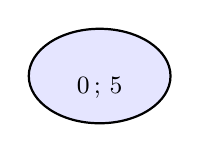
\begin{tikzpicture}[scale=0.75]
				\draw[thick, fill=blue!10] (0,0) ellipse (1.2cm and 0.8cm);
				\node at (0,0.3) {\textbf{$\N$}};
				\node[font=\small] at (0,-0.2) {$0 \,;\, 5$};
			\end{tikzpicture}
		\end{center}
	\end{wrapstuff}

	L'\textbf{ensemble des entiers naturels}, noté $\N$, est l'ensemble des entiers positifs ou nuls.
	\[
		\N = \{0\,;\, 1\,;\, 2\,;\, 3\,;\, 4\,;\, \dots\}
	\]
\end{df}

\begin{ex}
	$5 \in \N$ \quad et \quad $0 \in \N$.
\end{ex}

\subsection{L'ensemble des entiers relatifs $\Z$}

\begin{df}
	\nline
	\begin{wrapstuff}[r,width=4cm]
		\begin{center}
			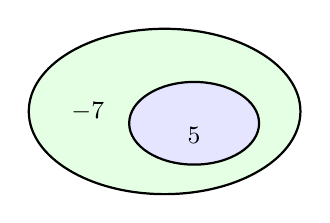
\begin{tikzpicture}[scale=0.75]
				\draw[thick, fill=green!10] (0,0) ellipse (2.3cm and 1.4cm);
				\node at (0,1) {\textbf{$\Z$}};
				\node[font=\small] at (-1.3,0) {$-7$};
				\draw[thick, fill=blue!10] (0.5,-0.2) ellipse (1.1cm and 0.7cm);
				\node at (0.5,0.05) {\textbf{$\N$}};
				\node[font=\small] at (0.5,-0.4) {$5$};
			\end{tikzpicture}
			\vspace*{-10mm}
		\end{center}
	\end{wrapstuff}
	L'\textbf{ensemble des entiers relatifs}, noté $\Z$, est l'ensemble des entiers positifs, négatifs ou nuls.
	\[
		\Z = \{\dots\,;\, - 3\,;\, - 2\,;\, - 1\,;\, 0\,;\, 1\,;\, 2\,;\, 3\,;\, \dots\}
	\]
\end{df}

\begin{ex}
	$-7 \in \Z$ \quad et \quad $5 \in \Z$ (tout entier naturel est aussi un entier relatif).
\end{ex}

\subsection{L'ensemble des nombres décimaux $\D$}

\begin{df}
	\nline
	\begin{wrapstuff}[r,width=5cm]
		\begin{center}
			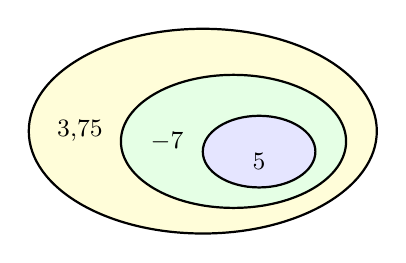
\begin{tikzpicture}[scale=0.65]
				\draw[thick, fill=yellow!15] (0,0) ellipse (3.4cm and 2cm);
				\node at (0,1.5) {\textbf{$\D$}};
				\node[font=\small] at (-2.4,0) {$3{,}75$};
				\draw[thick, fill=green!10] (0.6,-0.2) ellipse (2.2cm and 1.3cm);
				\node at (0.6,0.7) {\textbf{$\Z$}};
				\node[font=\small] at (-0.7,-0.2) {$-7$};
				\draw[thick, fill=blue!10] (1.1,-0.4) ellipse (1.1cm and 0.7cm);
				\node at (1.1,-0.15) {\textbf{$\N$}};
				\node[font=\small] at (1.1,-0.6) {$5$};
			\end{tikzpicture}
			\vspace*{-20mm}
		\end{center}
	\end{wrapstuff}

	L'\textbf{ensemble des nombres décimaux}, noté $\D$, est l'ensemble des nombres qui peuvent s'écrire sous la forme $\frac{a}{10^n}$, où $a \in \Z$ et $n \in \N$.

\end{df}

\begin{remarque}
	Un nombre décimal possède un \textbf{nombre fini de chiffres après la virgule}.
\end{remarque}

\begin{ex}
	$3{,}75 \in \D$ \quad car \quad $3{,}75 = \dfrac{375}{10^2}$
\end{ex}

\subsection{L'ensemble des nombres rationnels $\Q$}

\begin{df}
	\nline
	\begin{wrapstuff}[r,width=5.7cm]
		\begin{center}
			\begin{tikzpicture}[scale=0.55]
				\draw[thick, fill=orange!15] (0,0) ellipse (4.5cm and 2.6cm);
				\node at (0,2.1) {\textbf{$\Q$}};
				\node[font=\small] at (-3.2,0) {$\dfrac{1}{3}$};
				\draw[thick, fill=yellow!15] (0.7,-0.2) ellipse (3.3cm and 1.9cm);
				\node at (0.7,1.3) {\textbf{$\D$}};
				\node[font=\small] at (-1.7,-0.2) {$3{,}75$};
				\draw[thick, fill=green!10] (1.3,-0.4) ellipse (2.2cm and 1.2cm);
				\node at (1.3,0.4) {\textbf{$\Z$}};
				\node[font=\small] at (0,-0.4) {$-7$};
				\draw[thick, fill=blue!10] (1.8,-0.6) ellipse (1cm and 0.6cm);
				\node at (1.8,-0.35) {\textbf{$\N$}};
				\node[font=\small] at (1.8,-0.87) {$5$};
			\end{tikzpicture}
		\end{center}
		\vspace*{-10mm}
	\end{wrapstuff}

	L'\textbf{ensemble des nombres rationnels}, noté $\Q$, est l'ensemble des nombres qui peuvent s'écrire sous la forme d'une fraction $\frac{a}{b}$, avec $a \in \Z$ et $b \in \Z^*$ ($b \neq 0$).

	Son écriture décimale possède une \textbf{suite de chiffres qui se répète périodiquement} après la virgule.
\end{df}

\begin{ex}
	$\dfrac{1}{3} \in \Q$ \quad car \quad $\dfrac{1}{3} = 0{,}3333\dots$ (non décimal, mais rationnel ... voir démonstration ci-dessous).
\end{ex}

\begin{demo}[$\frac{1}{3}$ n'est pas un nombre décimal]
	On effectue un raisonnement par l'absurde.

	Supposons que $\tfrac{1}{3}$ soit un nombre décimal.

	Alors, par définition, il pourrait s'écrire sous la forme :

	\[
		\frac{1}{3} = \frac{a}{10^n} \quad \text{avec } a \in \Z \text{ et } n \in \N
	\]

	En effectuant le produit en croix, on obtient :

	\[
		3 \times a = 10^n \times 1 \implies 3a = 10^n
	\]

	Cela signifie que $10^n$ doit être un multiple de $3$.

	Or, un nombre est divisible par $3$ si la somme de ses chiffres est un multiple de $3$.

	La somme des chiffres de $10^n$ (qui s'écrit $1$ suivi de $n$ zéro(s)) est égale à $1 + 0 + \dots + 0 = 1$.

	Puisque $1$ n'est pas divisible par $3$, $10^n$ n'est jamais un multiple de $3$.

	Nous obtenons une \textbf{contradiction}.

	L'hypothèse de départ est donc fausse : $\frac{1}{3}$ n'est pas un nombre décimal $\pa{\frac{1}{3} \notin \D}$.
\end{demo}

\subsection{L'ensemble des nombres réels $\R$}

\begin{df}
	L'\textbf{ensemble des nombres réels}, noté $\R$, est l'ensemble de tous les nombres connus en Seconde (représentés par tous les points de la droite graduée).

	Il contient les nombres rationnels ainsi que les \textbf{nombres irrationnels}, qui ne peuvent pas s'écrire sous forme de fraction.
\end{df}

\begin{ex}
	$\sqrt{2} \in \R$ \quad et \quad $\pi \in \R$ \quad (ce sont des nombres irrationnels).
\end{ex}

\begin{demo}[$\sqrt{2}$ n'est pas un nombre rationnel]

	On effectue à nouveau un raisonnement par l'absurde.

	Supposons que $\sqrt{2}$ soit un nombre rationnel.

	Alors $\sqrt{2}$ s'écrit sous la forme d'une fraction irréductible :

	\[
		\sqrt{2} = \frac{a}{b} \quad \text{avec } a \in \N^*, b \in \N^*
	\]

	En élevant au carré des deux côtés :

	\[
		2 = \frac{a^2}{b^2} \implies a^2 = 2b^2
	\]

	Comme $a^2$ s'écrit sous la forme $2k$ (avec $k = b^2$), $a^2$ est un nombre \textbf{pair}.

	Or, le carré d'un nombre impair est impair. Ainsi, comme $a^2$ est pair, \textbf{$a$ est nécessairement pair}.

	Puisque $a$ est pair, il existe un entier $k \in \N^*$ tel que $a = 2k$.

	En remplaçant dans l'égalité $a^2 = 2b^2$ :

	\[
		(2k)^2 = 2b^2 \implies 4k^2 = 2b^2 \implies b^2 = 2k^2
	\]

	De même, $b^2$ s'écrit $2k^2$, donc $b^2$ est pair, ce qui implique que \textbf{$b$ est aussi pair}.

	Si $a$ et $b$ sont tous les deux pairs, ils sont tous les deux divisibles par $2$.

	Cela contredit le fait que $\dfrac{a}{b}$ est irréductible.

	Nous obtenons une \textbf{contradiction}.

	L'hypothèse de départ est donc fausse : $\sqrt{2}$ n'est pas un nombre rationnel ($\sqrt{2} \notin \Q$).
\end{demo}

\begin{prop}[Inclusion globale des ensembles de nombres]

	\[
		\N \subset \Z \subset \D \subset \Q \subset \R
	\]

\end{prop}

\begin{center}
	\begin{tikzpicture}[scale=0.95]
		\draw[thick, fill=red!10] (0,0) ellipse (5.8cm and 3.2cm);
		\node at (0,2.7) {\Large \textbf{$\R$}};
		\node[font=\small] at (-4.5,0.5) {$\pi$};
		\node[font=\small] at (-4.2,-0.8) {$\sqrt{2}$};
		\draw[thick, fill=orange!15] (0.8,-0.2) ellipse (4.5cm and 2.5cm);
		\node at (0.8,1.9) {\Large \textbf{$\Q$}};
		\node[font=\small] at (-2.5,0) {$\dfrac{1}{3}$};
		\draw[thick, fill=yellow!15] (1.5,-0.4) ellipse (3.4cm and 1.8cm);
		\node at (1.5,1.1) {\Large \textbf{$\D$}};
		\node[font=\small] at (-0.8,-0.4) {$3{,}75$};
		\draw[thick, fill=green!10] (2.1,-0.6) ellipse (2.3cm and 1.2cm);
		\node at (2.1,0.2) {\Large \textbf{$\Z$}};
		\node[font=\small] at (0.7,-0.6) {$-7$};
		\draw[thick, fill=blue!10] (2.7,-0.8) ellipse (1.2cm and 0.6cm);
		\node at (2.7,-0.55) {\Large \textbf{$\N$}};
		\node[font=\small] at (2.7,-0.95) {$5$};
	\end{tikzpicture}
\end{center}

\begin{ex}
	\nline
	\begin{enumerate}
		\item \textbf{Étude de $A = \dfrac{7}{6} - \dfrac{5}{4} + \dfrac{1}{12}$ :}

		      On met tout au même dénominateur :

		      \[
			      A = \frac{7 \times 2}{6 \times 2} - \frac{5 \times 3}{4 \times 3} + \frac{1}{12} = \frac{14 - 15 + 1}{12} = \frac{0}{12} = 0
		      \]

		      Malgré les fractions, le résultat final est $0$.

		      On a donc : $A \in \N$ (et par inclusion $A \in \Z, \D, \Q, \R$).

		\item \textbf{Étude de $B = \dfrac{147}{63}$ :}

		      On décompose le numérateur et le dénominateur en facteurs premiers :

		      \[
			      B = \frac{3 \times 7^2}{3^2 \times 7} = \frac{7}{3} = 2{,}3333\dots
		      \]

		      La fraction est irréductible et son dénominateur ($3$) contient un facteur autre que $2$ et $5$.

		      On a donc : $B \notin \D$, mais $B \in \Q$ et $B \in \R$.

		\item \textbf{Calcul avec des puissances :}

		      \[
			      C = \frac{3^2 \times 5}{10^2} = \frac{9 \times 5}{100} = \frac{45}{100} = 0{,}45
		      \]

		      Le nombre s'écrit sous la forme $\dfrac{45}{10^2}$, il possède un nombre fini de chiffres après la virgule.

		      Donc $C \in \D$ (et $C \in \Q, \R$), mais $C \notin \Z$.

		\item \textbf{Simplification d'un quotient avec racine carrée :}

		      \[
			      D = \frac{\sqrt{50}}{\sqrt{2}} = \sqrt{\frac{50}{2}} = \sqrt{25} = 5
		      \]

		      Après calcul, le résultat est un entier naturel : $A \in \N$ (et donc $A \in \Z, \D, \Q, \R$).

	\end{enumerate}
\end{ex}

\begin{remarque}[Subtilités de notation]
	\nline
	\begin{itemize}
		\item \textbf{L'exclusion du zéro :}

		      Un astérisque en exposant signifie que l'on exclut le nombre $0$.

		      \begin{itemize}
			      \item $\R^* = \R \setminus \{0\}$ est l'ensemble des réels non nuls ($x \neq 0$).
			      \item $\N^* = \{1\,;\, 2\,;\, 3\,;\, \dots\}$ est l'ensemble des entiers naturels non nuls.
		      \end{itemize}

		\item \textbf{La restriction de signe ($+$ et $-$) :}

		      L'ajout d'un signe en indice indique qu'on ne conserve que les nombres positifs ou négatifs.

		      \begin{itemize}
			      \item $\R^+$ est l'ensemble des réels positifs ou nuls ($x \geqslant 0$).
			      \item $\R^-$ est l'ensemble des réels négatifs ou nuls ($x \leqslant 0$).
			      \item $\R^*_+$ est l'ensemble des réels strictement positifs ($x > 0$).
		      \end{itemize}
	\end{itemize}
\end{remarque}

\section{Intervalles de $\R$}

\subsection{Définition d'un intervalle}

\begin{df}
	Un \textbf{intervalle} de $\R$ est une partie de la droite numérique formée de tous les réels compris entre deux bornes $a$ et $b$ (avec $a \leqslant b$), ou s'étendant sans limite d'un côté (notion d'infini $\infty$).

	\begin{itemize}
		\item Si les bornes $a$ et $b$ sont incluses, l'intervalle est dit \textbf{fermé} : $\intff{a}{b}$.
		\item Si les bornes $a$ et $b$ sont exclues, l'intervalle est dit \textbf{ouvert} : $\intoo{a}{b}$.
		\item Si $a$ est inclus et $b$ est exclu, l'intervalle est \textbf{fermé en $a$ et ouvert en $b$} : $\intfo{a}{b}$.
		\item Si $a$ est exclu et $b$ est inclus, l'intervalle est \textbf{ouvert en $a$ et fermé en $b$} : $\intof{a}{b}$.
	\end{itemize}
\end{df}

\begin{ex}
	L'ensemble des réels $x$ vérifiant $2 \leqslant x \leqslant 5$ est l'intervalle fermé $\intff{2}{5}$.

	Il contient tous les nombres compris entre $2$ et $5$, y compris $2$ et $5$.

	% --- Représentation graphique TikZ de l'exemple ---
	\begin{center}
		\begin{tikzpicture}[scale=1.9]
			% Axe gradué avec ton style de flèche
			\draw[->, very thick] (-0.5,0) -- (5.5,0);
			\foreach \x in {0, 1, 2, 3, 4, 5} { \draw[thick] (\x,0.1) -- (\x,-0.1) node[below=1mm] {$\x$}; }
			\draw[blue, line width=2pt, {Bracket[length=4pt, width=15pt]}-{Bracket[length=4pt, width=15pt]}] (1.99,0) -- (5.01,0);
			\node[blue, above=5pt] at (3.5,0) {\Large $\intff{2}{5}$};
		\end{tikzpicture}
	\end{center}
\end{ex}

\begin{ex}
	\nline
	\begin{enumerate}
		\item \textbf{Intervalle fermé} \qquad $x\in\intff{1}{4}\quad\iff\quad 1 \leqslant x \leqslant 4$
		      \ms
		      \begin{center}
			      \begin{tikzpicture}[scale=1]
				      \draw[->, thick] (-0.5,0) -- (5.5,0);
				      \foreach \x in {0, 1, 2, 3, 4, 5} { \draw[thick] (\x,0.08) -- (\x,-0.08) node[below=1mm] {$\x$}; }
				      \draw[blue, line width=2pt, {Bracket[length=4pt, width=15pt]}-{Bracket[length=4pt, width=15pt]}] (0.95,0) -- (4.05,0);
				      \node[blue, above=3pt] at (2.5,0) {$\intff{1}{4}$};
			      \end{tikzpicture}
		      \end{center}
		      \ms
		\item \textbf{Intervalle ouvert}\qquad $x\in\intoo{1}{4}\quad\iff\quad 1 < x < 4$
		      \ms
		      \begin{center}
			      \begin{tikzpicture}[scale=1]
				      \draw[->, thick] (-0.5,0) -- (5.5,0);
				      \foreach \x in {0, 1, 2, 3, 4, 5} { \draw[thick] (\x,0.08) -- (\x,-0.08) node[below=1mm] {$\x$}; }
				      \draw[blue, line width=2pt, {Bracket[length=4pt, width=15pt, reversed]}-{Bracket[length=4pt, width=15pt, reversed]}] (0.85,0) -- (4.15,0);
				      \node[blue, above=3pt] at (2.5,0) {$\intoo{1}{4}$};
			      \end{tikzpicture}
		      \end{center}
		      \ms
		\item \textbf{Intervalle fermé en $1$ et ouvert en $4$} \qquad $x\in\intfo{1}{4}\quad\iff\quad 1 \leqslant x < 4$
		      \ms
		      \begin{center}
			      \begin{tikzpicture}[scale=1]
				      \draw[->, thick] (-0.5,0) -- (5.5,0);
				      \foreach \x in {0, 1, 2, 3, 4, 5} { \draw[thick] (\x,0.08) -- (\x,-0.08) node[below=1mm] {$\x$}; }
				      \draw[blue, line width=2pt, {Bracket[length=4pt, width=15pt]}-{Bracket[length=4pt, width=15pt, reversed]}] (0.95,0) -- (4.15,0);
				      \node[blue, above=3pt] at (2.5,0) {$\intfo{1}{4}$};
			      \end{tikzpicture}
		      \end{center}
		      \ms
		\item \textbf{Intervalle ouvert en $1$ et fermé en $4$} \qquad $x\in \intof{1}{4}\quad\iff\quad 1 < x \leqslant 4$
		      \ms
		      \begin{center}
			      \begin{tikzpicture}[scale=1]
				      \draw[->, thick] (-0.5,0) -- (5.5,0);
				      \foreach \x in {0, 1, 2, 3, 4, 5} { \draw[thick] (\x,0.08) -- (\x,-0.08) node[below=1mm] {$\x$}; }
				      \draw[blue, line width=2pt, {Bracket[length=4pt, width=15pt, reversed]}-{Bracket[length=4pt, width=15pt]}] (0.85,0) -- (4.05,0);
				      \node[blue, above=3pt] at (2.5,0) {$\intof{1}{4}$};
			      \end{tikzpicture}
		      \end{center}
	\end{enumerate}
\end{ex}
\ms
\begin{remarque}[L'infini ($\infty$)]
	\nline
	\begin{itemize}
		\item \textbf{L'infini n'est pas un nombre :} Les symboles $+\infty$ (\og{}plus l'infini\fg{}) et $-\infty$ (\og{}moins l'infini\fg{}) ne désignent pas des nombres réels, mais indiquent que l'intervalle s'étend sans limite vers la droite ou vers la gauche.

		\item \textbf{On exclut TOUJOURS l'infini :} Comme l'infini n'est pas un nombre, on ne peut jamais l'atteindre ni le contenir dans un intervalle. Le crochet du côté de $+\infty$ ou $-\infty$ est donc \textbf{toujours ouvert}.
		      \begin{itemize}
			      \item \textbf{Intervalle \og{}limité uniquement à gauche\fg{} :}

			            L'ensemble des réels $x$ supérieurs ou égaux à $3$ s'écrit :

			            \[
				            x \geqslant 3 \iff x \in \intfo{3}{+\infty}
			            \]

			            \begin{center}
				            \begin{tikzpicture}[scale=1]
					            % Axe gradué
					            \draw[->, thick] (-1,0) -- (6,0);
					            \foreach \x in {0, 1, 2, 3, 4, 5} {
							            \draw[thick] (\x,0.08) -- (\x,-0.08) node[below=1mm] {\small $\x$};
						            }
					            % Demi-droite [3; +infty[
					            \draw[blue, line width=2pt, {Bracket[length=4pt, width=15pt]}-] (2.95,0) -- (5.8,0);
					            \node[blue, above=3pt] at (4.4,0) {$\intfo{3}{+\infty}$};
				            \end{tikzpicture}
			            \end{center}

			      \item \textbf{Intervalle \og{}limité uniquement à droite\fg{} :}

			            L'ensemble des réels $x$ strictement inférieurs à $-1$ s'écrit :

			            \[
				            x < -1 \iff x \in \intoo{-\infty}{-1}
			            \]

			            \begin{center}
				            \begin{tikzpicture}[scale=1]
					            % Axe gradué
					            \draw[->, thick] (-3,0) -- (3,0);
					            \foreach \x in {-2, -1, 0, 1, 2} {
							            \draw[thick] (\x,0.08) -- (\x,-0.08) node[below=1mm] {\small $\x$};
						            }
					            % Demi-droite ]-infty; -1[
					            \draw[blue, line width=2pt, -{Bracket[length=4pt, width=15pt, reversed]}] (-3.4,0) -- (-0.85,0);
					            \node[blue, above=3pt] at (-1.9,0) {$\intoo{-\infty}{-1}$};
				            \end{tikzpicture}
			            \end{center}

		      \end{itemize}
		\item \textbf{L'ensemble $\R$ tout entier :} La droite numérique s'étend de $-\infty$ à $+\infty$ sans interruption.

		      On peut donc écrire l'ensemble des nombres réels sous forme d'un unique intervalle :

		      \[
			      \R = \intoo{-\infty}{+\infty}
		      \]

	\end{itemize}
\end{remarque}

\subsection{Appartenance d'un nombre à un intervalle}

\begin{meth}
	Pour déterminer si un nombre appartient à un intervalle, on traduit la condition d'appartenance $\in$ par des inégalités (ou un calcul direct) et on vérifie si la borne est ouverte ou fermée.

	\begin{itemize}
		\item $3 \in \intff{2}{5}$ \quad car \quad $2 \leqslant 3 \leqslant 5$.
		\item $2 \in \intff{2}{5}$ \quad car l'intervalle est fermé en $2$ (le crochet \og{}inclut\fg{} le $2$).
		\item $2 \notin \intof{2}{5}$ \quad car l'intervalle est ouvert en $2$ (le crochet \og{}exclut\fg{} le $2$).
		\item $-1 \notin \intff{2}{5}$ \quad car $-1 < 2$.
		\item $\pi \in \intff{2}{5}$ \quad car $\pi \approx 3{,}14$ et $2 \leqslant 3{,}14 \leqslant 5$.
	\end{itemize}
\end{meth}

\begin{ex}
	\textbf{Exemples d'appartenance après calcul :}

	\begin{enumerate}
		\item \textbf{Étude de $\mathbf{\frac{13}{4}}$ vis-à-vis de $\intfo{3}{+\infty}$ :} \quad $\frac{13}{4} = 3{,}25 \quad \text{et} \quad 3{,}25 \geqslant 3$

		      On a donc $\dfrac{13}{4} \in \intfo{3}{+\infty}$.

		\item \textbf{Étude de $\mathbf{\frac{-7}{3}}$ vis-à-vis de $\intoo{-\infty}{-2}$ :} \quad $\frac{-7}{3} \approx -2{,}33 \quad \text{et} \quad -2{,}33 < -2$

		      On a donc $\dfrac{-7}{3} \in \intoo{-\infty}{-2}$.

		\item \textbf{Étude de $\mathbf{\sqrt{3}}$ vis-à-vis de $\intff{1}{2}$ :}

		      Comme $1 < 3 < 4$, on passe à la racine carrée : \quad $\sqrt{1} < \sqrt{3} < \sqrt{4} \implies 1 < \sqrt{3} < 2$

		      On a donc $\sqrt{3} \in \intff{1}{2}$.
	\end{enumerate}
\end{ex}

\subsection{Union et intersection d'intervalles}

\begin{df}
	Soient $I$ et $J$ deux intervalles de $\R$.
	\begin{itemize}
		\item \textbf{L'intersection} de $I$ et $J$, notée $I \cap J$ (se lit \og{}$I$ inter $J$\fg{}), est l'ensemble des réels $x$ qui appartiennent \textbf{à la fois} à $I$ \textbf{et} à $J$.
		      \[
			      x \in I \cap J \iff x \in I \quad \text{\textbf{et}} \quad x \in J
		      \]
		\item \textbf{L'union} (ou réunion) de $I$ et $J$, notée $I \cup J$ (se lit \og{}$I$ union $J$\fg{}), est l'ensemble des réels $x$ qui appartiennent à $I$ \textbf{ou} à $J$ (au moins à l'un des deux).
		      \[
			      x \in I \cup J \iff x \in I \quad \text{\textbf{ou}} \quad x \in J
		      \]
	\end{itemize}
\end{df}

\begin{prop}
	\nline
	\begin{enumerate}
		\item Si un élément appartient à l'intersection $I \cap J$, alors il appartient nécessairement à l'union $I \cup J$.
		\item Si deux intervalles \textbf{n'ont aucun nombre en commun}, leur intersection est l'ensemble vide, noté $\emptyset$ :
		      \[
			      I \cap J = \emptyset
		      \]
	\end{enumerate}
\end{prop}

\begin{ex}

	Considérons les intervalles $I = \intff{-1}{3}$ et $J = \intfo{1}{5}$.

	Déterminons graphiquement $I \cap J$ et $I \cup J$.

	\begin{center}
		\begin{tikzpicture}[scale=1]
			% Graduation commune
			\foreach \x in {-2, -1, 0, 1, 2, 3, 4, 5, 6} {
					\draw[gray!40, dashed] (\x,-2.8) -- (\x,0.8);
					\node[below] at (\x,-2.8) {\small $\x$};
				}

			% Axe 1 : Intervalle I = [-1 ; 3]
			\draw[->, thick] (-2.5,0.5) -- (6.5,0.5);
			\draw[blue, line width=2pt, {Bracket[length=4pt, width=15pt]}-{Bracket[length=4pt, width=15pt]}] (-1,0.5) -- (3,0.5);
			\node[blue, left] at (-2.5,0.5) {$I = \intff{-1}{3}$};

			% Axe 2 : Intervalle J = [1 ; 5[
			\draw[->, thick] (-2.5,-0.5) -- (6.5,-0.5);
			\draw[red!80!black, line width=2pt, {Bracket[length=4pt, width=15pt]}-{Bracket[length=4pt, width=15pt, reversed]}] (1,-0.5) -- (5.1,-0.5);
			\node[red!80!black, left] at (-2.5,-0.5) {$J = \intfo{1}{5}$};

			% Axe 3 : Intersection I \cap J
			\draw[->, thick] (-2.5,-1.5) -- (6.5,-1.5);
			\draw[purple, line width=2.5pt, {Bracket[length=4pt, width=15pt]}-{Bracket[length=4pt, width=15pt]}] (1,-1.5) -- (3,-1.5);
			\node[purple, left] at (-2.5,-1.5) {$I \cap J = \intff{1}{3}$};

			% Axe 4 : Union I \cup J
			\draw[->, thick] (-2.5,-2.5) -- (6.5,-2.5);
			\draw[green!50!black, line width=2.5pt, {Bracket[length=4pt, width=15pt]}-{Bracket[length=4pt, width=15pt, reversed]}] (-1,-2.5) -- (5.1,-2.5);
			\node[green!50!black, left] at (-2.5,-2.5) {$I \cup J = \intfo{-1}{5}$};
		\end{tikzpicture}
	\end{center}

	\begin{itemize}
		\item \textbf{Intersection :} La zone où les deux couleurs se superposent donne $I \cap J = \intff{1}{3}$.
		\item \textbf{Union :} La zone couverte par au moins l'une des deux couleurs donne $I \cup J = \intfo{-1}{5}$.
	\end{itemize}
\end{ex}

\begin{ex}{Cas particuliers : Intervalles disjoints}
	Considérons les intervalles $K = \intff{-1}{0}$ et $L = \intff{3}{4}$.

	\begin{center}
		\begin{tikzpicture}[scale=1]
			\draw[->, thick] (-2,0) -- (5,0);
			\foreach \x in {-1, 0, 1, 2, 3, 4} { \draw[thick] (\x,0.08) -- (\x,-0.08) node[below=1mm] {\small $\x$}; }
			\draw[blue, line width=2pt, {Bracket[length=4pt, width=15pt]}-{Bracket[length=4pt, width=15pt]}] (-1.05,0) -- (0.05,0);
			\node[blue, above=3pt] at (-0.5,0) {$K$};
			\draw[red!80!black, line width=2pt, {Bracket[length=4pt, width=15pt]}-{Bracket[length=4pt, width=15pt]}] (2.95,0) -- (4.05,0);
			\node[red!80!black, above=3pt] at (3.5,0) {$L$};
		\end{tikzpicture}
	\end{center}

	\begin{enumerate}
		\item \textbf{Intersection nulle (vide) :}
		      Les intervalles $K$ et $L$ n'ont aucun nombre en commun. On écrit :
		      \[
			      K \cap L = \emptyset
		      \]
		\item \textbf{Union non simplifiable :}
		      Comme il y a un \og{}trou\fg{} entre $0$ et $3$, la réunion ne peut pas s'écrire sous la forme d'un seul intervalle. L'expression reste donc sous la forme :
		      \[
			      K \cup L = \intff{-1}{0} \cup \intff{3}{4}
		      \]
	\end{enumerate}
\end{ex}

\section{Valeur absolue et distance}

\subsection{Définition et premières propriétés}

\begin{df}
	Soit $x$ un nombre réel. On appelle \textbf{valeur absolue} de $x$, notée $\abs{x}$, le nombre réel positif ou nul défini par :
	\[
		\abs{x} =
		\begin{cases}
			x  & \text{si } x \geqslant 0 \\
			-x & \text{si } x < 0
		\end{cases}
	\]
\end{df}

\begin{prop}
	Pour tout réel $x$ :
	\begin{itemize}
		\item $\abs{x} \geqslant 0$ (la valeur absolue est toujours positive ou nulle).
		\item $\abs{-x} = \abs{x}$.
		\item $\abs{x} = 0 \iff x = 0$.
	\end{itemize}
\end{prop}

\begin{ex}
	\nline
	\begin{itemize}
		\item $\abs{3} = 3$ car $3 \geqslant 0$.
		\item $\abs{-5} = -(-5) = 5$ car $-5 < 0$.
		\item $\abs{\pi - 5} = -(\pi - 5) = 5 - \pi$ car $\pi - 5 < 0$.
	\end{itemize}
\end{ex}

\subsection{Distance entre deux réels}

\begin{df}
	Soient $a$ et $b$ deux réels, repérés par les points $A$ et $B$ sur une droite graduée.

	La \textbf{distance} entre $a$ et $b$, notée $d(a,b)$, est égale à la longueur du segment $[AB]$ :
	\[
		d(a,b) = \abs{b - a} = \abs{a - b}
	\]

	\begin{center}
		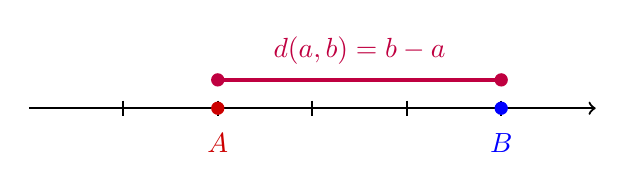
\begin{tikzpicture}[scale=1.2]
			\draw[->, thick] (-1,0) -- (5,0);
			\foreach \x in {0,1,2,3,4} { \draw[thick] (\x,0.08) -- (\x,-0.08); }
			\fill[red!80!black] (1,0) circle (2pt) node[below=2mm] {$A$};
			\fill[blue] (4,0) circle (2pt) node[below=2mm] {$B$};
			\fill[purple] (1,0.3) circle (2pt);
			\fill[purple] (4,0.3) circle (2pt);
			\draw[line width=1.5pt, purple] (1,0.3) -- (4,0.3);
			\node[purple, above=2pt] at (2.5,0.3) {$d(a,b) = \abs{b - a}$};
		\end{tikzpicture}
	\end{center}
\end{df}

\begin{remarque}
	En particulier, pour tout réel $x$, la valeur absolue $\abs{x} = \abs{x - 0} = d(x,0)$ représente la \textbf{distance entre $x$ et l'origine $0$}.
\end{remarque}

\subsection{Équations et inéquations avec valeur absolue}

\begin{prop}[Résolution d'équations $\abs{x - a} = r$]
	Soient $a \in \R$ et $r \geqslant 0$.

	L'équation $\abs{x - a} = r$ signifie que la distance entre $x$ et $a$ est égale à $r$.
	\[
		\abs{x - a} = r \iff \begin{cases}x_1 = a - r \\ x_2 = a + r\end{cases}
	\]
\end{prop}

\begin{ex}
	Résolvons dans $\R$ l'équation $\abs{x - 2} = 3$.

	On cherche les réels $x$ situés à une distance de $3$ du point d'abscisse $2$.

	\begin{center}
		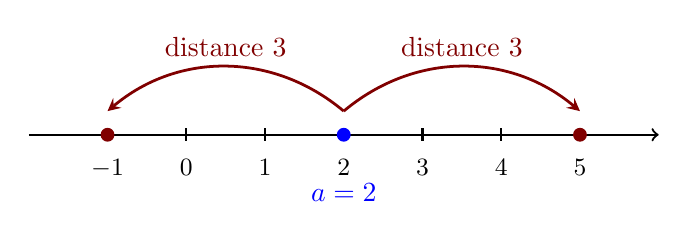
\begin{tikzpicture}[scale=1]
			\draw[->, thick] (-2,0) -- (6,0);
			\foreach \x in {-1,0,1,2,3,4,5} { \draw[thick] (\x,0.08) -- (\x,-0.08) node[below=1mm] {\small $\x$}; }
			\fill[blue] (2,0) circle (2.5pt) node[below=5mm] {$a = 2$};
			\draw[->, >=stealth, line width=1pt, red!50!black] (2,0.3) to[out=140,in=40] node[midway,above] {distance $3$} (-1,0.3);
			\draw[->, >=stealth, line width=1pt, red!50!black] (2,0.3) to[out=40,in=140] node[midway,above] {distance $3$} (5,0.3);
			\fill[red!50!black] (-1,0) circle (2.5pt);
			\fill[red!50!black] (5,0) circle (2.5pt);
		\end{tikzpicture}
	\end{center}

	L'ensemble des solutions est $S = \{-1 \,;\, 5\}$.
\end{ex}

\begin{prop}[Résolution d'inéquations $\abs{x - a} \leqslant r$]
	Soient $a \in \R$ et $r \geqslant 0$.

	L'inéquation $\abs{x - a} \leqslant r$ signifie que la distance entre $x$ et $a$ est inférieure ou égale à $r$.
	\begin{align*}
		\abs{x - a} \leqslant r & \iff x \in \intff{\pa{a - r}}{\pa{a + r}}        \\
		                        & \iff \pa{a - r} \leqslant x \leqslant \pa{a + r}
	\end{align*}
\end{prop}

\begin{ex}
	Résolvons dans $\R$ l'inéquation $\abs{x - 2} \leqslant 3$.

	\textbf{Interprétation :} On cherche les réels $x$ dont la distance à $2$ est inférieure ou égale à $3$.

	\begin{center}
		\begin{tikzpicture}[scale=1]
			% Axe
			\draw[->, thick] (-2.5,0) -- (6.5,0);
			\foreach \x in {-2,-1,0,1,3,4,5,6} { \draw[thick] (\x,0.08) -- (\x,-0.08) node[below=1mm] {\small $\x$}; }

			% Intervalle solution
			\draw[blue, line width=1.5pt, {Bracket[length=4pt, width=13pt]}-{Bracket[length=4pt, width=13pt]}] (-1.03,0) -- (5.03,0);
			\node[blue, above=6pt] at (2,0) {$\intff{-1}{5}$};
			\fill (2,0) circle (2pt) node[below=2mm] {$a = 2$};

			% Flèches de rayon
			\draw[<->, >=stealth, thick, red!50!black] (-1,-1) -- (2,-1) node[midway,below] {$r=3$};
			\draw[<->, >=stealth, thick, red!50!black] (2,-1) -- (5,-1) node[midway,below] {$r=3$};
		\end{tikzpicture}
	\end{center}

	L'ensemble des solutions est l'intervalle $S = \intff{-1}{5}$.
\end{ex}



% \input{tex/2nde/equations-inequations}
% \part{Statistiques et probabilités}
% \input{tex/2nde/proportion}
% \chapter{Statistiques descriptives}

\section{Vocabulaire et présentation d'une série}

\begin{defin}[Vocabulaire de base]
	\textbf{Population et individu :} L'ensemble étudié en statistiques est appelé la \textbf{population}. Chaque élément qui constitue cet ensemble est un \textbf{individu}.

	\textbf{Caractère :} C'est la propriété ou la grandeur étudiée sur chaque individu.
	\begin{itemize}
		\item Un caractère est dit \textbf{qualitatif} lorsque ses valeurs (appelées modalités) ne sont pas des nombres (ex. : couleur des yeux, filière).
		\item Un caractère est dit \textbf{quantitatif} lorsqu'il prend des valeurs numériques.
		      \begin{itemize}
			      \item Il est \textbf{discret} si les valeurs sont \og{}isolées\fg{} (ex. : nombre d'enfants)
			      \item Il est \textbf{continu} si les valeurs sont regroupées en intervalles appelés \textbf{classes} (ex. : taille en $\text{cm}$)
		      \end{itemize}
	\end{itemize}
\end{defin}

\begin{defin}[Effectifs, fréquences et cumul]
	Soit une série statistique de $k$ valeurs distinctes $x_1, x_2, \dots, x_k$ (ordonnées dans l'ordre croissant).
	\begin{itemize}
		\item L'\textbf{effectif} $n_i$ associé à la valeur $x_i$ est le nombre d'individus possédant cette valeur.
		\item L'\textbf{effectif total} est la somme de tous les effectifs :
		      \[
			      N = n_1 + n_2 + \dots + n_k \qquad = \displaystyle\sum_{i=1}^k n_i
		      \]
		\item La \textbf{fréquence} $f_i$ associée à la valeur $x_i$ est le quotient $f_i = \dfrac{n_i}{N}$. La somme des fréquences est égale à $1$ (ou $100\,\%$).
		\item L'\textbf{effectif cumulé croissant (E.C.C.)} associé à la valeur $x_i$ est la somme des effectifs de toutes les valeurs inférieures ou égales à $x_i$.
		\item La \textbf{fréquence cumulée croissante (F.C.C.)} associée à la valeur $x_i$ est la somme des fréquences de toutes les valeurs inférieures ou égales à $x_i$.
	\end{itemize}
\end{defin}

\begin{ex}[Présentation des données sous forme de tableau]
	Voici une série de notes obtenues par un groupe d'élèves :

	\[
		4 \ ; \ 6 \ ; \ 7 \ ; \ 12 \ ; \ 12 \ ; \ 17 \ ; \ 18 \ ; \ 18
	\]

	L'effectif total est $N = 8$.

	\begin{center}
		\rnc{\arraystretch}{1.5}
		\begin{tabular}{|r|c|c|c|c|c|c|}
			\hline
			\rowcolor{gray!30}Notes $x_i$          & 4              & 6              & 7              & 12             & 17             & 18             \\ \hline
			Effectifs $n_i$                        & 1              & 1              & 1              & 2              & 1              & 2              \\ \hline
			E.C.C.                                 & 1              & 2              & 3              & 5              & 6              & 8              \\ \hline
			\rule[-4mm]{0mm}{11mm}Fréquences $f_i$ & $\dfrac{1}{8}$ & $\dfrac{1}{8}$ & $\dfrac{1}{8}$ & $\dfrac{2}{8}$ & $\dfrac{1}{8}$ & $\dfrac{2}{8}$ \\ \hline
			\rule[-4mm]{0mm}{11mm}F.C.C.           & $\dfrac{1}{8}$ & $\dfrac{2}{8}$ & $\dfrac{3}{8}$ & $\dfrac{5}{8}$ & $\dfrac{6}{8}$ & $\dfrac{8}{8}$ \\ \hline
		\end{tabular}
	\end{center}
\end{ex}

\section{Caractéristiques de position}

Les caractéristiques de position (ou de tendance centrale) résument une série statistique par une valeur numérique représentative.

\subsection{Moyenne}

\begin{defin}[Moyenne pondérée]
	La \textbf{moyenne} d'une série statistique de valeurs $x_1, x_2, \dots, x_k$ affectées des effectifs $n_1, n_2, \dots, n_k$ est notée $\bar{x}$. Elle est définie par :

	\[
		\bar{x} = \dfrac{n_1 x_1 + n_2 x_2 + \dots + n_k x_k}{N} \qquad = \dfrac{1}{N} \sum_{i=1}^k n_i x_i
	\]

	Dans le cas d'un caractère continu regroupé en classes $[a ; b[$, on effectue le calcul en remplaçant chaque classe par son centre $\dfrac{a+b}{2}$.
\end{defin}

\begin{ex}[Calcul d'une moyenne simple et pondérée]
	On étudie le nombre de frères et sœurs des $21$ élèves d'une classe de 1STMG :
	\[
		0 \ ; \ 0 \ ; \ 0 \ ; \ 0 \ ; \ 0 \ ; \ 1 \ ; \ 1 \ ; \ 1 \ ; \ 1 \ ; \ 1 \ ; \ 1 \ ; \ 1 \ ; \ 1 \ ; \ 2 \ ; \ 2 \ ; \ 2 \ ; \ 2 \ ; \ 3 \ ; \ 3 \ ; \ 3 \ ; \ 4
	\]

	\begin{enumerate}
		\item \textbf{Calcul non pondéré (moyenne simple) :}

		      On additionne directement l'ensemble des $21$ valeurs individuelles :
		      \[
			      \bar{x} = \dfrac{0 + 0 + 0 + 0 + 0 + 1 + 1 + 1 + 1 + 1 + 1 + 1 + 1 + 2 + 2 + 2 + 2 + 3 + 3 + 3 + 4}{21} = \dfrac{29}{21} \approx 1{,}38
		      \]

		\item \textbf{Calcul pondéré (à partir du tableau d'effectifs) :}

		      En regroupant les valeurs identiques avec leur effectif $n_i$ associé :
		      \begin{center}
			      \rnc{\arraystretch}{1.3}
			      \begin{tabular}{|r|c|c|c|c|c|} \hline
				      \rowcolor{gray!30} Nombre de frères et sœurs $x_i$ & 0 & 1 & 2 & 3 & 4 \\ \hline
				      Effectifs $n_i$                                    & 5 & 8 & 4 & 3 & 1 \\ \hline
			      \end{tabular}
		      \end{center}

		      Le calcul devient :
		      \[
			      \bar{x} = \dfrac{5 \times 0 + 8 \times 1 + 4 \times 2 + 3 \times 3 + 1 \times 4}{21} = \dfrac{29}{21} \approx 1{,}38
		      \]
	\end{enumerate}

	On vérifie bien que les deux méthodes mènent au même résultat.
\end{ex}

\begin{ex}[Calcul de la moyenne d'un caractère continu]
	Dans une classe de 1STMG, on mesure la taille des élèves (en $\text{cm}$) regroupée par classes d'amplitude $5\text{ cm}$ :

	\begin{center}
		\rnc{\arraystretch}{1.3}
		\begin{tabular}{|c|c|c|c|}\hline
			\rowcolor{gray!30}
			Taille $I_i$ (en $\text{cm}$) & Centre $c_i$ & Effectif $n_i$ & $n_i \times c_i$              \\ \hline
			$[160 ; 165[$                 & $162{,}5$    & 4              & $4 \times 162{,}5 = 650$      \\ \hline
			$[165 ; 170[$                 & $167{,}5$    & 9              & $9 \times 167{,}5 = 1507{,}5$ \\ \hline
			$[170 ; 175[$                 & $172{,}5$    & 8              & $8 \times 172{,}5 = 1380$     \\ \hline
			$[175 ; 180[$                 & $177{,}5$    & 3              & $3 \times 177{,}5 = 532{,}5$  \\ \hline
			\textbf{Total}                & -            & $N = 24$       & $4070$                        \\ \hline
		\end{tabular}
	\end{center}

	On calcule la taille moyenne estimée en appliquant la formule de la moyenne pondérée aux centres des classes :
	\[
		\bar{x} = \dfrac{4 \times 162{,}5 + 9 \times 167{,}5 + 8 \times 172{,}5 + 3 \times 177{,}5}{24} = \dfrac{4070}{24} \approx 169{,}58\text{ cm}
	\]
\end{ex}

\newpage

\begin{prop}[Linéarité de la moyenne]
	Soit une série de moyenne $\bar{x}$ et deux réels $a$ et $b$.
	\begin{itemize}
		\item Si on multiplie toutes les valeurs de la série par $a$, la nouvelle moyenne devient $a\bar{x}$.
		\item Si on ajoute $b$ à toutes les valeurs de la série, la nouvelle moyenne devient $\bar{x} + b$.
		\item De façon générale, les valeurs $a x_i + b$ ont pour moyenne $a\bar{x} + b$.
	\end{itemize}
\end{prop}

\begin{methode}[Utiliser la linéarité de la moyenne]
	Un relevé du prix au litre d'essence dans 5 stations donne :
	\[
		1{,}50\text{ \euro}, 1{,}44\text{ \euro}, 1{,}51\text{ \euro}, 1{,}62\text{ \euro} \text{ et } 1{,}58\text{ \euro}
	\]

	\begin{enumerate}
		\item Calculer le prix moyen initial.
		\item Calculer le prix moyen après une augmentation générale de $30\,\%$.
		\item Calculer le prix moyen final après une remise de $0{,}15\text{ \euro}$ par litre.
	\end{enumerate}

	\begin{correction}
		\nline
		\begin{enumerate}
			\item Prix moyen initial : $\bar{x} = \dfrac{1{,}50 + 1{,}44 + 1{,}51 + 1{,}62 + 1{,}58}{5} = \dfrac{7{,}65}{5} = 1{,}53\text{ \euro}$.
			\item Augmenter de $30\,\%$ revient à multiplier par $1{,}30$. Par linéarité :
			      \[
				      \bar{x}_{\text{hausse}} = 1{,}53 \times 1{,}30 = 1{,}989\text{ \euro}
			      \]

			\item Soustraire $0{,}15\text{ \euro}$ à chaque valeur revient à soustraire $0{,}15$ à la moyenne :
			      \[
				      \bar{x}_{\text{final}} = 1{,}989 - 0{,}15 = 1{,}839\text{ \euro}
			      \]
		\end{enumerate}
	\end{correction}
\end{methode}

\subsection{Médiane}

\begin{defin}[Médiane]
	La \textbf{médiane} d'une série ordonnée dans l'ordre croissant, notée $M_e$, est une valeur qui partage la série en deux groupes de même effectif :
	\begin{itemize}
		\item Au moins $50\,\%$ des valeurs sont inférieures ou égales à $M_e$, ...
		\item ... et au moins $50\,\%$ des valeurs sont supérieures ou égales à $M_e$.
	\end{itemize}
\end{defin}

\begin{methode}[Déterminer la médiane d'une série discrète]
	Soit $N$ l'effectif total de la série rangée dans l'ordre croissant.
	\begin{itemize}
		\item \textbf{Si $N$ est impair ($N = 2p + 1$) :} la médiane est la valeur de rang $p + 1$.
		\item \textbf{Si $N$ est pair ($N = 2p$) :} la médiane est la moyenne arithmétique entre la valeur de rang $p$ et la valeur de rang $p + 1$.
	\end{itemize}

	\begin{correction}
		\nline
		\begin{itemize}
			\item \textbf{Série A ($N = 9$) :} $9 \ ; \ 10 \ ; \ 10 \ ; \ 11 \ ; \ \boxed{~\mathbf{12}~} \ ; \ 12 \ ; \ 13 \ ; \ 14 \ ; \ 15$.

			      $N$ est impair ($9 = 2 \times 4 + 1$). La médiane est la $5^{\text{e}}$ valeur : $M_e = 12$.
			\item \textbf{Série B ($N = 8$) :} $4 \ ; \ 6 \ ; \ 8 \ ; \ \boxed{~\mathbf{11}~} \ ; \ \boxed{~\mathbf{12}~} \ ; \ 17 \ ; \ 18 \ ; \ 18$.

			      $N$ est pair ($8 = 2 \times 4$). La médiane est la moyenne entre la $4^{\text{e}}$ et la $5^{\text{e}}$ valeur :
			      \[
				      M_e = \dfrac{11 + 12}{2} = 11{,}5
			      \]
		\end{itemize}
	\end{correction}
\end{methode}

\newpage

\begin{ex}[Déterminer la médiane à l'aide des effectifs cumulés croissants]
	On relève la pointure des $20$ joueurs d'un club de basket :

	\begin{center}
		\rnc{\arraystretch}{1.3}
		\begin{tabular}{|r|c|c|c|c|c|c|c|c|c|} \hline
			\rowcolor{gray!30} Pointure $x_i$ & 39 & 40 & 41 & 42 & 43 & 44 & 45 & 46 & 47 \\ \hline
			Effectifs $n_i$                   & 1  & 2  & 3  & 4  & 5  & 2  & 1  & 1  & 1  \\ \hline
			E.C.C.                            & 1  & 3  & 6  & 10 & 15 & 17 & 18 & 19 & 20 \\ \hline
		\end{tabular}
	\end{center}

	\textbf{Méthode :}
	\begin{itemize}
		\item L'effectif total est $N = 20$, ce qui est un nombre pair ($20 = 2 \times 10$).
		\item La médiane est la moyenne entre la $10^{\text{e}}$ et la $11^{\text{e}}$ valeur.
		\item On lit dans la ligne des \textbf{E.C.C.} :
		      \begin{itemize}
			      \item La $10^{\text{e}}$ valeur est la dernière de la tranche des pointures 42 (E.C.C. = 10).

			            Donc la $10^{\text{e}}$ valeur vaut $42$.
			      \item La $11^{\text{e}}$ valeur entre dans la tranche suivante, celle des pointures 43 (E.C.C. passe de 10 à 15).

			            Donc la $11^{\text{e}}$ valeur vaut $43$.
		      \end{itemize}
	\end{itemize}

	On calcule la médiane :
	\[
		M_e = \dfrac{42 + 43}{2} = 42{,}5
	\]

	Au moins $50\,\%$ des joueurs ont une pointure inférieure ou égale à $42{,}5$.
\end{ex}

\section{Caractéristiques de dispersion}

Les caractéristiques de dispersion mesurent l'étalement des valeurs autour d'une valeur centrale.

\subsection{Étendue, quartiles et écart interquartile}

\begin{defin}[Étendue]
	L'\textbf{étendue} d'une série statistique est la différence entre la plus grande valeur et la plus petite valeur observée :
	\[
		\text{Étendue} = x_{\max} - x_{\min}
	\]
\end{defin}

\begin{ex}[Calcul de l'étendue]
	On reprend le tableau de la série des pointures des $20$ joueurs de basket :

	\begin{center}
		\rnc{\arraystretch}{1.3}
		\begin{tabular}{|r|c|c|c|c|c|c|c|c|c|} \hline
			\rowcolor{gray!30} Pointure $x_i$ & 39 & 40 & 41 & 42 & 43 & 44 & 45 & 46 & 47 \\ \hline
			Effectifs $n_i$                   & 1  & 2  & 3  & 4  & 5  & 2  & 1  & 1  & 1  \\ \hline
		\end{tabular}
	\end{center}

	La plus grande pointure est $x_{\max} = 47$ et la plus petite est $x_{\min} = 39$.
	\[
		\text{Étendue} = 47 - 39 = 8
	\]

	L'écart maximal de pointure entre deux joueurs de cette équipe est de $8$ pointures.
\end{ex}

\begin{defin}[Quartiles]
	Soit une série statistique ordonnée dans l'ordre croissant et d'effectif total $N$.
	\begin{itemize}
		\item Le \textbf{premier quartile}, noté $Q_1$, est la plus petite valeur de la série telle qu'au moins $25\,\%$ (un quart) des valeurs lui soient inférieures ou égales.
		\item Le \textbf{troisième quartile}, noté $Q_3$, est la plus petite valeur de la série telle qu'au moins $75\,\%$ (trois quarts) des valeurs lui soient inférieures ou égales.
		\item L'\textbf{écart interquartile} est le nombre $Q_3 - Q_1$. Il mesure la dispersion de $50\,\%$ des valeurs centrales.
	\end{itemize}
\end{defin}

\begin{methode}[Calculer les quartiles]
	Pour déterminer $Q_1$ et $Q_3$ :
	\begin{enumerate}[itemsep=2mm]
		\item On calcule $\dfrac{N}{4}$. Si ce nombre n'est pas un entier, on l'arrondit à l'entier supérieur $k$.

		      $Q_1$ est la $k^{\text{e}}$ valeur de la série ordonnée.
		\item On calcule $\dfrac{3N}{4}$. Si ce nombre n'est pas un entier, on l'arrondit à l'entier supérieur $p$.

		      $Q_3$ est la $p^{\text{e}}$ valeur de la série ordonnée.
	\end{enumerate}

	\begin{correction}
		Soit la série ordonnée de $N = 9$ notes : $9 \ ; \ 10 \ ; \ 10 \ ; \ 11 \ ; \ 12 \ ; \ 12 \ ; \ 13 \ ; \ 14 \ ; \ 15$.

		\begin{itemize}[itemsep=2mm]
			\item $\dfrac{1}{4}\times 9 = 2{,}25 \implies$ le premier entier supérieur est $3$. $Q_1$ est la $3^{\text{e}}$ valeur, soit $Q_1 = 10$.
			\item $\dfrac{3}{4}\times 9 = 6{,}75 \implies$ le premier entier supérieur est $7$. $Q_3$ est la $7^{\text{e}}$ valeur, soit $Q_3 = 13$.
			\item L'écart interquartile vaut $Q_3 - Q_1 = 13 - 10 = 3$.
		\end{itemize}
	\end{correction}
\end{methode}

\subsection{Diagramme en boîte (ou boîte à moustaches)}

\begin{defin}[Diagramme en boîte]
	Le \textbf{diagramme en boîte} (ou \textbf{boîte à moustaches}) est une représentation graphique de la dispersion d'une série statistique.

	Il s'appuie sur $5$ valeurs caractéristiques :
	\begin{itemize}
		\item Les valeurs extrêmes : le minimum $x_{\min}$ et le maximum $x_{\max}$ ;
		\item Les caractéristiques de position : le premier quartile $Q_1$, la médiane $M_e$ et le troisième quartile $Q_3$.
	\end{itemize}
\end{defin}

\begin{rem}
	\nline
	\begin{itemize}
		\item La \og{}boîte\fg{} centrale (rectangle) est délimitée par $Q_1$ et $Q_3$.

		      Sa largeur correspond à l'\textbf{écart interquartile} ($Q_3 - Q_1$), qui contient $50\,\%$ des valeurs centrales de la population.
		\item Le trait vertical à l'intérieur de la boîte indique la position de la \textbf{médiane} $M_e$.
		\item Les \og{}moustaches\fg{} (segments aux extrémités) s'étendent du minimum $x_{\min}$ jusqu'à $Q_1$, et de $Q_3$ jusqu'au maximum $x_{\max}$.
	\end{itemize}
\end{rem}

\begin{ex}[Tracer un diagramme en boîte]
	On reprend la série des pointures des $20$ joueurs de basket ($x_{\min} = 39$, $Q_1 = 41$, $M_e = 42{,}5$, $Q_3 = 43$, $x_{\max} = 47$) :

	\begin{center}
		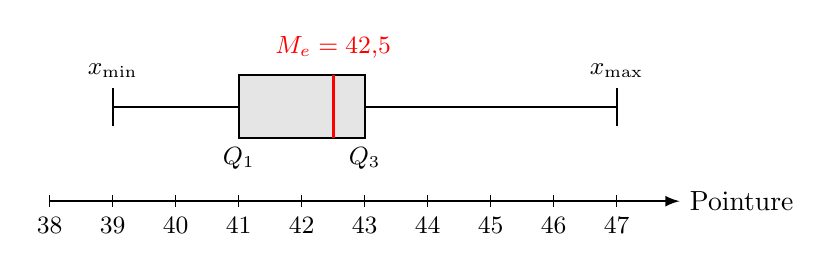
\begin{tikzpicture}[scale=0.8]
			\draw[->, >=latex, thick] (38,0) -- (48,0) node[right] {Pointure};
			\foreach \x in {38,39,...,47} { \draw (\x,0.1) -- (\x,-0.1) node[below] {\small \x}; }
			\draw[thick, fill=gray!20] (41,1) rectangle (43,2);
			\draw[very thick, red] (42.5,1) -- (42.5,2) node[above=2pt, red] {\small $M_e = 42{,}5$};
			\draw[thick] (39,1.5) -- (41,1.5);
			\draw[thick] (43,1.5) -- (47,1.5);
			\draw[thick] (39,1.2) -- (39,1.8) node[above] {\small $x_{\min}$};
			\draw[thick] (47,1.2) -- (47,1.8) node[above] {\small $x_{\max}$};
			\node[below] at (41,1) {\small $Q_1$};
			\node[below] at (43,1) {\small $Q_3$};
		\end{tikzpicture}
	\end{center}

	\textbf{Interprétation :}
	\begin{itemize}
		\item La boîte centrale contient $50\,\%$ des effectifs : au moins la moitié des joueurs chaussent une pointure comprise entre $41$ ($Q_1$) et $43$ ($Q_3$).
		\item Au moins $50\,\%$ des joueurs ont une pointure inférieure ou égale à $42{,}5$ ($M_e$).
	\end{itemize}
\end{ex}

\newpage

\subsection{Variance et écart-type}

\begin{defin}[Variance et écart-type]
	Soit une série statistique de moyenne $\bar{x}$, dont les valeurs $x_i$ ont pour effectifs $n_i$ (avec un effectif total $N$).
	\begin{itemize}
		\item La \textbf{variance}, notée $V$, est la moyenne des carrés des écarts à la moyenne :
		      \[
			      V = \dfrac{n_1\pa{x_1 - \bar{x}}^2 + n_2\pa{x_2 - \bar{x}}^2 + \dots + n_k\pa{x_k - \bar{x}}^2}{N}
		      \]
		\item L'\textbf{écart-type}, noté $\sigma$, est la racine carrée de la variance :
		      \[
			      \sigma = \sqrt{V}
		      \]
	\end{itemize}
\end{defin}

\begin{remarque}
	L'écart-type s'exprime dans la même unité que les données de la série, contrairement à la variance.

	Il mesure la dispersion des valeurs autour de la moyenne arithmétique : plus $\sigma$ est petit, plus la série est \textbf{concentrée} autour de sa \textbf{moyenne}.
\end{remarque}

\begin{methode}[Calculer la variance et l'écart-type]
	On considère la distribution suivante :
	\begin{center}
		\rnc{\arraystretch}{1.2}
		\begin{tabular}{|c|c|c|c|c|} \hline
			\cellcolor{gray!30} $x_i$ & 1 & 2 & 3 & 4 \\ \hline
			\cellcolor{gray!30} $n_i$ & 5 & 9 & 3 & 1 \\ \hline
		\end{tabular}
	\end{center}

	\begin{correction}
		\nline
		\begin{enumerate}
			\item \textbf{Calcul de la moyenne $\bar{x}$ :}

			      \[
				      N = 5 + 9 + 3 + 1 = 18 \quad \text{et} \quad \bar{x} = \dfrac{5 \times 1 + 9 \times 2 + 3 \times 3 + 1 \times 4}{18} = \dfrac{36}{18} = 2
			      \]

			\item \textbf{Calcul de la variance $V$ via le tableau d'écarts :}
			      \ms
			      \begin{center}
				      \rnc{\arraystretch}{1.2}
				      \begin{tabular}{|c|c|c|c|c|} \hline
					      \cellcolor{gray!30} Valeur $x_i$           & 1                & 2                & 3                & 4                \\ \hline
					      \cellcolor{gray!30} Effectif $n_i$         & 5                & 9                & 3                & 1                \\ \hline
					      \cellcolor{gray!30} $x_i - \bar{x}$        & $-1$             & $0$              & $1$              & $2$              \\ \hline
					      \cellcolor{gray!30} $(x_i - \bar{x})^2$    & $1$              & $0$              & $1$              & $4$              \\ \hline
					      \cellcolor{gray!30} $n_i(x_i - \bar{x})^2$ & $5 \times 1 = 5$ & $9 \times 0 = 0$ & $3 \times 1 = 3$ & $1 \times 4 = 4$ \\ \hline
				      \end{tabular}
			      \end{center}

			      \ms

			      On effectue le calcul de la variance grâce à la dernière ligne :
			      \[
				      V = \dfrac{5 + 0 + 3 + 4}{18} = \dfrac{12}{18} = \dfrac{2}{3} \approx 0{,}67
			      \]

			\item \textbf{Calcul de l'écart-type $\sigma$ :}
			      \[
				      \sigma = \sqrt{\dfrac{2}{3}} \approx 0{,}82
			      \]
		\end{enumerate}
	\end{correction}
\end{methode}

\newpage

\section{Représentations graphiques}

Le choix de la représentation graphique dépend de la nature du caractère étudié (discret ou continu) et de ce que l'on cherche à mettre en évidence.

\subsection{Caractère discret : Diagramme en bâtons et diagramme circulaire}

\begin{defin}[Diagramme en bâtons]
	Pour une série statistique à \textbf{caractère discret}, on représente chaque valeur par un bâton vertical dont la hauteur est proportionnelle à l'effectif (ou à la fréquence).
\end{defin}

\begin{ex}[Diagramme en bâtons]
	On reprend le nombre de frères et sœurs des $21$ élèves de Première STMG :

	\begin{center}
		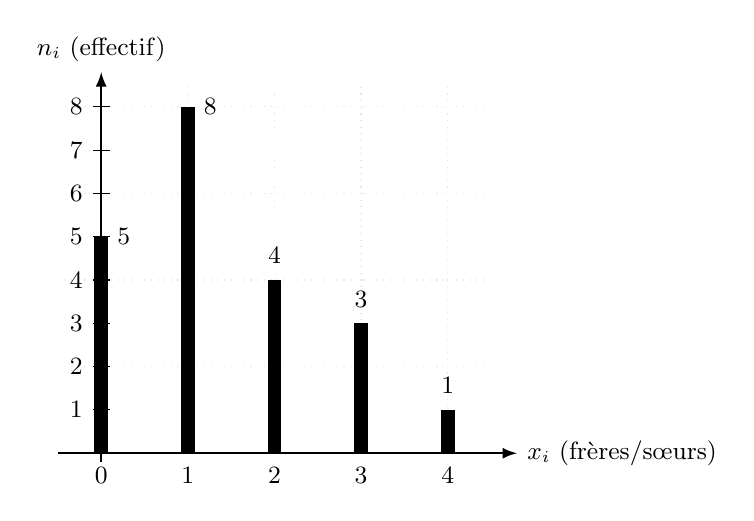
\begin{tikzpicture}[scale=1.1, baseline=(current bounding box.center), y=5mm]
			\draw[gray!20, dotted] (-0.5,0) grid (4.5,8.5);
			\draw[->, >=latex, thick] (-0.5,0) -- (4.8,0) node[right] {\small $x_i$ (frères/sœurs)};
			\draw[->, >=latex, thick] (0,-0.2) -- (0,8.8) node[above] {\small $n_i$ (effectif)};
			\foreach \y in {1,2,...,8} { \draw (0.1,\y) -- (-0.1,\y) node[left] {\small \y}; }
			\draw[line width=5pt] (0,0) -- (0,5) node[above,right] {\small 5};
			\draw[line width=5pt] (1,0) -- (1,8) node[above,right] {\small 8};
			\draw[line width=5pt] (2,0) -- (2,4) node[above] {\small 4};
			\draw[line width=5pt] (3,0) -- (3,3) node[above] {\small 3};
			\draw[line width=5pt] (4,0) -- (4,1) node[above] {\small 1};
			\foreach \x in {0,1,2,3,4} { \node[below] at (\x,-0.1) {\small \x}; }
		\end{tikzpicture}
	\end{center}
\end{ex}

\begin{defin}[Diagramme circulaire (ou « camembert »)]
	Un \textbf{diagramme circulaire} partage un disque en secteurs dont la mesure de l'angle (en degrés) est proportionnelle à l'effectif ou à la fréquence de chaque modalité :
	\[
		\text{Angle (en degrees)} = \text{Fréquence} \times 360^\circ = \dfrac{n_i}{N} \times 360^\circ
	\]
\end{defin}

\begin{ex}[Diagramme circulaire]
	Pour une répartition de $24$ élèves selon leur filière de spécialité :
	\begin{itemize}
		\item Mercatique : $12$ élèves ($50\,\% \rightarrow 180^\circ$)
		\item Gestion-Finance : $8$ élèves ($\approx 33{,}3\,\% \rightarrow 120^\circ$)
		\item R.H. : $4$ élèves ($\approx 16{,}7\,\% \rightarrow 60^\circ$)
	\end{itemize}

	\begin{center}
		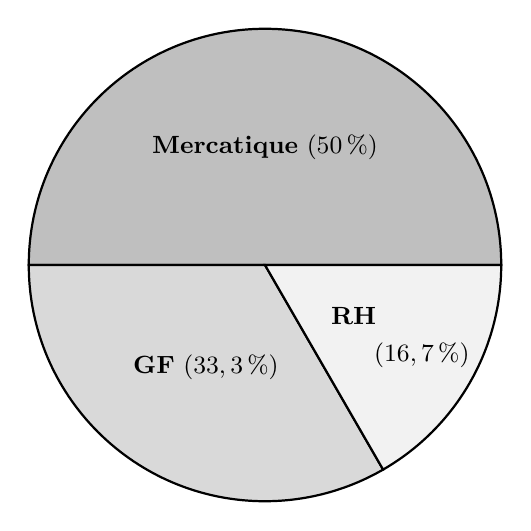
\begin{tikzpicture}[baseline=(current bounding box.center)]
			\fill[gray!50] (0,0) -- (0:3) arc (0:180:3) -- cycle;
			\draw[thick] (0,0) -- (0:3) arc (0:180:3) -- cycle;
			\node at (90:1.5) {\small \textbf{Mercatique} ($50\,\%$)};
			\fill[gray!30] (0,0) -- (180:3) arc (180:300:3) -- cycle;
			\draw[thick] (0,0) -- (180:3) arc (180:300:3) -- cycle;
			\node at (240:1.5) {\small \textbf{GF} ($33,3\,\%$)};
			\fill[gray!10] (0,0) -- (300:3) arc (300:360:3) -- cycle;
			\draw[thick] (0,0) -- (300:3) arc (300:360:3) -- cycle;
			\node at (330:1.3) {\small \textbf{RH}};
			\node at (330:2.3) {\small ($16,7\,\%$)};
		\end{tikzpicture}
	\end{center}
\end{ex}

\newpage

\subsection{Caractère continu : Histogramme et Polygon des E.C.C.}

\begin{defin}[Histogramme]
	Pour une série regroupée en classes, l'\textbf{histogramme} est constitué de rectangles adjacents dont l'\textbf{aire} est proportionnelle à l'effectif de la classe.
\end{defin}

\begin{remarque}
	Si toutes les classes ont la même amplitude, la \textbf{hauteur} de chaque rectangle est alors directement proportionnelle à l'effectif.
\end{remarque}

\begin{ex}[Histogramme à classes d'amplitudes égales]
	On reprend la taille des $24$ élèves de STMG regroupés par classes de $5\text{ cm}$ :
	\begin{center}
		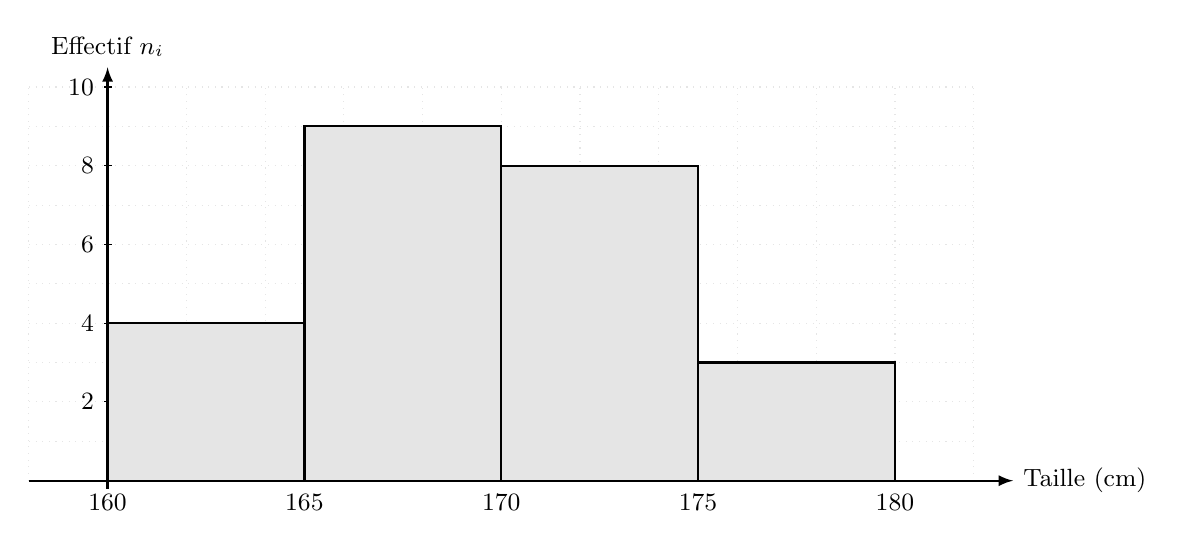
\begin{tikzpicture}[scale=0.5, baseline=(current bounding box.center)]
			\draw[gray!20, dotted] (158,0) grid[xstep=2, ystep=1] (182,10);
			\draw[->, >=latex, thick] (158,0) -- (183,0) node[right] {\small Taille (cm)};
			\draw[->, >=latex, thick] (160,-0.2) -- (160,10.5) node[above] {\small Effectif $n_i$};
			\foreach \y in {2,4,6,8,10} { \draw (160.1,\y) -- (159.9,\y) node[left] {\small \y}; }
			\draw[fill=gray!20, thick] (160,0) rectangle (165,4);
			\draw[fill=gray!20, thick] (165,0) rectangle (170,9);
			\draw[fill=gray!20, thick] (170,0) rectangle (175,8);
			\draw[fill=gray!20, thick] (175,0) rectangle (180,3);
			\foreach \x in {160,165,170,175,180} { \node[below] at (\x,-0.1) {\small \x}; }
		\end{tikzpicture}
	\end{center}
\end{ex}

\subsection{Polygone des effectifs cumulés croissants (E.C.C.)}

\begin{defin}[Polygone des E.C.C.]
	Le \textbf{polygone des effectifs cumulés croissants} (ou des fréquences cumulées croissantes) permet de visualiser la répartition cumulée des données d'un caractère continu.
	\begin{itemize}
		\item On place les points dont l'\textbf{abscisse} est la borne supérieure de la classe et l'\textbf{ordonnée} est l'E.C.C. (ou la F.C.C.) correspondant.
		\item On relie ces points par des segments de droite, en partant du point correspondant à la borne inférieure de la première classe d'ordonnée $0$.
	\end{itemize}
\end{defin}

\begin{ex}[Tracé du polygone des E.C.C. et détermination graphique de la médiane]
	On reprend le tableau des tailles des $24$ élèves de STMG :

	\begin{center}
		\rnc{\arraystretch}{1.3}
		\begin{tabular}{|>{\columncolor{gray!30}}c|c|c|c|c|} \hline
			Classes $[a ; b[$ & $[160 ; 165[$ & $[165 ; 170[$ & $[170 ; 175[$ & $[175 ; 180[$ \\ \hline
			Effectifs $n_i$   & 4             & 9             & 8             & 3             \\ \hline
			E.C.C.            & 4             & 13            & 21            & 24            \\ \hline
		\end{tabular}
	\end{center}

	Les points à placer sont : $(160 ; 0)$, $(165 ; 4)$, $(170 ; 13)$, $(175 ; 21)$ et $(180 ; 24)$.

	\begin{center}
		\begin{tikzpicture}[scale=0.4, baseline=(current bounding box.center)]
			\draw[gray!90, dotted] (158,0) grid[xstep=2, ystep=2] (182,26);
			\draw[->, >=latex, thick] (158,0) -- (183,0) node[right] {Taille (cm)};
			\draw[->, >=latex, thick] (158,-0.2) -- (158,26.5) node[above] {E.C.C.};
			\foreach \y in {0,4,8,12,16,20,24} { \draw (158.3,\y) -- (157.7,\y) node[left] {\y}; }
			\draw[line width=0.5mm, gray, mark=*] plot coordinates { (160,0) (165,4) (170,13) (175,21) (180,24) };
			\draw[dashed, thick, ->] (158,12) -- (169.44,12);
			\draw[dashed, thick, ->] (169.44,12) -- (169.44,0);
			\node[left, xshift=-12mm] at (160,12) {$\dfrac{N}{2}\rarr$};
			\node[below, yshift=-6mm] at (169.44,0) {$M_e \approx 169,4$};
			\foreach \x in {160,165,170,175,180} { \draw (\x,-0.2) -- (\x,0.2); \node[below] at (\x,-0.1) {\x}; }
		\end{tikzpicture}
	\end{center}

	\begin{rem}
		Sur le polygone des E.C.C., l'abscisse correspondant à l'ordonnée $\dfrac{N}{2} = 12$ donne une estimation graphique de la \textbf{médiane} $M_e \approx 169{,}4\text{ cm}$.
	\end{rem}
\end{ex}

% \chapter{Probabilités}

\section{Vocabulaire des expériences aléatoires}

\begin{defin}[Expérience aléatoire]
	Une expérience est dite \textbf{aléatoire} lorsqu'elle peut conduire à plusieurs résultats différents et que l'on ne peut pas prévoir à l'avance lequel de ces résultats va se produire.
\end{defin}

\begin{ex}
	\nline
	\begin{wrapstuff}[r]
		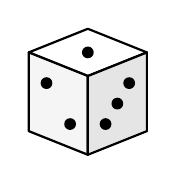
\begin{tikzpicture}[scale=0.5]
			% Style des points du dé (plus gros)
			\tikzset{ pion/.style={circle, fill=black, inner sep=1.5pt} }
			\draw[thick, fill=white, join=round]
			(0,2) -- (1.5,2.6) -- (0,3.2) -- (-1.5,2.6) -- cycle;
			\begin{scope}[cm={0.75, 0.3, -0.75, 0.3, (0, 2.6)}]
				\node[pion] at (0,0) {};
			\end{scope}
			\draw[thick, fill=gray!8, join=round]
			(0,0) -- (0,2) -- (-1.5,2.6) -- (-1.5,0.6) -- cycle;
			\begin{scope}[cm={-0.75, 0.3, 0, 1, (-0.75, 1.3)}]
				\node[pion] at (-0.4, -0.4) {};
				\node[pion] at (0.4, 0.4) {};
			\end{scope}
			\draw[thick, fill=gray!20, join=round] (0,0) -- (0,2) -- (1.5,2.6) -- (1.5,0.6) -- cycle;
			\begin{scope}[cm={0.75, 0.3, 0, 1, (0.75, 1.3)}]
				\node[pion] at (-0.4, -0.4) {};
				\node[pion] at (0, 0) {};
				\node[pion] at (0.4, 0.4) {};
			\end{scope}
		\end{tikzpicture}
	\end{wrapstuff}

	On lance le dé représenté ci-contre et on regarde le numéro inscrit sur la face du dessus.

	On ne peut pas prévoir, avant de lancer, quel numéro va sortir~: c'est une expérience aléatoire.

	\phantom{x}

	\phantom{x}
\end{ex}

\begin{defin}[Univers]
	L'ensemble de \textbf{tous} les résultats possibles d'une expérience aléatoire s'appelle l'\textbf{univers} de l'expérience.

	On le note en général $\Omega$ (la lettre grecque \og oméga \fg{}).

	Chaque résultat possible s'appelle une \textbf{issue}.
\end{defin}

\begin{ex}
	\nline
	\begin{itemize}
		\item Expérience aléatoire~: \og On lance un dé à six faces et on note le numéro obtenu \fg{}
		\item Univers~: $\Omega = \left\{ \epsdice{1};\epsdice{2};\epsdice{3};\epsdice{4};\epsdice{5};\epsdice{6} \right\}$
		\item Chacun des six résultats possibles est une \textbf{issue} de l'expérience.
	\end{itemize}
\end{ex}

\begin{defin}[Événement]
	Un \textbf{événement} est un ensemble d'issues d'une expérience aléatoire, c'est-à-dire une \textbf{partie} de l'univers $\Omega$.

	Lorsqu'un événement n'est constitué que d'une seule issue, on dit que c'est un \textbf{événement élémentaire}.
\end{defin}

\begin{ex}
	On reprend l'expérience \og lancer un dé \fg{} et $\Omega = \left\{ \epsdice{1};\epsdice{2};\epsdice{3};\epsdice{4};\epsdice{5};\epsdice{6} \right\}$.
	\begin{itemize}
		\item $A~:$ \og Obtenir un nombre pair \fg{} $\quad\Rarr\quad A = \left\{ \epsdice{2};\epsdice{4};\epsdice{6} \right\}$
		\item $B~:$ \og Obtenir un nombre supérieur ou égal à 5 \fg{} $\quad\Rarr\quad B = \left\{ \epsdice{5};\epsdice{6} \right\}$
		\item $C~:$ \og Obtenir le numéro 3 \fg{} $\quad\Rarr\quad C = \left\{ \epsdice{3} \right\}$ est un événement \textbf{élémentaire}.
	\end{itemize}
\end{ex}

\begin{rem}
	\nline
	\begin{itemize}
		\item L'événement \textbf{certain} est l'univers $\Omega$ tout entier~: il est toujours réalisé, quelle que soit l'issue obtenue.
		\item L'événement \textbf{impossible} est l'ensemble vide, noté $\varnothing$~: aucune issue ne peut le réaliser.
	\end{itemize}
\end{rem}

\begin{ex}
	Avec l'expérience aléatoire précédente~:
	\begin{itemize}
		\item \og Obtenir un nombre compris entre 1 et 6 \fg{} est l'événement \textbf{certain}.
		\item \og Obtenir le nombre 9 \fg{} est un événement \textbf{impossible}.
	\end{itemize}
\end{ex}

\begin{ex}
	\nline
	\begin{itemize}
		\item \textbf{Expérience aléatoire~:} \og On choisit un élève au hasard dans la classe et on compte son nombre de frères et s\oe{}urs \fg{} (dans une classe où personne n'en a plus de 4).
		\item \textbf{Univers~:} $\Omega = \left\{ 0 ; 1 ; 2 ; 3 ; 4 \right\}$
		\item Chaque nombre de $0$ à $4$ est une \textbf{issue} de l'expérience.
		\item \textbf{Événements~:}
		      \begin{itemize}
			      \item $A~:$ \og L'élève a au moins deux frères et s\oe{}urs \fg{} $\quad\Rarr\quad A = \left\{ 2 ; 3 ; 4 \right\}$
			      \item $B~:$ \og L'élève a un nombre pair de frères et s\oe{}urs \fg{} $\quad\Rarr\quad B = \left\{ 0 ; 2 ; 4 \right\}$
			      \item $C~:$ \og L'élève est enfant unique \fg{} $\quad\Rarr\quad C = \left\{ 0 \right\}$ est un événement \textbf{élémentaire}.
			      \item \og L'élève a moins de 5 frères et s\oe{}urs \fg{} est l'événement \textbf{certain}.
			      \item \og L'élève a 10 frères et s\oe{}urs \fg{} est un événement \textbf{impossible}.
		      \end{itemize}
	\end{itemize}
\end{ex}

\begin{ex}
	\nline
	\begin{itemize}
		\item \textbf{Expérience aléatoire~:} \og On consulte l'application météo pour relever le temps qu'il fera samedi après-midi \fg{}
		\item \textbf{Univers~:} $\Omega = \left\{ \text{Soleil} ; \text{Nuageux} ; \text{Pluie} ; \text{Neige} \right\}$
		\item Chaque type de temps est une \textbf{issue} de l'expérience.
		\item \textbf{Événements~:}
		      \begin{itemize}
			      \item $A~:$ \og Il y a des précipitations \fg{} $\quad\Rarr\quad A = \left\{ \text{Pluie} ; \text{Neige} \right\}$
			      \item $B~:$ \og Il ne pleut pas \fg{} $\quad\Rarr\quad B = \left\{ \text{Soleil} ; \text{Nuageux} ; \text{Neige} \right\}$
			      \item $C~:$ \og Il fait soleil \fg{} $\quad\Rarr\quad C = \left\{ \text{Soleil} \right\}$ est un événement \textbf{élémentaire}.
			      \item \og Le temps correspond à l'une des quatre conditions météo \fg{} est l'événement \textbf{certain}.
			      \item \og Il tombe des grenouilles \fg{} est un événement \textbf{impossible}.
		      \end{itemize}
	\end{itemize}
\end{ex}

\section{Calculer des probabilités}

\subsection{Loi de probabilité}

\begin{defin}[Loi de probabilité]
	Soit $\Omega = \left\{ e_1 ; e_2 ; \ldots ; e_n \right\}$ l'univers associé à une expérience aléatoire.

	\textbf{Définir une loi de probabilité} sur $\Omega$, c'est associer à chaque issue $e_i$ un nombre réel $p_i$, appelé \textbf{probabilité} de l'issue $e_i$ et noté $P(e_i)$, tel que~:

	\begin{itemize}
		\item Chaque probabilité est comprise entre $0$ et $1$~: $\quad 0 \le P(e_i) \le 1$
		\item La somme de toutes les probabilités vaut $1$~: $\quad P(e_1) + P(e_2) + \ldots + P(e_n) = 1$
	\end{itemize}

	On présente souvent une loi de probabilité sous forme d'un tableau.
\end{defin}

\begin{ex}
	\nline
	\begin{wrapstuff}[r]
		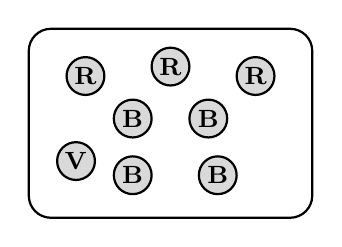
\begin{tikzpicture}[scale=0.6]
			\draw[thick, rounded corners=8pt] (-3,-2) rectangle (3,2);
			\foreach \p/\l in { (-1.8, 1.0)/R, (0.0, 1.2)/R, (1.8, 1.0)/R, (-2.0,-0.8)/V, (-0.8, 0.1)/B, (0.8, 0.1)/B, (-0.8,-1.1)/B, (1.0,-1.1)/B } { \filldraw[fill=black!15, draw=black, thick] \p circle (0.4); \node at \p {\small\textbf{\l}}; }
		\end{tikzpicture}
	\end{wrapstuff}
	Un sac opaque contient $8$ jetons indiscernables au toucher~:

	\begin{itemize}
		\item $3$ jetons rouges
		\item $1$ jeton vert
		\item $4$ jetons bleus.
	\end{itemize}

	On tire un jeton au hasard et on note sa couleur.

	La situation n'est pas équiprobable~: il y a plus de jetons bleus que de jetons verts.

	On obtient la loi de probabilité suivante~:
	\[
		\begin{array}{|c|c|c|c|} \hline
			\cellcolor{gray!30} e_i                          & \text{Rouge}           & \text{Vert}            & \text{Bleu}          \\ \hline
			\cellcolor{gray!30} \rule[-4mm]{0mm}{11mm}P(e_i) & \dfrac{3}{8} = 0{,}375 & \dfrac{1}{8} = 0{,}125 & \dfrac{4}{8} = 0{,}5 \\ \hline
		\end{array}
	\]

	On vérifie bien que~: $\quad 0{,}375 + 0{,}125 + 0{,}5 = 1$
\end{ex}

\begin{defin}[Probabilité d'un événement]
	La \textbf{probabilité} d'un événement $A$, notée $P(A)$, est la \textbf{somme} des probabilités des issues qui le composent.
\end{defin}

\begin{ex}
	\nline
	\begin{itemize}
		\item \textbf{Expérience aléatoire~:} \og On choisit une personne au hasard en France et on note son groupe sanguin (système ABO) \fg{}

		\item La loi de probabilité associée est la suivante~:

		      \begin{center}
			      \begin{tabular}{|c|c|c|c|c|} \hline
				      \cellcolor{gray!30}Groupe sanguin $e_i$ & $A$      & $O$      & $B$      & $AB$     \\ \hline
				      \cellcolor{gray!30}$P(e_i)$             & $0{,}44$ & $0{,}42$ & $0{,}10$ & $0{,}04$ \\ \hline
			      \end{tabular}
		      \end{center}
		      \ms
		\item Soit $R~:$ \og La personne possède un groupe sanguin rare (B ou AB) \fg{}, donc $R = \left\{ B ; AB \right\}$.
		      \[
			      P(R) = P(B) + P(AB) = 0{,}10 + 0{,}04 = 0{,}14
		      \]
	\end{itemize}
\end{ex}

\begin{ex}[Étude d'un jeu de dominos]
	\nline
	\begin{wrapstuff}[r]
		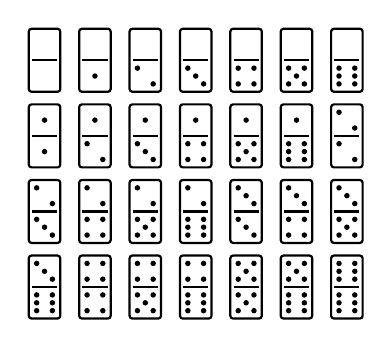
\begin{tikzpicture}[scale=0.4]
			\tikzset{ dot/.style={circle, fill=black, inner sep=0.7pt} }
			\newcommand{\drawdots}[3]{
				\ifnum#3=1
					\node[dot] at (#1,#2) {};
				\fi
				\ifnum#3=2
					\node[dot] at (#1-0.25,#2+0.25) {};
					\node[dot] at (#1+0.25,#2-0.25) {};
				\fi
				\ifnum#3=3
					\node[dot] at (#1-0.25,#2+0.25) {};
					\node[dot] at (#1,#2) {};
					\node[dot] at (#1+0.25,#2-0.25) {};
				\fi
				\ifnum#3=4
					\node[dot] at (#1-0.25,#2+0.25) {};
					\node[dot] at (#1+0.25,#2+0.25) {};
					\node[dot] at (#1-0.25,#2-0.25) {};
					\node[dot] at (#1+0.25,#2-0.25) {};
				\fi
				\ifnum#3=5
					\node[dot] at (#1-0.25,#2+0.25) {};
					\node[dot] at (#1+0.25,#2+0.25) {};
					\node[dot] at (#1,#2) {};
					\node[dot] at (#1-0.25,#2-0.25) {};
					\node[dot] at (#1+0.25,#2-0.25) {};
				\fi
				\ifnum#3=6
					\node[dot] at (#1-0.25,#2+0.25) {};
					\node[dot] at (#1+0.25,#2+0.25) {};
					\node[dot] at (#1-0.25,#2) {};
					\node[dot] at (#1+0.25,#2) {};
					\node[dot] at (#1-0.25,#2-0.25) {};
					\node[dot] at (#1+0.25,#2-0.25) {};
				\fi
			}
			\foreach \valH/\valB [count=\col from 0] in {0/0, 0/1, 0/2, 0/3, 0/4, 0/5, 0/6} {
					\pgfmathsetmacro{\x}{\col * 1.6}
					\pgfmathsetmacro{\y}{0}
					\draw[thick, rounded corners=1pt, fill=white] (\x-0.5, \y-1) rectangle (\x+0.5, \y+1);
					\draw[thick] (\x-0.4, \y) -- (\x+0.4, \y);
					\drawdots{\x}{\y+0.5}{\valH}
					\drawdots{\x}{\y-0.5}{\valB}
				}
			\foreach \valH/\valB [count=\col from 0] in {1/1, 1/2, 1/3, 1/4, 1/5, 1/6, 2/2} {
					\pgfmathsetmacro{\x}{\col * 1.6}
					\pgfmathsetmacro{\y}{-2.4}
					\draw[thick, rounded corners=1pt, fill=white] (\x-0.5, \y-1) rectangle (\x+0.5, \y+1);
					\draw[thick] (\x-0.4, \y) -- (\x+0.4, \y);
					\drawdots{\x}{\y+0.5}{\valH}
					\drawdots{\x}{\y-0.5}{\valB}
				}
			\foreach \valH/\valB [count=\col from 0] in {2/3, 2/4, 2/5, 2/6, 3/3, 3/4, 3/5} {
					\pgfmathsetmacro{\x}{\col * 1.6}
					\pgfmathsetmacro{\y}{-4.8}
					\draw[thick, rounded corners=1pt, fill=white] (\x-0.5, \y-1) rectangle (\x+0.5, \y+1);
					\draw[thick] (\x-0.4, \y) -- (\x+0.4, \y);
					\drawdots{\x}{\y+0.5}{\valH}
					\drawdots{\x}{\y-0.5}{\valB}
				}
			\foreach \valH/\valB [count=\col from 0] in {3/6, 4/4, 4/5, 4/6, 5/5, 5/6, 6/6} {
					\pgfmathsetmacro{\x}{\col * 1.6}
					\pgfmathsetmacro{\y}{-7.2}
					\draw[thick, rounded corners=1pt, fill=white] (\x-0.5, \y-1) rectangle (\x+0.5, \y+1);
					\draw[thick] (\x-0.4, \y) -- (\x+0.4, \y);
					\drawdots{\x}{\y+0.5}{\valH}
					\drawdots{\x}{\y-0.5}{\valB}
				}
		\end{tikzpicture}
	\end{wrapstuff}

	Un jeu de dominos traditionnel contient $28$ pièces distinctes marquant chacune deux nombres de points de $0$ à $6$ (du double zéro au double six).

	\begin{itemize}
		\item \textbf{Expérience aléatoire~:} \og On tire au hasard un domino dans le jeu et on calcule la somme des points inscrits sur la pièce \fg{}

		\item \textbf{Univers~:} La somme minimale possible est $0+0=0$ et la somme maximale est $6+6=12$.
		      \[ \Omega = \left\{ 0 ; 1 ; 2 ; 3 ; 4 ; 5 ; 6 ; 7 ; 8 ; 9 ; 10 ; 11 ; 12 \right\} \]
		      L'univers contient $13$ issues.

		\item \textbf{Établissement de la loi de probabilité de la somme~:}

		      Chaque domino a la même chance d'être tiré $\pa{\frac{1}{28}}$, mais certaines sommes peuvent être obtenues avec plusieurs dominos différents~:

		      \small

		      \begin{multicols}{2}
			      \begin{itemize}[itemsep=1mm]
				      \item Somme = $0$~: $\{0-0\}$  $\ \Rarr\  P(0) = \frac{1}{28}$
				      \item Somme = $1$~: $\{0-1\}$  $\ \Rarr\  P(1) = \frac{1}{28}$
				      \item Somme = $2$~: $\{0-2\,;\,1-1\}$  $\ \Rarr\  P(2) = \frac{2}{28}$
				      \item Somme = $3$~: $\{0-3\,;\,1-2\}$  $\ \Rarr\  P(3) = \frac{2}{28}$
				      \item Somme = $4$~: $\{0-4\,;\,1-3\,;\,2-2\}$  $\ \Rarr\  P(4) = \frac{3}{28}$
				      \item Somme = $5$~: $\{0-5\,;\,1-4\,;\,2-3\}$  $\ \Rarr\  P(5) = \frac{3}{28}$
				      \item Somme = $6$~: $\{0-6\,;\,1-5\,;\,2-4\,;\,3-3\}$  $\ \Rarr\  P(6) = \frac{4}{28}$
				      \item Somme = $7$~: $\{1-6\,;\,2-5\,;\,3-4\}$  $\ \Rarr\  P(7) = \frac{3}{28}$
				      \item Somme = $8$~: $\{2-6\,;\,3-5\,;\,4-4\}$  $\ \Rarr\  P(8) = \frac{3}{28}$
				      \item Somme = $9$~: $\{3-6\,;\,4-5\}$  $\ \Rarr\  P(9) = \frac{2}{28}$
				      \item Somme = $10$~: $\{4-6\,;\,5-5\}$  $\ \Rarr\  P(10) = \frac{2}{28}$
				      \item Somme = $11$~: $\{5-6\}$  $\ \Rarr\  P(11) = \frac{1}{28}$
				      \item Somme = $12$~: $\{6-6\}$  $\ \Rarr\  P(12) = \frac{1}{28}$
			      \end{itemize}
		      \end{multicols}
		      \normalsize

		      On résume la loi de probabilité dans le tableau suivant~:

		      \begin{center}
			      \rnc{\arraystretch}{1.3}
			      \begin{tabular}{|c|c|c|c|c|c|c|c|c|c|c|c|c|c|}
				      \hline
				      \cellcolor{gray!30}  $e_i$                         & $0$             & $1$             & $2$             & $3$             & $4$             & $5$             & $6$             & $7$             & $8$             & $9$             & $10$            & $11$            & $12$            \\ \hline
				      \cellcolor{gray!30} \rule[-4mm]{0mm}{10mm}$P(e_i)$ & $\dfrac{1}{28}$ & $\dfrac{1}{28}$ & $\dfrac{2}{28}$ & $\dfrac{2}{28}$ & $\dfrac{3}{28}$ & $\dfrac{3}{28}$ & $\dfrac{4}{28}$ & $\dfrac{3}{28}$ & $\dfrac{3}{28}$ & $\dfrac{2}{28}$ & $\dfrac{2}{28}$ & $\dfrac{1}{28}$ & $\dfrac{1}{28}$ \\ \hline
			      \end{tabular}
		      \end{center}

		      \ms

		\item \textbf{Calcul de la probabilité d'un événement~:}

		      Soit $S~:$ \og Obtenir un domino dont la somme des points est strictement supérieure à $7$ \fg{}.

		      Les issues composant l'événement $S$ sont $S = \left\{ 8 ; 9 ; 10 ; 11 ; 12 \right\}$.

		      Par définition, $P(S)$ est la \textbf{somme des probabilités des issues} qui le composent~:
		      \[
			      \def\arraystretch{1.5}
			      \begin{array}{rccccccccccl}
				      P(S) & = & P(8)          & + & P(9)          & + & P(10)         & + & P(11)         & + & P(12)         &                 \\
				           & = & \dfrac{3}{28} & + & \dfrac{2}{28} & + & \dfrac{2}{28} & + & \dfrac{1}{28} & + & \dfrac{1}{28} & = \dfrac{9}{28}
			      \end{array}
		      \]
		      La probabilité de tirer un domino dont la somme des points est supérieure à $7$ est donc égale à $\dfrac{9}{28}$.
	\end{itemize}
\end{ex}
\subsection{Événement contraire}

\begin{defin}[Événement contraire]
	Soit $A$ un événement d'un univers $\Omega$.

	L'\textbf{événement contraire} de $A$, noté $\bar{A}$ (et lu \og $A$ barre \fg{}), est l'événement constitué de toutes les issues de $\Omega$ qui \textbf{n'appartiennent pas} à $A$.
\end{defin}

\begin{prop}[Probabilité de l'événement contraire]
	Pour tout événement $A$, la somme des probabilités de $A$ et de son contraire est égale à $1$~:
	\[ P\pa{A} + P\pa{\bar{A}} = 1 \quad\Rarr\quad P\pa{\bar{A}} = 1 - P(A) \]
\end{prop}

\begin{ex}[Calcul à l'aide de l'événement contraire]
	On reprend le jeu de $28$ dominos de l'exemple précédent. On tire un domino au hasard.

	Soit $E$ l'événement~: \og Obtenir un domino dont la somme des points est au moins égale à $2$ \fg{}.

	\begin{itemize}
		\item Calculer directement $P(E)$ nécessiterait d'additionner les probabilités des issues $2, 3, 4, 5, 6, 7, 8, 9, 10, 11$ et $12$ ($11$ calculs).

		\item L'événement contraire de $E$ est $\bar{E}~:$ \og Obtenir une somme strictement inférieure à $2$ \fg{}.

		      Les seules issues réalisant $\bar{E}$ sont $0$ et $1$, soit $\bar{E} = \left\{ 0 ; 1 \right\}$.

		\item On calcule facilement la probabilité de $\bar{E}$~:
		      \[ P\pa{\bar{E}} = P(0) + P(1) = \dfrac{1}{28} + \dfrac{1}{28} = \dfrac{2}{28} \]

		\item On en déduit alors la probabilité de $E$~:
		      \[ P(E) = 1 - P\pa{\bar{E}} = 1 - \dfrac{2}{28} = \dfrac{26}{28} = \dfrac{13}{14} \]
	\end{itemize}
\end{ex}

\subsection{Situations d'équiprobabilité}

\begin{defin}[Équiprobabilité]
	On dit qu'il y a \textbf{équiprobabilité} lorsque toutes les issues de l'univers ont la \textbf{même} probabilité de se réaliser.

	On dit aussi que la loi de probabilité est \textbf{équirépartie}.
\end{defin}

\begin{prop}
	Dans une situation d'équiprobabilité sur un univers $\Omega$ constitué de $n$ issues, la probabilité d'un événement $A$ est~:
	\[
		P(A) = \dfrac{\text{nombre d'issues favorables à } A}{\text{nombre d'issues total}} = \dfrac{\text{Card}(A)}{\text{Card}(\Omega)}
	\]

	\ldots où $\text{Card}(A)$ désigne le \textbf{cardinal} de l'ensemble $A$, c'est-à-dire son nombre d'éléments (d'issues).
\end{prop}

\begin{ex}
	On tire au hasard une carte dans un jeu de $32$ cartes bien mélangé.
	\begin{itemize}
		\item L'univers est $\Omega = \left\{ \text{7 de C\oe{}ur} ; \text{8 de C\oe{}ur} ; \ldots ; \text{As de Pique} \right\}$ et contient $32$ issues.
		\item Toutes les cartes ont la même chance d'être tirées~: il y a \textbf{équiprobabilité}.
		\item La probabilité de tirer une carte précise (par exemple l'As de C\oe{}ur) est $P(\text{\og As de C\oe{}ur \fg{}}) = \dfrac{1}{32}$.
	\end{itemize}
\end{ex}

\begin{ex}
	On lance un dé \textbf{non truqué} à six faces. Toutes les faces ont la même chance de sortir~: la situation est équiprobable, et $P\pa{\epsdice{1}} = P\pa{\epsdice{2}} = \ldots = P\pa{\epsdice{6}} = \dfrac{1}{6}$.

	Soit $A~:$ \og Obtenir un multiple de 3 \fg{}, donc $A = \left\{ \epsdice{3};\epsdice{6} \right\}$.
	\[
		P(A) = \dfrac{\text{Card}(A)}{\text{Card}(\Omega)} = \dfrac{2}{6} = \dfrac{1}{3}
	\]
\end{ex}

\section{Intersection et union d'événements}

\begin{defin}[Intersection d'événements]
	Soient $A$ et $B$ deux événements d'un même univers $\Omega$.

	L'\textbf{intersection} des événements $A$ et $B$, notée $A \cap B$ (et lue \og $A$ inter $B$ \fg{}), est l'événement constitué des issues qui appartiennent \textbf{à la fois} à $A$ \textbf{et} à $B$.
\end{defin}

\begin{defin}[Union d'événements]
	Soient $A$ et $B$ deux événements d'un même univers $\Omega$.

	L'\textbf{union} des événements $A$ et $B$, notée $A \cup B$ (et lue \og $A$ union $B$ \fg{}), est l'événement constitué des issues qui appartiennent à $A$, à $B$, \textbf{ou aux deux}.
\end{defin}

\begin{rem}
	En mathématiques, le \og ou \fg{} est inclusif~: réaliser $A \cup B$ signifie réaliser $A$, réaliser $B$, ou réaliser les deux en même temps.
\end{rem}

\begin{ex}[Intersection et tableau à double entrée]
	Dans une classe de Seconde de $30$ élèves, on étudie le type de téléphone portable possédé par chacun.

	On choisit un élève au hasard dans la classe.

	La répartition des élèves est résumée dans le tableau à double entrée ci-dessous~:

	\begin{center}
		\rnc{\arraystretch}{1.3}
		\begin{tabular}{|c|c|c|c|}
			\hline
			\cellcolor{gray!30}   & \cellcolor{gray!30}Téléphone Pomme $\pa{P}$ & \cellcolor{gray!30}Autre marque $\pa{\bar{P}}$ & \cellcolor{gray!30}\textbf{Total} \\ \hline
			Fille $\pa{F}$        & $12$                                        & $6$                                            & \textbf{18}                       \\ \hline
			Garçon $\pa{\bar{F}}$ & $4$                                         & $8$                                            & \textbf{12}                       \\ \hline
			\textbf{Total}        & \textbf{16}                                 & \textbf{14}                                    & \textbf{30}                       \\ \hline
		\end{tabular}
	\end{center}

	On considère les événements suivants~:
	\begin{itemize}
		\item $F~:$ \og L'élève choisi est une fille \fg{}
		\item $P~:$ \og L'élève choisi a un téléphone Pomme \fg{}
	\end{itemize}

	Chaque élève a la même chance d'être choisi (équiprobabilité), donc~:
	\begin{itemize}
		\item Probabilité que l'élève soit une fille~:
		      \[ P(F) = \dfrac{\text{Card}(F)}{\text{Card}(\Omega)} = \dfrac{18}{30} = 0{,}6 \]
		\item Probabilité que l'élève ait un téléphone Pomme~:
		      \[ P(P) = \dfrac{\text{Card}(P)}{\text{Card}(\Omega)} = \dfrac{16}{30} = \dfrac{8}{15} \approx 0{,}533 \]
		\item L'événement $F \cap P$ est \og L'élève est une fille \textbf{et} a un téléphone Pomme \fg{}.

		      D'après le tableau, $12$ élèves correspondent à ce profil~:
		      \[ P(F \cap P) = \dfrac{\text{Card}(F \cap P)}{\text{Card}(\Omega)} = \dfrac{12}{30} = 0{,}4 \]
	\end{itemize}
\end{ex}

\begin{prop}[Calcul de la probabilité de l'union]
	Soient $A$ et $B$ deux événements d'un même univers $\Omega$.

	La probabilité de l'événement $A \cup B$ est donnée par la formule~:
	\[ P(A \cup B) = P(A) + P(B) - P(A \cap B) \]
\end{prop}

\begin{rem}
	On soustrait $P(A \cap B)$ pour ne pas compter deux fois les issues qui sont communes à $A$ et à $B$.
\end{rem}

\begin{ex}[Exemple avec la formule de l'union]
	Lors d'une compétition de jeux vidéo (E-sport), $100$ joueurs s'affrontent.
	\begin{itemize}
		\item $60$ joueurs jouent sur Console~;
		\item $50$ joueurs jouent sur PC~;
		\item $20$ joueurs jouent à la fois sur Console et sur PC.
	\end{itemize}

	On choisit un joueur au hasard. On note :
	\begin{itemize}
		\item $C$ l'événement \og Le joueur joue sur Console \fg{}
		\item $K$ l'événement \og Le joueur joue sur PC \fg{}.
	\end{itemize}

	On a donc $P(C) = \frac{60}{100} = 0{,}6$, $\quad P(K) = \frac{50}{100} = 0{,}5 \quad$ et $\quad P(C \cap K) = \frac{20}{100} = 0{,}2$.

	\ms

	On cherche la probabilité $P(C \cup K)$ que le joueur joue sur au moins un de ces deux supports~:
	\[ P(C \cup K) = P(C) + P(B) - P(C \cap K) = 0{,}6 + 0{,}5 - 0{,}2 = 0{,}9 \]

	Il y a donc $90\,\%$ de chances que le joueur sélectionné joue sur PC ou sur Console.
\end{ex}

\begin{ex}
	Un festival de musique propose un stand de prévention contre le bruit.

	Sur $200$ festivaliers interrogés à la sortie~:

	\begin{itemize}
		\item $140$ portent des bouchons d'oreilles $\pa{B}$~;
		\item $80$ font des pauses régulières hors du son $\pa{P}$~;
		\item $50$ font les deux $\pa{B \cap P}$.
	\end{itemize}

	On choisit un festivalier au hasard.

	La probabilité qu'il adopte \textbf{au moins un} des deux réflexes de prévention est $P(B \cup P)$~:
	\[ P(B \cup P) = P(B) + P(P) - P(B \cap P) = \dfrac{140}{200} + \dfrac{80}{200} - \dfrac{50}{200} = \dfrac{170}{200} = 0{,}85 \]
\end{ex}

\subsection{Représentation par un diagramme de Venn}

\begin{defin}[Diagramme de Venn]
	Un \textbf{diagramme de Venn} est une représentation graphique dans laquelle l'univers $\Omega$ est représenté par un ensemble fermé (souvent un rectangle ou une grande ellipse), et les événements par des ensembles géométriques (souvent des cercles) qui se chevauchent.
\end{defin}

\begin{ex}[Diagramme de Venn et langues vivantes]
	Dans une classe de $35$ élèves de Seconde~:
	\begin{itemize}
		\item $20$ élèves étudient l'Espagnol ($E$)~;
		\item $12$ élèves étudient l'Allemand ($A$)~;
		\item $5$ élèves étudient à la fois l'Espagnol et l'Allemand ($E \cap A$)~;
	\end{itemize}

	\begin{center}
		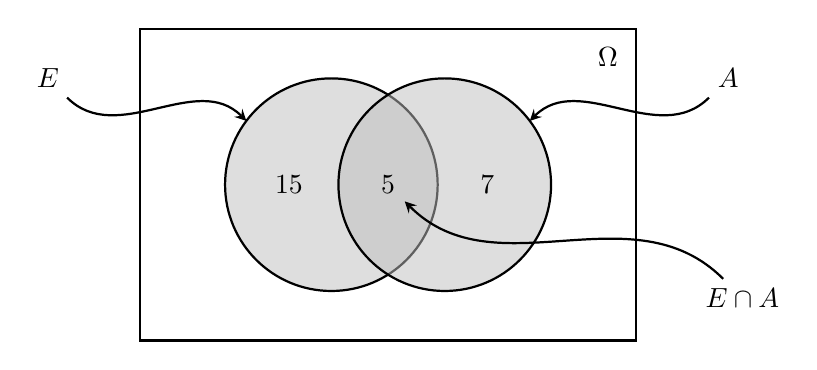
\begin{tikzpicture}[scale=0.9]
			\draw[thick, fill=white] (-3.5,-2.2) rectangle (3.5,2.2);
			\node at (3.1,1.8) {$\Omega$};
			\draw[thick, fill=gray!50, fill opacity=0.5] (-0.8,0) circle (1.5);
			\draw[thick, fill=gray!50, fill opacity=0.5] (0.8,0) circle (1.5);
			\node at (-1.4,0) {$15$};
			\node (inter) at (0,0) {$5$};
			\node at (1.4,0) {$7$};
			\node (nodeE) at (-4.8,1.5) {\textbf{$E$}};
			\draw[->, >=stealth, thick] (nodeE) to[out=-45, in=135] (-2,0.9);
			\node (nodeA) at (4.8,1.5) {\textbf{$A$}};
			\draw[->, >=stealth, thick] (nodeA) to[out=-135, in=45] (2,0.9);
			\node (nodeInter) at (5,-1.6) {\textbf{$E \cap A$}};
			\draw[->, >=stealth, thick] (nodeInter) to[out=135, in=-45] (inter);
		\end{tikzpicture}
	\end{center}

	On choisit un élève au hasard.

	Grâce au diagramme, on lit directement la répartition des effectifs disjoints~:
	\begin{itemize}
		\item Probabilité que l'élève étudie l'Espagnol \textbf{et} l'Allemand~:
		      \[ P(E \cap A) = \dfrac{\text{Card}(E \cap A)}{\text{Card}(\Omega)} = \dfrac{5}{35} = \dfrac{1}{7} \]
		\item Probabilité que l'élève étudie \textbf{uniquement} l'Espagnol~:
		      \[ P(E \setminus A) = \dfrac{20 - 5}{35} = \dfrac{15}{35} = \dfrac{3}{7} \]
		\item Probabilité que l'élève étudie \textbf{au moins une} des deux langues~:
		      \[ P(E \cup A) = \dfrac{15 + 5 + 7}{35} = \dfrac{27}{35} \]
		\item Probabilité que l'élève n'étudie \textbf{aucune} de ces deux langues~:
		      \[ P\pa{\bar{E \cup A}} = 1 - P(E \cup A) = 1 - \dfrac{27}{35} = \dfrac{8}{35} \]
	\end{itemize}
\end{ex}

% \chapter{Probabilité conditionnelle}

\section{Calcul à l'aide d'un tableau croisé}

\subsection{Tableau d'effectifs et de fréquences}

Dans une étude statistique portant sur deux caractères, on organise souvent les données dans un tableau croisé à double entrée (ou tableau d'effectifs).

\begin{ex}
	On a interrogé $200$ personnes sur leur pratique sportive. Les résultats sont consignés ci-dessous :

	\begin{center}
		\def\arraystretch{1.5}
		\begin{tabular}{|l|c|c|c|} \hline
			                                & \textbf{Sportif $\pa{S}$} & \textbf{Non-sportif $\pa{\bar{S}}$} & \textbf{Total} \\ \hline
			\textbf{Jeunes $\pa{J}$}        & $45$                      & $15$                                & \textbf{60}    \\ \hline
			\textbf{Adultes $\pa{\bar{J}}$} & $80$                      & $60$                                & \textbf{140}   \\ \hline
			\textbf{Total}                  & \textbf{125}              & \textbf{75}                         & \textbf{200}   \\ \hline
		\end{tabular}
	\end{center}

	\begin{itemize}
		\item \textbf{Effectif total :} $\text{Card}(\Omega) = 200$ personnes.
		\item \textbf{Effectif de l'intersection :} $\text{Card}(J \cap S) = 45$ personnes sont à la fois \og{}Jeunes\fg{} \textbf{et} \og{}Sportifs\fg{}.
		\item \textbf{Effectifs marginaux :} $\text{Card}(J) = 60$ personnes sont jeunes ; $\text{Card}(S) = 125$ personnes sont sportives.
	\end{itemize}
\end{ex}

\begin{defin}[Fréquences marginales et conditionnelles]
	Soit un tableau d'effectifs croisant deux caractères :
	\begin{itemize}
		\item Une \textbf{fréquence marginale} est la fréquence d'un caractère calculée par rapport à l'effectif total.

		      Elle se lit dans les marges du tableau.
		\item Une \textbf{fréquence conditionnelle} est la fréquence d'un caractère calculée en se restreignant à une ligne ou une colonne précise (sous-population).
	\end{itemize}
\end{defin}

\begin{methode}[Calculer des fréquences conditionnelles]
	En reprenant l'exemple précédent :
	\begin{enumerate}
		\item La fréquence marginale des jeunes est :
		      \[
			      f_J = \dfrac{60}{200} = 0,30 = 30\%
		      \]
		\item La fréquence conditionnelle des sportifs parmi les jeunes se calcule en se limitant à la ligne \og{}Jeunes\fg{} :
		      \[
			      f_{\text{sportif sachant jeune}} = \dfrac{45}{60} = 0,75 = 75\%
		      \]
		\item La fréquence conditionnelle des jeunes parmi les sportifs se calcule en se limitant à la colonne \og{}Sportif\fg{} :
		      \[
			      f_{\text{jeune sachant sportif}} = \dfrac{45}{125} = 0,36 = 36\%
		      \]
	\end{enumerate}
\end{methode}

\section{Probabilités conditionnelles}

\subsection{Définition et calculs}

\begin{defin}[Probabilité conditionnelle]
	Soit $A$ un événement de probabilité non nulle.

	On appelle \textbf{probabilité conditionnelle} de $B$ sachant $A$, la probabilité que l'événement $B$ se réalise sachant que l'événement $A$ est réalisé.

	Elle se note $P_A(B)$.
\end{defin}

\begin{ex}
	On considère l'expérience aléatoire qui consiste à \textbf{choisir une personne au hasard} parmi les $200$ personnes interrogées dans l'étude précédente.

	L'univers $\Omega$ est l'ensemble de ces $200$ personnes ($\text{Card}(\Omega) = 200$).

	On définit les événements suivants :

	\begin{itemize}
		\item $J$ : \og{}La personne choisie est jeune\fg{} ;
		\item $S$ : \og{}La personne choisie est sportive\fg{}.
	\end{itemize}

	On a donc :

	\begin{itemize}
		\item $P(S)$ est la probabilité qu'une personne prise au hasard dans \textbf{toute la population} soit sportive ($125$ personnes sur $200$).
		\item $P_J(S)$ est la probabilité qu'une personne soit sportive \textbf{sachant qu'elle fait partie des jeunes}.

		      On ne regarde plus tout le monde, on se focalise uniquement sur le groupe des jeunes ($45$ sportifs sur les $60$ jeunes).
	\end{itemize}
\end{ex}

\begin{prop}[Calculs de probabilités conditionnelles]
	Pour tout événement $A$ tel que $P(A) \neq 0$ :
	\begin{itemize}
		\item \textbf{Formule générale :}
		      \[
			      P_A(B) = \dfrac{P(A \cap B)}{P(A)}
		      \]
		\item \textbf{Lien avec les effectifs (équiprobabilité) :}
		      \[
			      P_A(B) = \dfrac{\text{Card}(A \cap B)}{\text{Card}(A)}
		      \]
	\end{itemize}
\end{prop}

\begin{methode}[Calculer une probabilité conditionnelle à partir d'un tableau]
	Un laboratoire pharmaceutique réalise une étude sur 800 patients :

	\begin{center}
		\def\arraystretch{1.5}
		\begin{tabular}{|l|c|c|c|} \hline
			                                  & \textbf{Médicament A} & \textbf{Médicament B} & \textbf{Total} \\ \hline
			\textbf{Guéri $\pa{G}$}           & $383$                 & $291$                 & $674$          \\ \hline
			\textbf{Non guéri $\pa{\bar{G}}$} & $72$                  & $54$                  & $126$          \\ \hline
			\textbf{Total}                    & $455$                 & $345$                 & $800$          \\ \hline
		\end{tabular}
	\end{center}

	On choisit un patient au hasard.
	\begin{enumerate}
		\item Probabilité que le patient soit guéri : $P(G) = \dfrac{674}{800} = 0,8425$.
		\item Probabilité que le patient ait pris le médicament A sachant qu'il est guéri :
		      \[
			      P_G(A) = \dfrac{\text{Card}(A \cap G)}{\text{Card}(G)} = \dfrac{383}{674} \approx 0,568
		      \]
	\end{enumerate}
\end{methode}

\section{Représentation par un arbre pondéré}

\subsection{Construction et règles de lecture}

Un arbre pondéré permet de modéliser une succession d'épreuves.

\begin{center}
	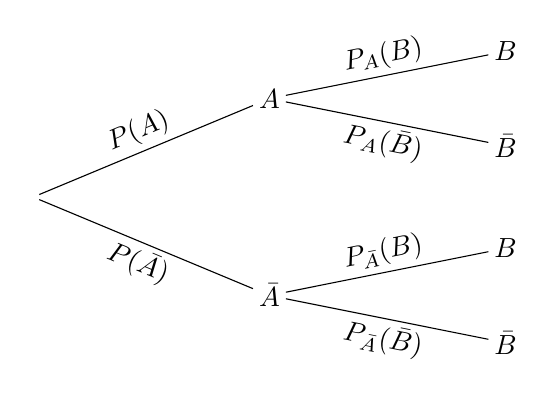
\begin{tikzpicture}[
			grow=right,
			level 1/.style={level distance=3cm, sibling distance=2.5cm},
			level 2/.style={level distance=3cm, sibling distance=1.2cm},
			every node/.style={inner sep=2pt}
		]
		\node {}
		child { node { $\bar{A}$ }
				child { node { $\bar{B}$ } edge from parent node[sloped, below] { $P_{\bar{A}}(\bar{B})$ } }
				child { node { $B$ } edge from parent node[sloped, above] { $P_{\bar{A}}(B)$ } }
				edge from parent node[sloped, below] { $P(\bar{A})$ }
			}
		child { node { $A$ }
				child { node { $\bar{B}$ } edge from parent node[sloped, below] { $P_A(\bar{B})$ } }
				child { node { $B$ } edge from parent node[sloped, above] { $P_A(B)$ } }
				edge from parent node[sloped, above] { $P(A)$ }
			};
	\end{tikzpicture}
\end{center}

\begin{ex}
	On choisit un élève au hasard dans un lycée et on note :
	\begin{itemize}
		\item $F$ : \og{}L'élève est une fille\fg{}
		\item $L$ : \og{}L'élève a les cheveux longs\fg{}
	\end{itemize}

	On suppose que le lycée compte $45\%$ de filles.

	Dans ce lycée :
	\begin{itemize}
		\item $60\%$ des filles ont les cheveux longs ($P_F(L) = 0{,}6$) ;
		\item $20\%$ des garçons ont les cheveux longs ($P_{\bar{F}}(L) = 0{,}2$).
	\end{itemize}

	\begin{center}
		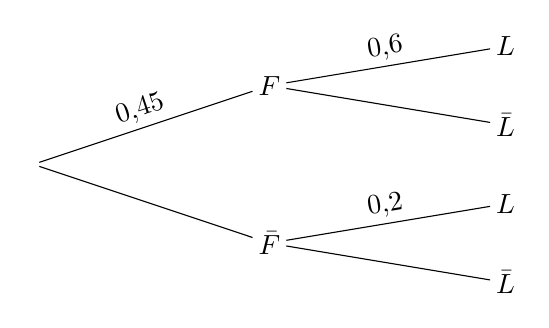
\begin{tikzpicture}[
				grow=right,
				level 1/.style={level distance=3cm, sibling distance=2cm},
				level 2/.style={level distance=3cm, sibling distance=1cm},
				every node/.style={inner sep=2pt}
			]
			\node {}
			child { node { $\bar{F}$ }
					child { node { $\bar{L}$ } edge from parent node[sloped, below] {  } }
					child { node { $L$ } edge from parent node[sloped, above] { $0{,}2$ } }
					edge from parent node[sloped, below] {  }
				}
			child { node { $F$ }
					child { node { $\bar{L}$ } edge from parent node[sloped, below] {  } }
					child { node { $L$ } edge from parent node[sloped, above] { $0{,}6$ } }
					edge from parent node[sloped, above] { $0{,}45$ }
				};
		\end{tikzpicture}
	\end{center}
\end{ex}

\begin{prop}[Règles des n\oe{}uds]
	\nline
	\begin{wrapstuff}[r]
		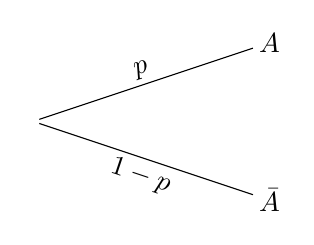
\begin{tikzpicture}[ grow=right, level 1/.style={level distance=3cm, sibling distance=2cm}, every node/.style={inner sep=2pt} ]
			\node {}
			child { node { $\bar{A}$ } edge from parent node[sloped, below] { $1-p$ } }
			child { node { $A$ } edge from parent node[sloped, above] { $p$ } };
		\end{tikzpicture}
	\end{wrapstuff}

	La somme des probabilités des branches issues d'un même n\oe{}ud est égale à 1.
	\[
		P(A) + P(\bar{A}) = 1 \quad \text{et} \quad P_A(B) + P_A(\bar{B}) = 1
	\]

	\phantom{x}

	\phantom{x}
\end{prop}

\begin{prop}[Probabilité d'une intersection]
	\nline
	\begin{wrapstuff}[r]
		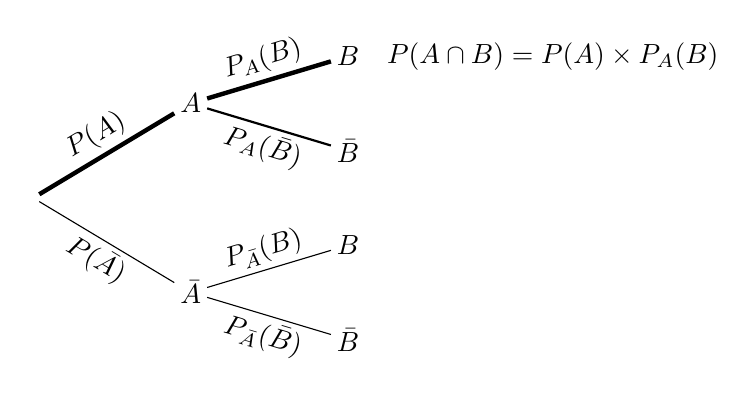
\begin{tikzpicture}[
				grow=right,
				level 1/.style={level distance=2cm, sibling distance=2.4cm},
				level 2/.style={level distance=2cm, sibling distance=1.2cm},
				every node/.style={inner sep=2pt}
			]
			\node {}
			child { node { $\bar{A}$ }
					child { node { $\bar{B}$ } edge from parent node[sloped, below] { $P_{\bar{A}}(\bar{B})$ } }
					child { node { $B$ } edge from parent node[sloped, above] { $P_{\bar{A}}(B)$ } }
					edge from parent node[sloped, below] { $P(\bar{A})$ }
				}
			child { node { $A$ }
					child { node { $\bar{B}$ } edge from parent[thick] node[sloped, below] { $P_A(\bar{B})$ } }
					child { node { $B$ }
							node[right=0.3cm] {$\rarr\  P(A \cap B) = P(A) \times P_A(B)$}
							edge from parent[ultra thick] node[sloped, above] { $P_A(B)$ }
						}
					edge from parent[ultra thick] node[sloped, above] { $P(A)$ }
				};
		\end{tikzpicture}
	\end{wrapstuff}
	La probabilité de l'événement situé au bout d'un chemin est le produit des probabilités rencontrées sur ce chemin.
	\[
		P(A \cap B) = P(A) \times P_A(B)
	\]

	\phantom{x}

	\phantom{x}

	\phantom{x}

	\phantom{x}
\end{prop}

\begin{ex}[Calcul d'une intersection et règle des n\oe{}uds]
	On reprend l'exemple de la répartition des élèves selon le sexe et la longueur des cheveux :
	\begin{center}
		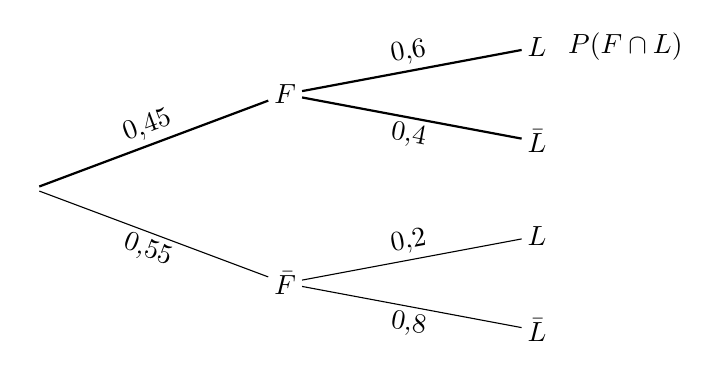
\begin{tikzpicture}[
				grow=right,
				level 1/.style={level distance=3.2cm, sibling distance=2.4cm},
				level 2/.style={level distance=3.2cm, sibling distance=1.2cm},
				every node/.style={inner sep=2pt}
			]
			\node {}
			child { node { $\bar{F}$ }
					child { node { $\bar{L}$ } edge from parent node[sloped, below] { $0{,}8$ } }
					child { node { $L$ } edge from parent node[sloped, above] { $0{,}2$ } }
					edge from parent node[sloped, below] { $0{,}55$ }
				}
			child { node { $F$ }
					child { node { $\bar{L}$ } edge from parent node[sloped, below] { $0{,}4$ } }
					child { node { $L$ }
							node[right=0.2cm] {$\rarr\ P(F \cap L)$}
							edge from parent[thick] node[sloped, above] { $0{,}6$ }
						}
					edge from parent[thick] node[sloped, above] { $0{,}45$ }
				};
		\end{tikzpicture}
	\end{center}

	\begin{enumerate}
		\item \textbf{Justification des valeurs manquantes (règle des n\oe{}uds) :}
		      \begin{itemize}
			      \item S'il y a $45\%$ de filles dans le lycée, alors le reste de la population est constitué de garçons, soit $55\%$.
			            \[
				            P(\bar{F}) = 1 - 0{,}45 = 0{,}55
			            \]
			      \item Si $60\%$ des filles ont les cheveux longs, alors les $40\%$ de filles restantes ont les cheveux courts :
			            \[
				            P_F(\bar{L}) = 1 - 0{,}6 = 0{,}4
			            \]
		      \end{itemize}

		\item \textbf{Calcul de la probabilité d'une intersection :}
		      Pour calculer la probabilité de choisir une fille aux cheveux longs, on multiplie les probabilités rencontrées le long du chemin passant par $F$ puis par $L$ :
		      \[
			      P(F \cap L) = P(F) \times P_F(L) = 0{,}45 \times 0{,}6 = 0{,}27
		      \]
		      Il y a donc $27\%$ de chances de choisir une fille aux cheveux longs dans ce lycée.
	\end{enumerate}
\end{ex}

\subsection{Formule des probabilités totales}

\begin{thm}[Formule des probabilités totales]
	Soit $A$ un événement et $\bar{A}$ son événement contraire. Pour tout événement $B$, sa probabilité est donnée par la somme des probabilités des chemins menant à $B$ :
	\[
		P(B) = P(A \cap B) + P(\bar{A} \cap B)
	\]

	Soit sous forme développée :
	\[
		P(B) = P(A) \times P_A(B) + P(\bar{A}) \times P_{\bar{A}}(B)
	\]

	\begin{center}
		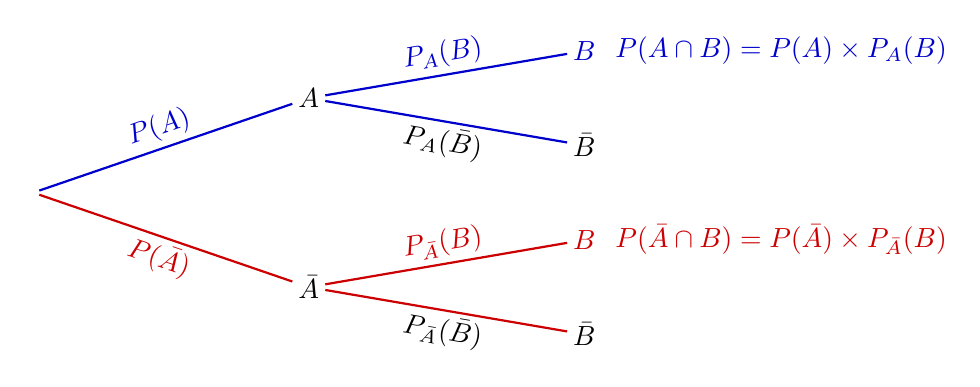
\begin{tikzpicture}[
				grow=right,
				level 1/.style={level distance=3.5cm, sibling distance=2.4cm},
				level 2/.style={level distance=3.5cm, sibling distance=1.2cm},
				every node/.style={inner sep=2pt}
			]
			\node {}
			child { node { $\bar{A}$ }
					child { node { $\bar{B}$ }
							edge from parent node[sloped, below] { $P_{\bar{A}}(\bar{B})$ }
						}
					child { node[red!80!black] { $B$ }
							node[right=0.2cm, red!80!black] {$\rarr\  P(\bar{A} \cap B) = P(\bar{A}) \times P_{\bar{A}}(B)$}
							edge from parent[red!80!black, thick] node[sloped, above] { $P_{\bar{A}}(B)$ }
						}
					edge from parent[red!80!black, thick] node[sloped, below] { $P(\bar{A})$ }
				}
			child { node { $A$ }
					child { node { $\bar{B}$ }
							edge from parent node[sloped, below] { $P_A(\bar{B})$ }
						}
					child { node[blue!80!black] { $B$ }
							node[right=0.2cm, blue!80!black] {$\rarr\  P(A \cap B) = P(A) \times P_A(B)$}
							edge from parent[blue!80!black, thick] node[sloped, above] { $P_A(B)$ }
						}
					edge from parent[blue!80!black, thick] node[sloped, above] { $P(A)$ }
				};
		\end{tikzpicture}
	\end{center}
\end{thm}

\newpage

\begin{methode}[Appliquer la formule des probabilités totales]
	Une maladie touche $2\%$ d'une population. Un test de dépistage donne les résultats suivants :
	\begin{itemize}
		\item Si un individu est malade $\pa{M}$, le test est positif $\pa{T}$ dans $85\%$ des cas.
		\item Si un individu est sain $\pa{\bar{M}}$, le test est négatif $\pa{\bar{T}}$ dans $95\%$ des cas.
	\end{itemize}

	\textbf{1. Modélisation par un arbre pondéré :}

	\begin{center}
		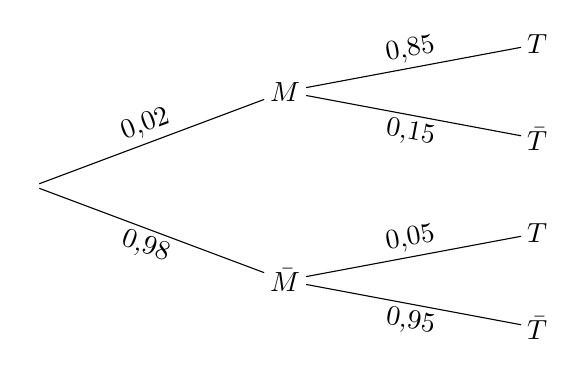
\begin{tikzpicture}[
				grow=right,
				level 1/.style={level distance=3.2cm, sibling distance=2.4cm},
				level 2/.style={level distance=3.2cm, sibling distance=1.2cm},
				every node/.style={inner sep=2pt}
			]
			\node {}
			child { node { $\bar{M}$ }
					child { node { $\bar{T}$ } edge from parent node[sloped, below] { $0{,}95$ } }
					child { node { $T$ } edge from parent node[sloped, above] { $0{,}05$ } }
					edge from parent node[sloped, below] { $0{,}98$ }
				}
			child { node { $M$ }
					child { node { $\bar{T}$ } edge from parent node[sloped, below] { $0{,}15$ } }
					child { node { $T$ } edge from parent node[sloped, above] { $0{,}85$ } }
					edge from parent node[sloped, above] { $0{,}02$ }
				};
		\end{tikzpicture}
	\end{center}

	\textbf{2. Calcul de la probabilité que le test soit positif $P(T)$ :}

	D'après la formule des probabilités totales :
	\[
		\begin{array}{rccccl}
			P(T) & = & P(M \cap T)        & + & P(\bar{M} \cap T)                &                         \\
			     & = & P(M) \times P_M(T) & + & P(\bar{M}) \times P_{\bar{M}}(T) &                         \\
			     & = & 0,02 \times 0,85   & + & 0,98 \times 0,05                 & = 0,017 + 0,049 = 0,066
		\end{array}
	\]

	La probabilité d'avoir un test positif est égale à $0,066$ (soit $6,6\%$).

	Dans les applications médicales, les probabilités conditionnelles liées à un test de dépistage portent des noms particuliers :

	\begin{itemize}
		\item \textbf{La sensibilité :} C'est la probabilité que le test soit positif sachant que l'individu est malade, soit :
		      \[
			      P_M(T) = 0{,}85
		      \]

		      Elle mesure la capacité du test à détecter la maladie.
		\item \textbf{La spécificité :} C'est la probabilité que le test soit négatif sachant que l'individu est sain, soit :
		      \[
				  P_{\bar{M}}\pa{\bar{T}} = 0{,}95
		      \]

		      Elle mesure la capacité du test à cibler uniquement les personnes malades.
	\end{itemize}
\end{methode}



% \part{Fonctions}
% \chapter{Généralités sur les fonctions}

\section{Définition, vocabulaire et notations}

\begin{defin}[Fonction et ensemble de définition]
	Soit $\mathcal{D}$ un intervalle ou une réunion d'intervalles de $\R$.

	Une \textbf{fonction} $f$ définie sur $\mathcal{D}$ associe à tout nombre réel $x \in \mathcal{D}$ un \textbf{unique} nombre réel, noté $f(x)$.

	$\mathcal{D}$ est l'\textbf{ensemble de définition} de la fonction $f$, parfois noté $\mathcal{D}_f$.

	On note :
	\[
		f : \begin{array}[t]{rcc}
			\mathcal{D} & \longrightarrow & \R   \\
			x           & \longmapsto     & f(x)
		\end{array}
	\]

	On lit : \og{}$f$ est la fonction qui, à $x$, associe $f(x)$\fg{}.
	\begin{center}
		\begin{tikzpicture}[scale=0.75,>=Stealth,ensemble/.style={draw, thick, minimum width=3cm, minimum height=1.8cm, rounded corners=5pt, align=center}]
			\node[ensemble, black] (DF) at (0,0) {};
			\node[ensemble, blue!30!black] (R) at (9,0) {};
			\node[black, above=3pt, font=\large\bfseries] at (DF.north) {$\mathcal{D}_f$};
			\node[blue!30!black, above=3pt, font=\large\bfseries] at (R.north) {$\R$};
			\coordinate (X) at ($(DF.center) + (0.3, 0.6)$);
			\coordinate (FX) at ($(R.center) - (0.3, -0.6)$);
			\fill (X) circle (2.5pt) node[left=3pt, font=\large] {$x$};
			\fill (FX) circle (2.5pt) node[right=3pt, font=\large] {$f(x)$};
			\draw[->, ultra thick, black!70] ($(DF.east) + (0.2, 0.6)$) -- ($(R.west) - (0.2, -0.6)$) node[midway, above=4pt, black, font=\huge\bfseries] {$f$};
			\node[font=\small, black] at (4.5, -0.2) {associe un \textbf{unique} réel};
			\node[below, black] at (DF.south) {Ensemble de départ};
			\node[below, black] at (R.south) {Ensemble d'arrivée};
		\end{tikzpicture}
	\end{center}
\end{defin}

\begin{rem}
	$x$ représente la \textbf{variable}. $f$ est le nom de la fonction (la \og{}machine\fg{} mathématique) tandis que $f(x)$ est un nombre réel (le résultat de la transformation).
\end{rem}

\begin{methode}[Déterminer un ensemble de définition]
	Pour déterminer l'ensemble de définition d'une fonction donnée par une expression algébrique, on recherche les éventuelles \textbf{valeurs interdites} :
	\begin{itemize}
		\item Un dénominateur ne doit jamais être nul.
		\item Une expression sous une racine carrée doit toujours être positive ou nulle.
	\end{itemize}

	Déterminer l'ensemble de définition des fonctions suivantes :

	\begin{multicols}{3}
		\begin{enumerate}
			\item $f(x) = 2x^2 - 3x + 1$
			\item $g(x) = \dfrac{x+4}{2x-6}$
			\item $h(x) = \sqrt{3x + 12}$
		\end{enumerate}
	\end{multicols}

	\begin{correction}
		\nline
		\begin{enumerate}
			\item $f(x)$ est définie pour tout réel $x$. Il n'y a ni fraction ni racine carrée. Ainsi, $\mathcal{D}_f = \R$.
			\item $g(x)$ existe si et seulement si son dénominateur n'est pas nul :
			      \[
				      2x - 6 = 0 \iff 2x = 6 \iff x = 3
			      \]
			      La valeur $3$ est une valeur interdite. Ainsi, $\mathcal{D}_g = \R \setminus \{3\} = \intoo{-\infty}{3} \cup \intoo{3}{+\infty}$.
			\item $h(x)$ existe si et seulement si la quantité sous la racine est supérieure ou égale à zéro :
			      \[
				      3x + 12 \ge 0 \iff 3x \ge -12 \iff x \ge -4
			      \]
			      Ainsi, $\mathcal{D}_h = \intfo{-4}{+\infty}$.
		\end{enumerate}
	\end{correction}
\end{methode}

\section{Images et antécédents}

\begin{defin}[Image et antécédent]
	Soit $f$ une fonction définie sur $\mathcal{D}$ et $a \in \mathcal{D}$.
	\begin{itemize}
		\item Le nombre $f(a)$ est l'\textbf{image} de $a$ par la fonction $f$.
		\item Si $f(a) = b$, on dit que $a$ est un \textbf{antécédent} de $b$ par la fonction $f$.
	\end{itemize}
\end{defin}

\begin{rem}
	\nline
	\begin{itemize}
		\item Un élément $x$ de $\mathcal{D}$ possède \textbf{une unique image} par $f$.
		\item Un nombre réel $b$ peut posséder \textbf{aucun}, \textbf{un} ou \textbf{plusieurs antécédents} par $f$.
	\end{itemize}
\end{rem}

\begin{methode}[Calculer une image et déterminer des antécédents]
	Soit $f$ la fonction définie sur $\R$ par $f(x) = x^2 - 2x - 3$.
	\begin{enumerate}
		\item Calculer l'image de $-2$ par $f$.
		\item Déterminer les antécédents éventuels de $-3$ par $f$.
	\end{enumerate}

	\begin{correction}
		\nline
		\begin{itemize}
			\item On remplace $x$ par $-2$ dans l'expression :
			      \[
				      f(-2) = (-2)^2 - 2 \times (-2) - 3 = 4 + 4 - 3 = 5
			      \]
			      L'image de $-2$ par $f$ est $5$.

			\item Chercher les antécédents de $-3$ revient à résoudre l'équation $f(x) = -3$ dans $\R$ :
			      \[
				      x^2 - 2x - 3 = -3 \iff x^2 - 2x = 0 \iff x(x - 2) = 0
			      \]

			      Un produit de facteurs est nul si et seulement si l'un au moins des facteurs est nul.
			      \[
				      x = 0 \quad \text{ou} \quad x - 2 = 0 \iff x = 2
			      \]
			      Les antécédents de $-3$ par $f$ sont $0$ et $2$.
		\end{itemize}
	\end{correction}
\end{methode}

\section{Représentation graphique}

\begin{defin}[Courbe représentative]
	Dans le plan muni d'un repère $\vOIJ$, la \textbf{courbe représentative} $\Cf$ d'une fonction $f$ définie sur $\mathcal{D}$ est l'ensemble des points $M(x\,;\,y)$ tels que :
	\[
		x \in \mathcal{D} \quad \text{et} \quad y = f(x)
	\]

	L'équation $y = f(x)$ est appelée \textbf{équation cartésienne} de la courbe $\Cf$.
\end{defin}

\begin{methode}[Appartenance d'un point à une courbe]
	Soit $f$ définie sur $\R$ par $f(x) = 3x - x^2$.

	Le point $A\coordl{-2}{-10}$ appartient-il à la courbe $\Cf$ ?

	\begin{correction}
		On a :
		\[
			A\coordl{x_A}{y_A} \in \Cf \iff f(x_A) = y_A
		\]

		On calcule $f(-2)$ :
		\[
			f(-2) = 3 \times (-2) - (-2)^2 = -6 - 4 = -10
		\]

		Comme $f(-2) = y_A$, le point $A\coordl{-2}{-10}$ appartient bien à la courbe $\Cf$.
	\end{correction}
\end{methode}

\begin{methode}[Lecture graphique d'images et d'antécédents]
	On considère la fonction $f$ représentée ci-dessous sur $\intff{-3}{4}$.

	\begin{center}
		\begin{tikzpicture}
			\clip (-2.5,-1.5) rectangle (4.5,4.5);
			\draw[very thin, black!20!white,step=0.25] (-3.5,-2.5) grid (4.5,4.5);
			\draw[thin,black!40!white] (-3.5,-2.5) grid (4.5,4.5);
			\foreach \x in {-3,-2,-1,1,2,3,4} \node[below=1pt, font=\small, black, fill=white] at (\x,0) {\x};
			\foreach \y in {-2,-1,1,2,3,4} \node[left=1pt, font=\small, black, fill=white] at (0,\y) {\y};
			\draw[-{Stealth}, black, thick] (-3.5,0) -- (4.5,0) node[right] {$x$};
			\draw[-{Stealth}, black, thick] (0,-2.5) -- (0,4.5) node[above] {$y$};
			\node[below left, font=\small] at (0,0) {0};
			\draw[blue!80!black, ultra thick, samples=100, domain=-3:4] plot(\x, {0.25*\x*\x*\x - 0.75*\x*\x - 0.25*\x + 2.75}) node[above left] {$\Cf$};
			\draw[dashed, green!30!black, thick] (2,0) -- (2,1.25) -- (0,1.25);
			\filldraw[green!30!black] (2,1.25) circle (2.5pt);
			\draw[dashed, red!50!black, very thick] (-3.5,2) -- (4.5,2);
			\draw[dashed, red!50!black, very thick] (-1,0) -- (-1,2);
			\draw[dashed, red!50!black, very thick] (1,0) -- (1,2);
			\draw[dashed, red!50!black, very thick] (3,0) -- (3,2);
			\filldraw[red!50!black] (-1,2) circle (2.5pt);
			\filldraw[red!50!black] (1,2) circle (2.5pt);
			\filldraw[red!50!black] (3,2) circle (2.5pt);
		\end{tikzpicture}
	\end{center}

	\begin{enumerate}
		\item Déterminer graphiquement l'image de $2$ par $f$.
		\item Déterminer les antécédents de $2$ par $f$.
	\end{enumerate}

	\begin{correction}
		\nline
		\begin{enumerate}
			\item On repère $2$ sur l'axe des abscisses, on rejoint la courbe verticalement puis on lit l'ordonnée.

			      L'image de $2$ par $f$ est $1.25$, soit $f(2) = 1.25$.

			\item On trace la droite horizontale $y = 2$. Elle coupe $\Cf$ en trois points.

			      Leurs abscisses sont les antécédents de $2$.

			      Les antécédents de $2$ sont $-1$ ; $1$ et $3$.
		\end{enumerate}
	\end{correction}
\end{methode}

\section{Parité d'une fonction}

\begin{defin}[Ensemble symétrique]
	Un ensemble de définition $\mathcal{D}$ est dit \textbf{symétrique par rapport à $0$} si pour tout $x \in \mathcal{D}$, on a $-x \in \mathcal{D}$.
\end{defin}

\begin{defin}[Fonctions paires et impaires]
	Soit $f$ une fonction définie sur un ensemble $\mathcal{D}$ symétrique par rapport à $0$.
	\begin{itemize}
		\item $f$ est \textbf{paire} si pour tout $x \in \mathcal{D}$, $f(-x) = f(x)$.
		\item $f$ est \textbf{impaire} si pour tout $x \in \mathcal{D}$, $f(-x) = -f(x)$.
	\end{itemize}
\end{defin}

\begin{prop}[Interprétation géométrique]
	Dans un repère orthogonal :
	\begin{itemize}
		\item La courbe d'une fonction \textbf{paire} est \textbf{symétrique par rapport à l'axe des ordonnées}.
		\item La courbe d'une fonction \textbf{impaire} est \textbf{symétrique par rapport à l'origine $O$}.
	\end{itemize}
\end{prop}

\begin{center}
	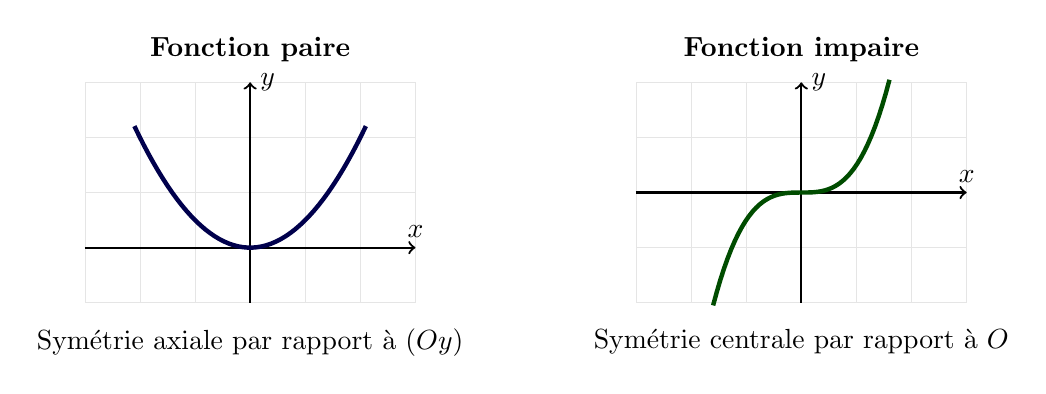
\begin{tikzpicture}[scale=0.7]
		\begin{scope}[xshift=-5cm]
			\draw[very thin, gray!20] (-3,-1) grid (3,3);
			\draw[->, thick] (-3,0) -- (3,0) node[above] {$x$};
			\draw[->, thick] (0,-1) -- (0,3) node[right] {$y$};
			\draw[blue!30!black, ultra thick, domain=-2.1:2.1, samples=50] plot(\x, {0.5*\x*\x});
			\node[above] at (0, 3.2) {\textbf{Fonction paire}};
			\node[below] at (0,-1.3) {Symétrie axiale par rapport à $(Oy)$};
		\end{scope}

		\begin{scope}[xshift=5cm,yshift=1cm]
			\draw[very thin, gray!20] (-3,-2) grid (3,2);
			\draw[->, thick] (-3,0) -- (3,0) node[above] {$x$};
			\draw[->, thick] (0,-2) -- (0,2) node[right] {$y$};
			\draw[green!30!black, ultra thick, domain=-1.6:1.6, samples=50] plot(\x, {0.5*\x*\x*\x});
			\node[above] at (0, 2.2) {\textbf{Fonction impaire}};
			\node[below] at (0,-2.3) {Symétrie centrale par rapport à $O$};
		\end{scope}
	\end{tikzpicture}
\end{center}

\newpage

\begin{methode}[Étudier la parité d'une fonction]
	Étudier la parité des fonctions définies sur $\R$ :
	\begin{multicols}{3}
		\begin{itemize}
			\item $f(x) = x^4 - 3x^2$
			\item $g(x) = \dfrac{2x}{x^2 + 1}$
		\end{itemize}
	\end{multicols}

	\begin{correction}
		\nline
		\begin{itemize}
			\item $\R$ est symétrique par rapport à $0$. Pour tout $x \in \R$ :
			      \[
				      f(-x) = (-x)^4 - 3(-x)^2 = x^4 - 3x^2 = f(x)
			      \]

			      La fonction $f$ est donc \textbf{paire}.
			\item $\R$ est symétrique par rapport à $0$. Pour tout $x \in \R$ :
			      \[
				      g(-x) = \dfrac{2(-x)}{(-x)^2 + 1} = \dfrac{-2x}{x^2 + 1} = -\pa{\dfrac{2x}{x^2 + 1}} = -g(x)
			      \]

			      La fonction $g$ est donc \textbf{impaire}.
		\end{itemize}
	\end{correction}
\end{methode}

\section{Variations et extrema}

\subsection{Sens de variation}

\begin{defin}[Croissance et décroissance]
	Soit $f$ une fonction définie sur un intervalle $I$.
	\begin{itemize}
		\item $f$ est \textbf{strictement croissante} sur $I$ si pour tous réels $a, b \in I$ tels que $a < b$, on a $f(a) < f(b)$.
		\item $f$ est \textbf{strictement décroissante} sur $I$ si pour tous réels $a, b \in I$ tels que $a < b$, on a $f(a) > f(b)$.
	\end{itemize}
\end{defin}

\begin{rem}
	\nline
	\begin{itemize}
		\item Une fonction \textbf{croissante} conserve l'ordre.
		\item Une fonction \textbf{décroissante} inverse l'ordre.
		\item Une fonction est dite \textbf{monotone} sur un intervalle $I$ si elle y est uniquement croissante ou uniquement décroissante.
	\end{itemize}
\end{rem}

\subsection{Extrema : Maximum et Minimum}

\begin{defin}[Maximum et minimum]
	Soit $f$ une fonction définie sur un intervalle $I$ et $x_0 \in I$.
	\begin{itemize}
		\item $f$ admet un \textbf{maximum} en $x_0$ sur $I$ si pour tout $x \in I$, $f(x) \le f(x_0)$. Ce maximum vaut $M = f(x_0)$.
		\item $f$ admet un \textbf{minimum} en $x_0$ sur $I$ si pour tout $x \in I$, $f(x) \ge f(x_0)$. Ce minimum vaut $m = f(x_0)$.
	\end{itemize}
\end{defin}

\subsection{Tableau de variations}

Un \textbf{tableau de variations} résume le sens de variation de la fonction $f$ ainsi que ses extrema locaux et aux bornes.

\begin{methode}[Dresser et exploiter un tableau de variations]
	Soit la fonction $f$ définie sur $[-5\,;\,6]$ dont le tableau de variations est donné ci-dessous.

	\begin{center}
		\begin{tikzpicture}
			\tkzTabInit[lgt=1.5, espcl=1.8, deltacl=0.5]{$x$ /1, $f(x)$ /2}{$-5$, $-1$, $3$, $6$}
			\tkzTabVar{-/ $-4$, +/ $5$, -/ $-2$, +/ $1$}
		\end{tikzpicture}
	\end{center}

	\begin{enumerate}
		\item Donner le sens de variation de $f$.
		\item Déterminer le maximum et le minimum de $f$ sur $\intff{-5}{6}$.
		\item Comparer, si possible, $f(-4)$ et $f(-2)$.
	\end{enumerate}

	\begin{correction}
		\nline
		\begin{enumerate}
			\item $f$ est strictement croissante sur $\intff{-5}{-1}$ et $\intff{3}{6}$, et strictement décroissante sur $\intff{-1}{3}$.
			\item Le maximum absolu de $f$ est $5$, atteint en $x = -1$. Le minimum absolu est $-4$, atteint en $x = -5$.
			\item Sur $\intff{-5}{-1}$, les nombres $-4$ et $-2$ sont rangés dans l'ordre $-5 \le -4 < -2 \le -1$.

			      Comme $f$ est \textbf{strictement croissante} sur cet intervalle, elle conserve l'ordre :
			      \[
				      f(-4) < f(-2)
			      \]
		\end{enumerate}
	\end{correction}
\end{methode}

\section{Résolutions graphiques et positions relatives}

\subsection{Équations et inéquations de la forme $f(x) = k$ et $f(x) \ge k$}

\begin{prop}[Résolution graphique]
	Soit $f$ une fonction définie sur $\mathcal{D}$ de courbe $\Cf$, et $k \in \R$.
	\begin{itemize}
		\item Les solutions de l'équation $f(x) = k$ sont les \textbf{abscisses} des points d'intersection de la courbe $\Cf$ avec la droite horizontale d'équation $y = k$.
		\item Les solutions de l'inéquation $f(x) > k$ (resp. $f(x) < k$) sont les \textbf{abscisses} des points de la courbe $\Cf$ situés \textbf{strictement au-dessus} (resp. au-dessous) de la droite $y = k$.
	\end{itemize}
\end{prop}

\begin{methode}[Résoudre graphiquement $f(x) = k$ et $f(x) \ge k$]
	On considère la fonction $f$ représentée par sa courbe $\Cf$ ci-dessous.

	\begin{center}
		\begin{tikzpicture}[scale=0.75]
			\draw[very thin, gray!40] (-3.5,-2.5) grid (3.5,3.5);
			\draw[-{Stealth}, thick] (-3.5,0) -- (3.5,0) node[above] {$x$};
			\draw[-{Stealth}, thick] (0,-2.5) -- (0,3.5) node[right] {$y$};
			\foreach \x in {-3,-2,-1,1,2,3} \node[below=1pt, font=\small, fill=white] at (\x,0) {\x};
			\foreach \y in {-2,-1,1,2,3} \node[left=1pt, font=\small, fill=white] at (0,\y) {\y};
			\node[below left, font=\small] at (0,0) {0};
			\draw[blue, ultra thick, samples=100, domain=-3.2:3.2] plot(\x, {0.5*\x*\x - 2}) node[above right] {$\Cf$};
			\draw[red, thick] (-3.5,2) -- (3.5,2) node[right] {$y = 2$};
			\filldraw (-2.83,2) circle (2.5pt);
			\filldraw (2.83,2) circle (2.5pt);
			\draw[dashed, thick] (-2.83,0) -- (-2.83,2);
			\draw[dashed, thick] (2.83,0) -- (2.83,2);
		\end{tikzpicture}
	\end{center}

	Résoudre graphiquement sur $\intff{-3}{3}$ :

	\begin{enumerate}
		\item L'équation $f(x) = 2$.
		\item L'inéquation $f(x) \ge 2$.
	\end{enumerate}

	\begin{correction}
		\nline
		\begin{enumerate}
			\item On trace la droite horizontale d'équation $y = 2$.

			      Elle coupe la courbe $\Cf$ en deux points d'abscisses $-2{,}8$ et $2{,}8$.

			      L'ensemble des solutions de l'équation $f(x) = 2$ est :
			      \[
				      S = \{-2{,}8\,;\,2{,}8\}
			      \]

			\item Les solutions de l'inéquation $f(x) \ge 2$ sont les abscisses des points de la courbe $\Cf$ situés \textbf{au-dessus ou sur} la droite d'équation $y = 2$.

			      L'ensemble des solutions est :
			      \[
				      S = \intff{-3}{-2{,}8} \cup \intff{2{,}8}{3}
			      \]
		\end{enumerate}
	\end{correction}
\end{methode}

\subsection{Résolution de $f(x) = g(x)$ et position relative de deux courbes}

\begin{prop}[Comparaison de deux fonctions]
	Soit $f$ et $g$ deux fonctions de courbes représentatives $\Cf$ et $\Cg$.
	\begin{itemize}
		\item Les solutions de $f(x) = g(x)$ sont les \textbf{abscisses} des points d'intersection de $\Cf$ et $\Cg$.
		\item $\Cf$ est \textbf{au-dessus} de $\Cg$ sur un intervalle si et seulement si $f(x) \ge g(x)$, soit $f(x) - g(x) \ge 0$.
		\item $\Cf$ est \textbf{en dessous} de $\Cg$ sur un intervalle si et seulement si $f(x) \le g(x)$, soit $f(x) - g(x) \le 0$.
	\end{itemize}
\end{prop}

\begin{methode}[Résoudre graphiquement une inéquation du type $f(x) < g(x)$]
	\nline
	\begin{wrapstuff}[r]
		\begin{tikzpicture}[scale=0.85]
			\draw[very thin, black!40] (-1.5,-0.5) grid (4.5,6.5);
			\draw[-{Stealth}, black, thick] (-1.5,0) -- (4.5,0) node[right] {$x$};
			\draw[-{Stealth}, black, thick] (0,-0.5) -- (0,6.5) node[above] {$y$};
			\foreach \x in {-1,1,2,3} \node[below=1pt, font=\small, black, fill=white] at (\x,0) {\x};
			\foreach \y in {1,2,3,4,5,6} \node[left=1pt, font=\small, black, fill=white] at (0,\y) {\y};

			\draw[cyan!60!black, ultra thick, samples=100, domain=-1.3:2.2] plot(\x,{\x*\x+2}) node[below right] {$\Cf$};
			\draw[green!60!black, ultra thick, samples=100, domain=-0.7:3.7] plot(\x,{-\x*\x+3*\x+2}) node[right] {$\Cg$};

			\filldraw[red!30!black] (0,2) circle (2.5pt);
			\filldraw[red!30!black] (1.5,4.25) circle (2.5pt);

			\draw[dashed, red!30!black, thick] (0,0) -- (0,2);
			\draw[dashed, red!30!black, thick] (1.5,0) -- (1.5,4.25);
		\end{tikzpicture}
	\end{wrapstuff}

	On a représenté les courbes $\Cf$ et $\Cg$ des fonctions :

	\begin{itemize}
		\item $f(x) = x^2 + 2$
		\item $g(x) = -x^2 + 3x + 2$
	\end{itemize}

	Résoudre graphiquement $f(x) < g(x)$.

	\ms

	\noindent\textit{Correction :}

	L'inéquation $f(x) < g(x)$ correspond aux valeurs de $x$ pour lesquelles $\Cf$ est \textbf{strictement au-dessous} de $\Cg$.

	Les deux courbes se coupent aux points d'abscisses $x = 0$ et $x = 1{,}5$.

	$\Cf$ est située en dessous de $\Cg$ entre ces deux valeurs.

	L'ensemble des solutions est donc :
	\[
		S = \left] 0\,;\,1{,}5 \right[
	\]
\end{methode}

\subsection{Tableau de signes}

Le \textbf{tableau de signes} permet de déterminer sur quels intervalles une fonction est positive ($f(x) \ge 0$), négative ($f(x) \le 0$) ou s'annule ($f(x) = 0$).

\begin{methode}[Dresser un tableau de signes graphiquement]
	Dresser le tableau de signes de la fonction $h$ représentée ci-contre sur $\intff{-3{,}5}{2{,}2}$.
	\begin{center}
		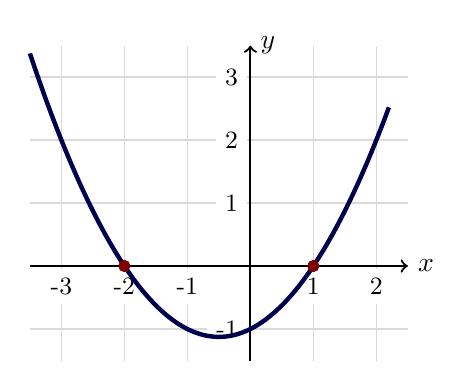
\begin{tikzpicture}[scale=0.80]
			\draw[thin, gray!30] (-3.5,-1.5) grid (2.5,3.5);
			\draw[->, thick] (-3.5,0) -- (2.5,0) node[right] {$x$};
			\draw[->, thick] (0,-1.5) -- (0,3.5) node[right] {$y$};
			\foreach \x in {-3,-2,-1,1,2} \node[below=1pt, font=\small, fill=white] at (\x,0) {\x};
			\foreach \y in {-1,1,2,3} \node[left=1pt, font=\small, fill=white] at (0,\y) {\y};
			\draw[blue!30!black, ultra thick, samples=100, domain=-3.5:2.2] plot (\x, {0.5*(\x+2)*(\x-1)});
			\filldraw[red!50!black] (-2,0) circle (2.5pt);
			\filldraw[red!50!black] (1,0) circle (2.5pt);
		\end{tikzpicture}
	\end{center}

	\begin{correction}
		$\mathcal{C}_h$ coupe l'axe des abscisses en $x = -2{,}7$ et $x = 0{,}7$.

		La courbe est au-dessus de l'axe sur $\intff{-3{,}5}{-2}$ et $\intff{1}{2{,}2}$, et au-dessous sur $\intff{-2}{1}$.
		\begin{center}
			\begin{tikzpicture}
				\tkzTabInit[lgt=1.5, espcl=1.8]{$x$ /1, $h(x)$ /1}{$-3{,}5$, $-2$, $1$, $2{,}2$}
				\tkzTabLine{, +, z, -, z, +, }
			\end{tikzpicture}
		\end{center}
	\end{correction}
\end{methode}

% \chapter{Variations et extremums de fonctions}

\section{Notions de croissance et de décroissance}

\subsection{Définitions}

\begin{defin}[Sens de variation]
	Soit $f$ une fonction définie sur un intervalle $I$.
	\begin{itemize}
		\item $f$ est \textbf{croissante} sur $I$ si pour tous réels $a$ et $b$ de $I$ tels que $a < b$, on a :
		      \[
			      f(a) \le f(b)
		      \]
		\item $f$ est \textbf{décroissante} sur $I$ si pour tous réels $a$ et $b$ de $I$ tels que $a < b$, on a :
		      \[
			      f(a) \ge f(b)
		      \]
	\end{itemize}
\end{defin}

\begin{ex}
	\nline
	\begin{itemize}
		\item \textbf{Illustration de la croissance sur $]0 \,;\, +\infty[$ :}

					      Pour la fonction $f: x \mapsto x^2$, si l'on choisit $a = 2$ et $b = 3$ (on a $a < b$), on constate que :
					      \[ f(2) = 2^2 =4\quad\text{ et }\quad f(3) = 3^2 \]

					      On observe que $f(2) < f(3)$ : l'ordre est conservé sur ces deux valeurs.

					      Cet exemple illustre le comportement de la fonction, mais pour \textbf{démontrer} qu'elle est croissante sur $]0 \,;\, +\infty[$, il faut le vérifier pour \textbf{tous} réels $a$ et $b$ tels que $0 < a < b$.

		\item \textbf{Illustration de la décroissance sur $]0 \,;\, +\infty[$ :}

		      Pour la fonction $g: x \mapsto \dfrac{1}{x}$, si l'on choisit $a = 2$ et $b = 4$ (on a $a < b$), on constate que :

		      \[
			      g(2) =\frac{1}{2}= 0{,}5\quad \text{ et }\quad g(4) = \frac{1}{4}=0{,}25
		      \]

		      On observe que $g(2) > g(4)$ : l'ordre est renversé pour ces deux valeurs.
	\end{itemize}
\end{ex}

\begin{rem}
	\nline
	\begin{itemize}
		\item Une fonction \textbf{croissante} \textbf{conserve l'ordre} des nombres et de leurs images.
		\item Une fonction \textbf{décroissante} \textbf{renverse l'ordre} des nombres et de leurs images.
		\item On parle de croissance ou décroissance \textbf{strictes} lorsque les inégalités sont strictes ($f(a) < f(b)$ ou $f(a) > f(b)$).
		\item Dire qu'une fonction est \textbf{monotone} sur un intervalle signifie qu'elle est soit uniquement croissante, soit uniquement décroissante sur cet intervalle.
	\end{itemize}
\end{rem}

\newpage

\begin{prop}[Interprétation graphique]
	\nline
	\begin{itemize}
		\item La courbe représentative d'une fonction croissante \textbf{monte} de la gauche vers la droite.
		\item La courbe représentative d'une fonction décroissante \textbf{descend} de la gauche vers la droite.
	\end{itemize}
	\begin{center}
		\begin{tikzpicture}[scale=0.9, >=Stealth]
			\begin{scope}
				\draw[->, thick] (-0.5,0) -- (4,0) node[right, font=\small] {$x$};
				\draw[->, thick] (0,-0.5) -- (0,3.5) node[above, font=\small] {$y$};
				\def\xa{0.8} \def\ya{0.75}
				\def\xb{3.2} \def\yb{2.55}
				\draw[thick, black, domain=0.2:3.8] plot (\x, {0.15*(\x+0.5)^2 + 0.5});
				\draw[dashed, gray] (\xa,0) node[below, black, font=\small] {$a$} -- (\xa,\ya) -- (0,\ya) node[left, black, font=\small] {$f(a)$};
				\draw[dashed, gray] (\xb,0) node[below, black, font=\small] {$b$} -- (\xb,\yb) -- (0,\yb) node[left, black, font=\small] {$f(b)$};
				\node[circle, fill=red!60!black, inner sep=1.5pt] at (\xa,\ya) {};
				\node[circle, fill=red!60!black, inner sep=1.5pt] at (\xb,\yb) {};
				\node[font=\small, black] at (1.75,-1) {$a < b \implies f(a) \le f(b)$};
			\end{scope}
			\begin{scope}[xshift=7cm]
				\draw[->, thick] (-0.5,0) -- (4,0) node[right, font=\small] {$x$};
				\draw[->, thick] (0,-0.5) -- (0,3.5) node[above, font=\small] {$y$};
				\def\xa{0.8} \def\ya{2.8465}
				\def\xb{3.2} \def\yb{1.06}
				\draw[thick, black, domain=0.2:3.8] plot (\x, {-0.15*(\x+0.5)^2 + 3.1});
				\draw[dashed, gray] (\xa,0) node[below, black, font=\small] {$a$} -- (\xa,\ya) -- (0,\ya) node[left, black, font=\small] {$f(a)$};
				\draw[dashed, gray] (\xb,0) node[below, black, font=\small] {$b$} -- (\xb,\yb) -- (0,\yb) node[left, black, font=\small] {$f(b)$};
				\node[circle, fill=red!60!black, inner sep=1.5pt] at (\xa,\ya) {};
				\node[circle, fill=red!60!black, inner sep=1.5pt] at (\xb,\yb) {};
				\node[font=\small, black] at (1.75,-1) {$a < b \implies f(a) \ge f(b)$};
			\end{scope}
		\end{tikzpicture}
	\end{center}
\end{prop}

\subsection{Extremums d'une fonction}

\begin{defin}[Maximum et Minimum]
	Soit $f$ une fonction définie sur un ensemble $D$.
	\begin{itemize}
		\item $f$ admet un \textbf{maximum} $M$ sur $D$, atteint en $a$, si pour tout $x \in D$ :
		      \[
			      f(x) \le M \quad \text{avec} \quad f(a) = M
		      \]
		\item $f$ admet un \textbf{minimum} $m$ sur $D$, atteint en $b$, si pour tout $x \in D$ :
		      \[
			      f(x) \ge m \quad \text{avec} \quad f(b) = m
		      \]
	\end{itemize}
	Un maximum ou un minimum est appelé un \textbf{extremum}.
\end{defin}

\begin{rem}
	Graphiquement, le maximum correspond à l'ordonnée du point le plus haut de la courbe, et le minimum à l'ordonnée du point le plus bas.
\end{rem}

\section{Tableau de variations}

\begin{defin}[Tableau de variations]
	Étudier les variations d'une fonction consiste à déterminer les intervalles sur lesquels elle est croissante ou décroissante. On résume ces comportements dans un \textbf{tableau de variations}.
\end{defin}

\begin{ex}
	Soit $f$ une fonction définie sur l'intervalle $[-3 \,;\, 6]$.
	
	On sait que :
	\begin{itemize}
		\item $f$ est strictement croissante sur $[-3 \,;\, 1]$, avec $f(-3) = -2$ et $f(1) = 5$ ;
		\item $f$ est strictement décroissante sur $[1 \,;\, 6]$, avec $f(6) = 0$.
	\end{itemize}

	On résume l'ensemble de ces informations dans le tableau de variations suivant :

	\begin{center}
		\begin{tikzpicture}
			\tkzTabInit[lgt=1.5, espcl=3]{$x$ / 0.75, $f(x)$ / 2}{$-3$, $1$, $6$}
			\tkzTabVar{-/ $-2$, +/ $5$, -/ $0$}
		\end{tikzpicture}
	\end{center}
\end{ex}

\newpage

\begin{methode}[Dresser un tableau de variations à partir d'une courbe]
	On considère la fonction $f$ représentée graphiquement ci-dessous :
	\begin{center}
		\begin{tikzpicture}[scale=0.8]
			\draw[very thin, gray!40] (-5.5,-4.5) grid (7.5,4.5);
			\draw[-{Stealth}, black] (-5.5,0) -- (7.5,0) node[above] {$x$};
			\draw[-{Stealth}, black] (0,-4.5) -- (0,4.5) node[right] {$y$};
			\foreach \x in {-5,...,-1,1,2,...,7} \node[below, font=\small, black] at (\x,0) {\x};
			\foreach \y in {-4,...,-1,1,2,...,4} \node[left, font=\small, black] at (0,\y) {\y};
			\draw[very thick] plot[smooth] coordinates {(-5,-2)(-4,-4)(-3,-2)(-2,0)(0,3.5)(1,2)(2,1.5)(3,0.8)(5,-3)(7,1)};
			\filldraw[red] (-5,-2) circle (0.1);
			\filldraw[red] (-4,-4) circle (0.1);
			\filldraw[red] (0,3.5) circle (0.1);
			\filldraw[red] (5,-3) circle (0.1);
			\filldraw[red] (7,1) circle (0.1);
			\node[black, font=\large] at (2,2) {$\mathcal{C}_f$};
		\end{tikzpicture}
	\end{center}

	\begin{enumerate}
		\item Préciser l'ensemble de définition $D_f$ de $f$.
		\item Décrire les variations de $f$.
		\item Identifier les extremums de $f$ sur son ensemble de définition.
		\item Dresser le tableau de variations synthétique.
		\item Comparer, en justifiant par les variations de $f$, les nombres $f(1)$ et $f(4)$.
		\item Peut-on comparer $f(-2)$ et $f(2)$ uniquement à l'aide des variations de $f$ ?
	\end{enumerate}

	\begin{correction}
		\nline
		\begin{enumerate}
			\item La fonction est définie pour $x \in [-5 \,;\, 7]$.
			\item $f$ est décroissante sur $[-5 \,;\, -4]$ et $[0 \,;\, 5]$, puis croissante sur $[-4 \,;\, 0]$ et $[5 \,;\, 7]$.
			\item Le maximum de $f$ est $3{,}5$ (atteint en $x = 0$) et son minimum est $-4$ (atteint en $x = -4$).
			\item Tableau de variations :
			      \ms
			      \begin{center}
				      \begin{tikzpicture}
					      \tkzTabInit[lgt=1.5, espcl=2]{$x$ / 0.75, $f(x)$ / 2}{$-5$, $-4$, $0$, $5$, $7$}
					      \tkzTabVar{+/ $-2$, -/ $-4$, +/ $3{,}5$, -/ $-3$, +/ $1$}
				      \end{tikzpicture}
			      \end{center}
		    \item Les nombres $1$ et $4$ appartiennent tous les deux à l'intervalle $[0 \,;\, 5]$ sur lequel la fonction $f$ est strictement décroissante.

		           Comme $1 < 4$, la fonction $f$ renverse l'ordre, d'où $f(1) > f(4)$.
		    \item Non. Le nombre $-2$ appartient à l'intervalle $[-4 \,;\, 0]$ où $f$ est croissante, tandis que $2$ appartient à l'intervalle $[0 \,;\, 5]$ où $f$ est décroissante.

				Les variations de la fonction sur deux intervalles distincts ne permettent pas de comparer leurs images directes sans information supplémentaire.
		\end{enumerate}
	\end{correction}
\end{methode}

% \chapter{Fonctions affines}

\section{Définitions et représentations graphiques}

\subsection{Fonctions affines, particulières et contre-exemples}

\begin{defin}[Fonction affine]
	Soit $f$ une fonction définie sur $\mathbb{R}$.

	$f$ est une \textbf{fonction affine} s'il existe deux réels $m$ et $p$ tels que, pour tout $x \in \mathbb{R}$ :

	\[
		f(x) = \textcolor{red}{m}x + \textcolor{blue}{p}
	\]

	Le réel $\textcolor{red}{m}$ est appelé le \textbf{coefficient directeur} (ou la pente) et $\textcolor{blue}{p}$ est l' \textbf{ordonnée à l'origine}.
\end{defin}

\begin{defin}[Cas particuliers]
	Soit $f(x) = mx + p$ une fonction affine :

	\begin{itemize}
		\item Si $p = 0$, $f(x) = mx$. La fonction $f$ est dite \textbf{linéaire}.

		      Elle traduit une situation de proportionnalité.
		\item Si $m = 0$, $f(x) = p$. La fonction $f$ est dite \textbf{constante}.
	\end{itemize}
\end{defin}

\begin{ex}
	\nline
	\begin{center}
		\def\arraystretch{1.5}
		\begin{tabular}{|l|c|c|l|} \hline
			\textbf{Fonction}                                                                & $\textcolor{red}{m}$ & $\textcolor{blue}{p}$ & \textbf{Nature}                \\ \hline
			$f(x) = 3x - 4$                                                                  & $3$                  & $-4$                  & Fonction affine                \\ \hline
			$g(x) = -x + 2$                                                                  & $-1$                 & $2$                   & Fonction affine                \\ \hline
			$h(x) = 5x$                                                                      & $5$                  & $0$                   & Fonction linéaire (et affine)  \\ \hline
			$k(x) = -7$                                                                      & $0$                  & $-7$                  & Fonction constante (et affine) \\ \hline
			\rule[-5mm]{0mm}{13mm}$l(x) = \dfrac{1 - 2x}{3} = -\dfrac{2}{3}x + \dfrac{1}{3}$ & $-\dfrac{2}{3}$      & $\dfrac{1}{3}$        & Fonction affine                \\ \hline
		\end{tabular}
	\end{center}
\end{ex}

\begin{rem}
	\textbf{Contre-exemples :} $x \mapsto x^2 + 1$, $x \mapsto \dfrac{2}{x}$ ou $x \mapsto \sqrt{x}$ ne sont pas des fonctions affines.
\end{rem}

\subsection{Représentation graphique}

\begin{prop}{}
	Dans un repère, la représentation graphique de la fonction affine $f(x) = mx + p$ est une \textbf{droite} non verticale, notée $\mathcal{D}_f$.
	\begin{itemize}
		\item Un point $M(x\,;\,y)$ appartient à $\mathcal{D}_f$ si et seulement si $y = f(x) = mx + p$.
		\item $p$ est l'ordonnée du point d'intersection de $\mathcal{D}_f$ avec l'axe des ordonnées : la droite passe par $(0\,;\,p)$.
		\item Si $f$ est linéaire ($p = 0$), la droite passe par l'origine $O(0\,;\,0)$.
		\item Si $f$ est constante ($m = 0$), la droite est horizontale.
	\end{itemize}
\end{prop}

\newpage

\begin{methode}[Lire graphiquement $m$ et $p$]
	\nline
	\begin{wrapstuff}[r]
		\begin{tikzpicture}[scale=0.8]
			\draw[very thin, gray!40] (-1.5,-2.5) grid (4.5,4.5);
			\draw[-{Stealth}, black, thick] (-1.5,0) -- (4.5,0) node[right] {$x$};
			\draw[-{Stealth}, black, thick] (0,-2.5) -- (0,4.5) node[above] {$y$};
			\foreach \x in {-1,1,2,3,4} \node[below, font=\tiny, black] at (\x,0) {\x};
			\foreach \y in {-2,-1,1,2,3,4} \node[left, font=\tiny, black] at (0,\y) {\y};
			\node[below left, font=\tiny] at (0,0) {0};
			\node[right=2pt, font=\small, fill=white, anchor=north west] at (0,-1) {$(0\,;\, - 1)$};
			\draw[blue, ultra thick, domain=-1.1:3.5] plot(\x,{1.5*\x - 1});
			\filldraw[blue] (0,-1) circle (2pt);
			\node[green!50!black, below, font=\small, fill=white] at (2,0.2) {$\Delta x = +2$} ;
			\draw[green!50!black, thick, dashed] (1,0.5) -- (3,0.5) -- (3,3.5);
			\draw[green!50!black, thick, <->] (1,0.2) -- (3,0.2);
			\draw[green!50!black, thick, <->] (3.2,0.5) -- node[right, font=\small, fill=white] {$\Delta y = +3$} (3.2,3.5);
			\node[above left, font=\small,fill=white] at (1,0.5) {$A(1\,;\,0{,}5)$};
			\filldraw[red] (1,0.5) circle (3pt);
			\node[above left, font=\small,fill=white] at (3,3.5) {$B(3\,;\,3{,}5)$};
			\filldraw[red] (3,3.5) circle (3pt);
		\end{tikzpicture}
	\end{wrapstuff}

	Pour lire l'expression de la fonction affine associée à la droite ci-contre :

	\begin{enumerate}
		\item \textbf{Ordonnée à l'origine :}

		      La droite coupe l'axe des ordonnées au point $(0\,;\, - 1)$, donc $\textcolor{blue}{p = -1}$.
		\item \textbf{Coefficient directeur :}

		      On choisit deux points $A(1\,;\,0{,}5)$ et $B(3\,;\,3{,}5)$.

		      En passant de $A$ à $B$, on avance de $\Delta x = 2$ et on monte de $\Delta y = 3$.

		      Ainsi :
		      \[
			      {m} = \frac{\Delta y}{\Delta x} = \frac{3{,}5 - 0{,}5}{3 - 1} = \frac{3}{2} = 1{,}5
		      \]
	\end{enumerate}

	On en déduit que :
	\[
		f(x) = 1{,}5x - 1
	\]
\end{methode}

\section{Propriétés analytiques et variations}

\subsection{Taux d'accroissement}

\begin{prop}[Taux d'accroissement]
	Soit $f$ une fonction affine $f(x) = mx + p$. Pour tous réels $a$ et $b$ distincts ($a \neq b$) :
	\[
		m = \frac{f(b) - f(a)}{b - a}
	\]

	Le coefficient directeur mesure \textbf{le taux de variation} constant de la fonction.
\end{prop}

\begin{methode}[Déterminer une fonction affine à partir de deux points ou images]
	Déterminer la fonction affine $f$ telle que $f(-1) = 3$ et $f(5) = 1$.

	\begin{correction}
		\nline
		\begin{enumerate}
			\item On calcule le coefficient directeur $m$ :
			      \[
				      \textcolor{red}{m} = \frac{f(5) - f(-1)}{5 - (-1)} = \frac{1 - 3}{5 + 1} = \frac{-2}{6} = \textcolor{red}{-\frac{1}{3}}
			      \]

			      Ainsi, $f(x) = \dfrac{-1}{3}x + p$.
			\item On détermine $p$ en utilisant l'une des deux images, par exemple $f(5) = 1$ :
			      \[
				      f(5) = 1 \iff -\frac{1}{3} \times 5 + p = 1 \iff -\frac{5}{3} + p = 1 \iff p = 1 + \frac{5}{3} = \textcolor{blue}{\frac{8}{3}}
			      \]
		\end{enumerate}

		L'expression cherchée est donc $f(x) = \dfrac{-1}{3}x + \dfrac{8}{3}$.
	\end{correction}
\end{methode}

\newpage

\subsection{Sens de variation}

\begin{prop}[Variations d'une fonction affine]
	Soit $f(x) = mx + p$ définie sur $\mathbb{R}$.
	\begin{itemize}
		\item Si $m > 0$, $f$ est \textbf{strictement croissante} sur $\mathbb{R}$.
		\item Si $m < 0$, $f$ est \textbf{strictement décroissante} sur $\mathbb{R}$.
		\item Si $m = 0$, $f$ est \textbf{constante} sur $\mathbb{R}$.
	\end{itemize}
\end{prop}

\begin{ex}[Variation d'une fonction affine]
	Soit $f(x) = -3x + 5$ définie sur $\mathbb{R}$.\par

	On a $m = -3 < 0$, donc $f$ est \textbf{strictement décroissante} sur $\mathbb{R}$.

	\begin{center}
		\begin{tikzpicture}
			\tkzTabInit[lgt=2, espcl=3]{$x$ / 0.5, $f(x)$ / 1}{$-\infty$, $+\infty$}
			\tkzTabVar{+ / , - / }
		\end{tikzpicture}
	\end{center}
\end{ex}

\subsection{Signe de $f(x) = mx + p$}

\begin{prop}[Tableau de signe]
	La fonction affine $f(x) = mx + p$ avec $m \neq 0$ s'annule en $x = \dfrac{-p}{m}$.

	Cette valeur est appelée la \textbf{racine} de la fonction.

	Son signe dépend du signe de son coefficient directeur $m$ (\textbf{signe de $m$ à droite du zéro}) :

	\begin{center}
		\def\arraystretch{1.5}
		\begin{tabular}{cc}
			Si $m > 0$ & Si $m < 0$ \\[4pt]
			\begin{tikzpicture}
				\tkzTabInit[lgt=1.5, espcl=2]{$x$/1, $f(x)$/1}{$-\infty$, $\frac{-p}{m}$, $+\infty$}
				\tkzTabLine{,-,z,+,}
			\end{tikzpicture}
			           &
			\begin{tikzpicture}
				\tkzTabInit[lgt=1.5, espcl=2]{$x$/1, $f(x)$/1}{$-\infty$, $\frac{-p}{m}$, $+\infty$}
				\tkzTabLine{,+,z,-,}
			\end{tikzpicture}
		\end{tabular}
	\end{center}
\end{prop}

\begin{meth}[Étude complète du signe]
	Déterminer le signe de $g(x) = -2x + 6$ sur $\mathbb{R}$.
	\begin{correction}
		\nline
		\begin{itemize}
			\item \textbf{Racine :}
			      \begin{align*}
				      g(x) = 0 & \iff -2x + 6 = 0 \\
				               & \iff -2x = -6    \\
				               & \iff x = 3
			      \end{align*}
			\item \textbf{Signe :}

			      $m = -2 < 0$, donc $g(x)$ est positive avant 3 puis négative après.
		\end{itemize}
		\begin{center}
			\begin{tikzpicture}
				\tkzTabInit[lgt=1.5, espcl=2]{$x$/1, $g(x)$/1}{$-\infty$, $3$, $+\infty$}
				\tkzTabLine{,+,z,-,}
			\end{tikzpicture}
		\end{center}
	\end{correction}
\end{meth}

\newpage

\section{Applications : Inéquations produit et quotient}

Le tableau de signe des fonctions affines permet de résoudre des inéquations plus complexes par la règle des signes.

\begin{methode}[Inéquation produit]
	Résoudre sur $\mathbb{R}$ l'inéquation $(3x - 1)(2 - x) \ge 0$.

	\begin{correction}
		\nline
		\begin{enumerate}
			\item \textbf{Recherche des racines :}
			      \begin{itemize}
				      \item $3x - 1 = 0 \iff x = \dfrac{1}{3}$ \quad (avec $m = 3 > 0$)
				      \item $2 - x = 0 \iff x = 2$ \quad (avec $m = -1 < 0$)
			      \end{itemize}
			\item \textbf{Tableau de signe synthétique :}
			      \begin{center}
				      \begin{tikzpicture}
					      \tkzTabInit[lgt=3.5, espcl=2]
					      {$x$/1, $3x - 1$/1, $2 - x$/1, $(3x - 1)(2 - x)$/1}
					      {$-\infty$, $\dfrac{1}{3}$, $2$, $+\infty$}
					      \tkzTabLine{,-,z,+,t,+,}
					      \tkzTabLine{,+,t,+,z,-,}
					      \tkzTabLine{,-,z,+,z,-,}
				      \end{tikzpicture}
			      \end{center}
			\item \textbf{Conclusion :} On cherche les valeurs où le produit est supérieur ou égal à 0.
			      \[
				      S = \intff{\frac{1}{3}}{2}
			      \]
		\end{enumerate}
	\end{correction}
\end{methode}

\begin{methode}[Inéquation quotient]
	Résoudre sur $\mathbb{R}$ l'inéquation $\dfrac{4x + 2}{1 - x} < 0$.

	\begin{correction}
		\nline
		\begin{enumerate}
			\item \textbf{Valeur interdite :} $1 - x = 0 \iff x = 1$. L'ensemble de définition est $\mathbb{R} \setminus \{1\}$.
			\item \textbf{Racine du numérateur :} $4x + 2 = 0 \iff x = -\dfrac{1}{2}$.
			\item \textbf{Tableau de signe (avec double barre pour la valeur interdite) :}
			      \begin{center}
				      \begin{tikzpicture}
					      \tkzTabInit[lgt=3.5, espcl=2]
					      {$x$/1, $4x + 2$/1, $1 - x$/1, $\dfrac{4x+2}{1-x}$/1}
					      {$-\infty$, $-\dfrac{1}{2}$, $1$, $+\infty$}
					      \tkzTabLine{,-,z,+,t,+,}
					      \tkzTabLine{,+,t,+,z,-,}
					      \tkzTabLine{,-,z,+,d,-,}
				      \end{tikzpicture}
			      \end{center}
			\item \textbf{Conclusion :} On cherche le signe strictement négatif ($< 0$).
			      \[
				      S = \left] -\infty\,;\, - \frac{1}{2} \right[\  \cup \ \left] 1\,;\, + \infty \right[
			      \]
		\end{enumerate}
	\end{correction}
\end{methode}



% \chapter{Fonctions de référence}

\section{Parité d'une fonction}

\begin{defin}[Fonction paire, fonction impaire]
	Soit $f$ une fonction définie sur un ensemble $D$ symétrique par rapport à $0$.
	\begin{itemize}
		\item $f$ est \textbf{paire} si, pour tout $x \in D$, $f(-x) = f(x)$.
		\item $f$ est \textbf{impaire} si, pour tout $x \in D$, $f(-x) = -f(x)$.
	\end{itemize}

	\begin{center}
		\begin{tikzpicture}[scale=0.8]
			% Paire
			\begin{scope}[xshift=-5.5cm]
				\draw[very thin, gray!40] (-2.9,-0.5) grid (2.9,4.5);
				\draw[-{Stealth}, black, thick] (-3,0) -- (3,0) node[right] {$x$};
				\draw[-{Stealth}, black, thick] (0,-0.5) -- (0,4.5) node[above] {$y$};
				\draw[blue, ultra thick, domain=-2.1:2.1, samples=60] plot(\x, {\x*\x});
				\draw[dashed, red, thick] (0,-0.5) -- (0,4.5);
				\node[below] at (0,-0.7) {Courbe symétrique par rapport à $(Oy)$};
				\node[below, font=\bfseries] at (0,-1.3) {Fonction paire};
			\end{scope}
			% Impaire
			\begin{scope}[xshift=5.5cm,yshift=2cm]
				\draw[very thin, gray!40] (-2.9,-2.5) grid (2.9,2.5);
				\draw[-{Stealth}, black, thick] (-3,0) -- (3,0) node[right] {$x$};
				\draw[-{Stealth}, black, thick] (0,-2.5) -- (0,2.5) node[above] {$y$};
				\draw[green!50!black, ultra thick, domain=-1.6:1.6, samples=60] plot(\x, {0.6*\x*\x*\x});
				\filldraw[red] (0,0) circle (2.5pt);
				\node[below] at (0,-2.7) {Courbe symétrique par rapport à $O$};
				\node[below, font=\bfseries] at (0,-3.3) {Fonction impaire};
			\end{scope}
		\end{tikzpicture}
	\end{center}
\end{defin}

\begin{methode}[Démontrer la parité d'une fonction]
	\nline
	\begin{enumerate}
		\item \textbf{Fonction paire :} Démontrer que $f(x) = 5x^2 + 3$ est paire sur $\mathbb{R}$.
		\item \textbf{Fonction impaire :} Démontrer que $g(x) = x^3 - 3x$ est impaire sur $\mathbb{R}$.
	\end{enumerate}

	\begin{correction}
		\nline
		\begin{enumerate}
			\item Pour tout $x \in \mathbb{R}$, $-x \in \mathbb{R}$ :
			      \[
				      f(-x) = 5(-x)^2 + 3 = 5x^2 + 3 = f(x)
			      \]
			      Donc $f$ est \textbf{paire}. Sa courbe est symétrique par rapport à l'axe des ordonnées.

			\item Pour tout $x \in \mathbb{R}$, $-x \in \mathbb{R}$ :
			      \[
				      g(-x) = (-x)^3 - 3(-x) = -x^3 + 3x = -(x^3 - 3x) = -g(x)
			      \]
			      Donc $g$ est \textbf{impaire}. Sa courbe est symétrique par rapport à l'origine $O$.
		\end{enumerate}
	\end{correction}
\end{methode}

\newpage

\section{Fonctions de référence}

\subsection{Fonction carré}

\begin{defin}[Fonction carré]
	La \textbf{fonction carré} est la fonction $f$ définie sur $\mathbb{R}$ par :
	\[
		f(x) = x^2
	\]
\end{defin}

\begin{prop}[Propriétés et variations]
	\nline
	\begin{itemize}
		\item Pour tout $x \in \mathbb{R}$, $x^2 \ge 0$.
		\item La fonction carré est \textbf{paire}.
		\item Elle est strictement décroissante sur $] - \infty\,;\,0]$ et strictement croissante sur $[0\,;\, + \infty[$.
	\end{itemize}

	\begin{center}
		\begin{tikzpicture}
			\tkzTabInit[lgt=2, espcl=3]{$x$ / 0.5, $x^2$ / 1.5}{$-\infty$, $0$, $+\infty$}
			\tkzTabVar{+ / $+\infty$, - / $0$, + / $+\infty$}
		\end{tikzpicture}
	\end{center}
\end{prop}

\begin{prop}[Représentation graphique]
	La représentation graphique de la fonction carré est une \textbf{parabole} de sommet $O(0\,;\,0)$, symétrique par rapport à l'axe des ordonnées.

	\begin{center}
		\begin{tikzpicture}[scale=0.9]
			\draw[very thin, gray!40] (-3.5,-0.5) grid (3.5,4.5);
			\draw[-{Stealth}, black, thick] (-3.5,0) -- (3.5,0) node[right] {$x$};
			\draw[-{Stealth}, black, thick] (0,-0.5) -- (0,4.5) node[above] {$y$};
			\foreach \x in {-3,-2,-1,1,2,3} \node[below, font=\small] at (\x,0) {$\x$};
			\foreach \y in {1,2,3,4} \node[left, font=\small] at (0,\y) {$\y$};
			\draw[blue, ultra thick, domain=-2.1:2.1, samples=80] plot(\x, {\x*\x});
			\filldraw (0,0) circle (3pt);
			\filldraw (-2,4) circle (3pt) (-1,1) circle (3pt) (1,1) circle (3pt) (2,4) circle (3pt);
		\end{tikzpicture}
	\end{center}
\end{prop}

\begin{methode}[Résolution de l'équation $x^2 = k$]
	Pour résoudre dans $\mathbb{R}$ l'équation $x^2 = k$ :
	\begin{itemize}
		\item Si $k > 0$, l'équation possède \textbf{deux solutions} : $x = \sqrt{k}$ et $x = -\sqrt{k}$.
		\item Si $k = 0$, l'équation possède \textbf{une unique solution} : $x = 0$.
		\item Si $k < 0$, l'équation ne possède \textbf{aucune solution} dans $\mathbb{R}$.
	\end{itemize}

	\begin{ex}
		Résoudre dans $\mathbb{R}$ l'équation $x^2 = 144$.

		\begin{correction}
			Comme $144 > 0$, l'équation admet deux solutions : $\begin{cases} x = \sqrt{144} = 12 \\ x = -\sqrt{144} = -12 \end{cases}$

			Ainsi, $S = \{-12\,;\,12\}$.
		\end{correction}
	\end{ex}
\end{methode}

\newpage

\subsection{Fonction racine carrée}

\begin{defin}[Fonction racine carrée]
	La \textbf{fonction racine carrée} est la fonction $f$ définie sur $[0\,;\, + \infty[$ par :
	\[
		f(x) = \sqrt{x}
	\]
\end{defin}

\begin{prop}[Variations et courbe]
	La fonction racine carrée est \textbf{strictement croissante} sur $[0\,;\, + \infty[$.

	Sa représentation graphique est une demi-parabole observée sur $[0\,;\, + \infty[$.

	\begin{center}
		\begin{tabular}{ccc}
			\begin{tikzpicture}[baseline=(current bounding box.center)]
				\tkzTabInit[lgt=1.8, espcl=2.5]{$x$ / 0.75, $\sqrt{x}$ / 1.5}{$0$, $+\infty$}
				\tkzTabVar{- / $0$, + /$+\infty$ }
			\end{tikzpicture}
			 & ~\hspace{2cm}~ &
			\begin{tikzpicture}[scale=0.8,baseline=(current bounding box.center)]
				\draw[very thin, gray!40] (-0.5,-0.5) grid (5.5,3.5);
				\draw[-{Stealth}, black, thick] (-0.5,0) -- (5.5,0) node[right] {$x$};
				\draw[-{Stealth}, black, thick] (0,-0.5) -- (0,3.5) node[above] {$y$};
				\foreach \x in {1,2,3,4,5} \node[below, font=\small] at (\x,0) {$\x$};
				\foreach \y in {1,2,3} \node[left, font=\small] at (0,\y) {$\y$};
				\draw[orange!90!black, ultra thick, domain=0:5.2, samples=100] plot(\x, {sqrt(\x)});
				\filldraw (0,0) circle (3pt);
				\filldraw (1,1) circle (3pt) (4,2) circle (3pt);
			\end{tikzpicture}
		\end{tabular}
	\end{center}
\end{prop}

\begin{methode}[Résoudre une équation de la forme $\sqrt{A(x)} = k$]
	Pour résoudre dans $\mathbb{R}$ l'équation $\sqrt{A(x)} = k$ :
	\begin{itemize}
		\item Si $k < 0$, l'équation n'a \textbf{aucune solution} ($S = \emptyset$) car une racine carrée est toujours positive ou nulle.
		\item Si $k \ge 0$, l'équation équivaut à $A(x) = k^2$, sous réserve que $A(x) \ge 0$.
	\end{itemize}
\end{methode}

\begin{ex}
	Résoudre dans $\mathbb{R}$ les équations :
	\begin{multicols}{3}
		\begin{enumerate}
			\item $\sqrt{x + 2} = -3$
			\item $\sqrt{2x - 1} = 5$
		\end{enumerate}
	\end{multicols}

	\begin{correction}
		\nline
		\begin{enumerate}
			\item Pour que la racine carrée soit définie, le terme sous la racine doit être supérieur ou égal à $0$ :
			      \[
				      x + 2 \ge 0 \iff x \ge -2
			      \]
			      Le membre de gauche est donc positif ou nul pour tout $x \ge -2$.

			      Or, le membre de droite est strictement négatif ($-3 < 0$).

			      Une racine carrée ne pouvant jamais être égale à un nombre négatif, l'équation n'a pas solution : $S = \emptyset$.

			\item Pour que la racine carrée soit définie, l'expression sous le radical doit être supérieur ou égal à $0$ :
			      \begin{align*}
				      2x - 1 \ge 0 & \iff 2x \ge 1          \\
				                   & \iff x \ge \frac{1}{2}
			      \end{align*}

			      Le membre de droite étant positif ($5 \ge 0$), on peut élever au carré sur l'intervalle $\left[ \dfrac{1}{2}\,;\, + \infty \right[$ :
			      \begin{align*}
				      \sqrt{2x - 1} = 5 & \iff 2x - 1 = 5^2 \\
				                        & \iff 2x - 1 = 25  \\
				                        & \iff 2x = 26      \\
				                        & \iff x = 13
			      \end{align*}

			      Comme $13 \ge \frac{1}{2}$, la solution est valide. Ainsi, $S = \brac{13}$.
		\end{enumerate}
	\end{correction}
\end{ex}

\newpage

\subsection{Fonction inverse}

\begin{defin}[Fonction inverse]
	La \textbf{fonction inverse} est la fonction $f$ définie sur $\mathbb{R} \setminus \{0\}$ (ou $\mathbb{R}^*$) par :
	\[
		f(x) = \dfrac{1}{x}
	\]
\end{defin}

\begin{prop}[Propriétés et variations]
	\nline
	\begin{itemize}
		\item La fonction inverse est \textbf{impaire}.
		\item Elle est \textbf{strictement décroissante} sur $] - \infty\,;\,0[$ et \textbf{strictement décroissante} sur $]0\,;\, + \infty[$.
	\end{itemize}

	\begin{center}
		\begin{tikzpicture}
			\tkzTabInit[lgt=2, espcl=2.5]{$x$ / 0.5, $\dfrac{1}{x}$ / 1.5}{$-\infty$, $0$, $+\infty$}
			\tkzTabVar{+ / $0$ , -D+ / $-\infty$ / $+\infty$ , - / $0$ }
		\end{tikzpicture}
	\end{center}
\end{prop}

\begin{prop}[Représentation graphique]
	La représentation graphique de la fonction inverse est une \textbf{hyperbole}, admettant l'origine $O(0\,;\,0)$ comme centre de symétrie.
	\begin{center}
		\begin{tikzpicture}[scale=0.8]
			\draw[very thin, gray!40] (-4.5,-3.5) grid (4.5,3.5);
			\draw[-{Stealth}, black, thick] (-4.5,0) -- (4.5,0) node[right] {$x$};
			\draw[-{Stealth}, black, thick] (0,-3.5) -- (0,3.5) node[above] {$y$};
			\foreach \x in {-4,-3,-2,-1,1,2,3,4} \node[below, font=\small] at (\x,0) {$\x$};
			\foreach \y in {-3,-2,-1,1,2,3} \node[left, font=\small] at (0,\y) {$\y$};
			\draw[magenta, ultra thick, domain=-4.2:-0.30, samples=100] plot(\x, {1/\x});
			\draw[magenta, ultra thick, domain=0.30:4.2, samples=100] plot(\x, {1/\x});
			\filldraw (0,0) circle (3pt);
			\filldraw (-1,-1) circle (3pt) (1,1) circle (3pt);
		\end{tikzpicture}
	\end{center}
\end{prop}

\begin{methode}[Calcul d'image et d'antécédent]
	Soit $f$ la fonction définie sur $\mathbb{R}^*$ par $f(x) = 2 + \dfrac{3}{x}$.
	\begin{enumerate}
		\item Calculer l'image de $3$ par $f$.
		\item Déterminer l'antécédent de $7$ par $f$.
	\end{enumerate}

	\begin{correction}
		\nline
		\begin{enumerate}
			\item $f(3) = 2 + \dfrac{3}{3} = 2 + 1 = 3$.

			      L'image de $3$ est $3$.
			\item On résout $f(x) = 7$ :
			      \begin{align*}
				      2 + \frac{3}{x} = 7 & \iff \frac{3}{x} = 5                   \\
				                          & \iff 5x = 3 \quad \iff x = \frac{3}{5}
			      \end{align*}
			      L'antécédent de $7$ par $f$ est $\dfrac{3}{5}$.
		\end{enumerate}
	\end{correction}
\end{methode}

\newpage

\subsection{Fonction cube}

\begin{defin}[Fonction cube]
	La \textbf{fonction cube} est la fonction $f$ définie sur $\mathbb{R}$ par :
	\[
		f(x) = x^3
	\]
\end{defin}

\begin{prop}[Variations et courbe]
	La fonction cube est \textbf{impaire} et \textbf{strictement croissante} sur $\mathbb{R}$.

	Sa courbe est symétrique par rapport à l'origine $O(0\,;\,0)$.

	\begin{center}
		\begin{tabular}{ccc}
			\begin{tikzpicture}[baseline=(current bounding box.center)]
				\tkzTabInit[lgt=1.8, espcl=2.5]{$x$ / 0.5, $x^3$ / 1.5}{$-\infty$, $+\infty$}
				\tkzTabVar{- / $-\infty$ , + / $+\infty$}
			\end{tikzpicture}
			 & ~\hspace{2cm}~ &
			\begin{tikzpicture}[scale=0.75,baseline=(current bounding box.center)]
				\draw[very thin, gray!40] (-3.5,-3.5) grid (3.5,3.5);
				\draw[-{Stealth}, black, thick] (-3.5,0) -- (3.5,0) node[right] {$x$};
				\draw[-{Stealth}, black, thick] (0,-3.5) -- (0,3.5) node[above] {$y$};
				\foreach \x in {-3,-2,-1,1,2,3} \node[below, font=\small] at (\x,0) {$\x$};
				\foreach \y in {-3,-2,-1,1,2,3} \node[left, font=\small] at (0,\y) {$\y$};
				\draw[green!60!black, ultra thick, domain=-1.5:1.5, samples=80] plot(\x, {\x*\x*\x});
				\filldraw (0,0) circle (3pt);
				\filldraw (-1,-1) circle (3pt) (1,1) circle (3pt);
			\end{tikzpicture}
		\end{tabular}
	\end{center}
\end{prop}

\section{Positions relatives des courbes}

\begin{prop}[Comparaison sur $\intfo{0}{+\infty}$]
	Pour tout $x \ge 0$, les positions relatives des courbes d'équations $y = x$, $y = x^2$ et $y = x^3$ dépendent de la position de $x$ par rapport à $1$ :
	\begin{itemize}
		\item Si $0 \le x \le 1$, alors $x^3 \le x^2 \le x$.
		\item Si $x \ge 1$, alors $x \le x^2 \le x^3$.
	\end{itemize}

	\begin{center}
		\begin{tikzpicture}[x=3cm,y=3cm]
			\draw[very thin, gray!40,step=0.5] (-0.1,-0.1) grid (2.2,2.45);
			\draw[-{Stealth}, black, thick] (-0.2,0) -- (2.2,0) node[right] {$x$};
			\draw[-{Stealth}, black, thick] (0,-0.2) -- (0,2.5) node[above] {$y$};
			\draw[dashed, red, thick] (1,-0.2) -- (1,2.5);
			\draw[red, very thick, domain=0:2.1] plot(\x, {\x}) node[right, font=\large] {$y = x$};
			\draw[blue, very thick, domain=0:1.58, samples=100] plot(\x, {\x*\x}) node[right, font=\large] {$y = x^2$};
			\draw[green!60!black, very thick, domain=0:1.35, samples=100] plot(\x, {\x*\x*\x}) node[above, font=\large] {$y = x^3$};
			\draw[dotted, gray!70, very thick, domain=0:2.1, samples=100] plot(\x, {sqrt(\x)}) node[right, font=\large] {$y = \sqrt{x}$};
			\filldraw (0,0) circle (3pt) (1,1) circle (3pt);
			\node[below] at (0.5,-0.2) {$0 \le x \le 1$};
			\node[below] at (1.5,-0.2) {$x \ge 1$};
			\node[below left] at (0,0) {$0$};
			\node[below, fill=white] at (1,-0.05) {$1$};
			\node[below, fill=white] at (2,-0.05) {$2$};
			\node[left, fill=white] at (-0.05,1) {$1$};
			\node[left, fill=white] at (-0.05,2) {$2$};
		\end{tikzpicture}
	\end{center}
\end{prop}

\newpage

\begin{demo}[Positions relatives]
	\nline
	\begin{itemize}[itemsep=2mm]
		\item \emph{\textbf{Cas 1 : $x \ge 1$}}
		      \begin{itemize}[itemsep=1mm]
			      \item Signe de $x^2 - x = x(x - 1)$ :

			            Comme $x \ge 0$ et $x - 1 \ge 0$, $x^2 - x \ge 0$, donc la courbe $y = x^2$ est \textbf{au-dessus} de $y = x$.
			      \item Signe de $x^3 - x^2 = x^2(x - 1)$ :

			            Comme $x^2 \ge 0$ et $x - 1 \ge 0$, $x^3 - x^2 \ge 0$, donc la courbe $y = x^3$ est \textbf{au-dessus} de $y = x^2$.
		      \end{itemize}

		\item \emph{\textbf{Cas 2 : $0 \le x \le 1$}}
		      \begin{itemize}[itemsep=1mm]
			      \item Signe de $x^2 - x = x(x - 1)$ :

			            Comme $x \ge 0$ et $x - 1 \le 0$, $x^2 - x \le 0$, donc la courbe $y = x^2$ est \textbf{en dessous} de $y = x$.
			      \item Signe de $x^3 - x^2 = x^2(x - 1)$ :

			            Comme $x^2 \ge 0$ et $x - 1 \le 0$, $x^3 - x^2 \le 0$, donc la courbe $y = x^3$ est \textbf{en dessous} de $y = x^2$.
		      \end{itemize}
	\end{itemize}
\end{demo}

\section{Tableaux de signes des fonctions de référence}

\begin{center}
	\def\arraystretch{1.4}
	\begin{tabular}{|c|c|c|} \hline
		\textbf{Fonction}                               & \textbf{Domaine}    & \textbf{Tableau de signes} \\ \hline
		\rule[-10mm]{0mm}{20mm}$x \mapsto x^2$          & $\mathbb{R}$        &
		\begin{tikzpicture}[baseline=(current bounding box.center)]
			\tkzTabInit[lgt=1.2, espcl=1.5]{$x$/0.8, $x^2$/0.8}{$-\infty$, $0$, $+\infty$}
			\tkzTabLine{,+,z,+,}
		\end{tikzpicture} \\ \hline
		\rule[-10mm]{0mm}{20mm}$x \mapsto \sqrt{x}$     & $[0\,;\, + \infty[$ &
		\begin{tikzpicture}[baseline=(current bounding box.center)]
			\tkzTabInit[lgt=1.2, espcl=1.5]{$x$/0.8, $\sqrt{x}$/0.8}{$0$, $+\infty$}
			\tkzTabLine{z,+,}
		\end{tikzpicture} \\ \hline
		\rule[-10mm]{0mm}{20mm}$x \mapsto \dfrac{1}{x}$ & $\mathbb{R}^*$      &
		\begin{tikzpicture}[baseline=(current bounding box.center)]
			\tkzTabInit[lgt=1.2, espcl=1.5]{$x$/0.8, $\frac{1}{x}$/0.8}{$-\infty$, $0$, $+\infty$}
			\tkzTabLine{,-,d,+,}
		\end{tikzpicture} \\ \hline
		\rule[-10mm]{0mm}{20mm}$x \mapsto x^3$          & $\mathbb{R}$        &
		\begin{tikzpicture}[baseline=(current bounding box.center)]
			\tkzTabInit[lgt=1.2, espcl=1.5]{$x$/0.8, $x^3$/0.8}{$-\infty$, $0$, $+\infty$}
			\tkzTabLine{,-,z,+,}
		\end{tikzpicture} \\ \hline
	\end{tabular}
\end{center}


% \part{Géométrie}
% \chapter{Vecteurs du plan}

\section{Translation et notion de vecteur}

\begin{definition}
	Soit $A$ et $B$ deux points distincts du plan. La translation qui transforme $A$ en $B$ est appelée \textbf{translation de vecteur $\vec{AB}$}.

	Lorsque $A$ et $B$ sont deux points distincts, le vecteur $\vec{AB}$ est caractérisé par :
	\begin{itemize}
		\item une \textbf{direction} : celle de la droite $(AB)$ ;
		\item un \textbf{sens} : de $A$ vers $B$ ;
		\item une \textbf{norme} (ou longueur) : la longueur $A B$, notée $\norm{\vec{AB}}$.
	\end{itemize}
	Le point $A$ est appelé \textbf{l'origine} du vecteur et le point $B$ son \textbf{extrémité}.

	\begin{center}
		\begin{tikzpicture}[>={Stealth[scale=1.2]}]
			\coordinate (A) at (0,0);
			\coordinate (B) at (4,1.5);
			\draw[dashed, color=gray] (-1,-0.375) -- (5,1.875) node[right] {$(AB)$};
			\draw[line width=1pt, ->] (A) -- (B) node[midway, above left] {$\vec{AB}$};
			\fill (A) circle (2pt) node[below] {$A$};
			\fill (B) circle (2pt) node[above] {$B$};
		\end{tikzpicture}
	\end{center}
\end{definition}

\begin{exemple}
	Sur le quadrillage ci-dessous (composé de carreaux de $1\text{ cm}$ de côté), plusieurs vecteurs ont été représentés :

	\begin{center}
		\begin{tikzpicture}[scale=0.8,>={Stealth[scale=1.3]}]
			% Quadrillage
			\draw[thin, color=gray!30] (0,0) grid (11,7);
			\coordinate (A) at (1,2);
			\coordinate (B) at (4,3);
			\draw[line width=1.2pt, ->, color=blue] (A) -- (B) node[midway, sloped, above,fill=white] {$\vec{AB}$};
			\fill (A) circle (2pt) node[below left] {$A$};
			\fill (B) circle (2pt) node[above right] {$B$};
			\coordinate (C) at (1,4);
			\coordinate (D) at (4,5);
			\draw[line width=1.2pt, ->, color=blue] (C) -- (D) node[midway, sloped, above,fill=white] {$\vec{CD}$};
			\fill (C) circle (2pt) node[below left] {$C$};
			\fill (D) circle (2pt) node[above right] {$D$};
			\coordinate (E) at (8,3);
			\coordinate (F) at (5,2);
			\draw[line width=1.2pt, ->, color=red] (E) -- (F) node[midway, sloped, above,fill=white] {$\vec{EF}$};
			\fill (E) circle (2pt) node[above right] {$E$};
			\fill (F) circle (2pt) node[left] {$F$};
			\coordinate (G) at (8,6);
			\coordinate (H) at (9,4);
			\draw[line width=1.2pt, ->, color=green!50!black] (G) -- (H) node[midway, sloped, above,fill=white] {$\vec{GH}$};
			\fill (G) circle (2pt) node[above left] {$G$};
			\fill (H) circle (2pt) node[below right] {$H$};
			\coordinate (I) at (4,1);
			\coordinate (J) at (10,3);
			\draw[line width=1.2pt, ->, color=orange!50!black] (I) -- (J) node[midway, sloped, below,fill=white] {$\vec{IJ}$};
			\fill (I) circle (2pt) node[below left] {$I$};
			\fill (J) circle (2pt) node[right] {$J$};
		\end{tikzpicture}
	\end{center}

	\textbf{Comparaisons des caractéristiques :}

	\begin{itemize}
		\item \textbf{Même direction, même sens et même norme :}
		      \begin{itemize}
			      \item Les vecteurs $\vec{AB}$ et $\vec{CD}$ ont la \textbf{même direction} : $(AB) \parallel (CD)$ ;
			      \item ils ont le \textbf{même sens} : vers la droite et vers le haut ;
			      \item ils ont la \textbf{même norme} : $\norm{\vec{AB}} = \norm{\vec{CD}} = \sqrt{3^2 + 1^2} = \sqrt{10}\text{ cm}$.
		      \end{itemize}

		\item \textbf{Même direction et même norme, mais sens contraire :}
		      \begin{itemize}
			      \item Le vecteur $\vec{EF}$ a la \textbf{même direction} que $\vec{AB}$ et $\vec{CD}$ : $(EF) \parallel (AB)$ ;
			      \item il a la \textbf{même norme} : $\norm{\vec{EF}} = \sqrt{10}\text{ cm}$ ;
			      \item en revanche, il est de \textbf{sens contraire} : vers la gauche et vers le bas.
		      \end{itemize}
	\end{itemize}
\end{exemple}

\begin{definition}
	Lorsque les points $A$ et $B$ sont confondus, la translation associée est la translation qui transforme $A$ en $A$.

	Le vecteur $\vec{AA}$ est appelé \textbf{vecteur nul} et est noté $\vec{0}$.
\end{definition}

\begin{remarque}
	Le vecteur nul n'a ni direction, ni sens, et sa norme est égale à $0$.
\end{remarque}

\section{Égalité de vecteurs et représentants}

\begin{definition}
	Soit $A$, $B$, $C$ et $D$ quatre points du plan. Dire que deux vecteurs $\vec{AB}$ et $\vec{CD}$ sont égaux signifie que le point $D$ est l'image du point $C$ par la translation de vecteur $\vec{AB}$.

	On note alors :
	\[
		\vec{AB} = \vec{CD}
	\]

	\begin{itemize}
		\item Il n'est pas toujours nécessaire de préciser l'origine et l'extrémité d'un vecteur : on désigne souvent un vecteur par une lettre minuscule surmontée d'une flèche, comme $\vec{u}$, $\vec{v}$ ou $\vec{w}$.
		\item Lorsque l'on écrit $\vec{u} = \vec{AB}$, on dit que le vecteur $\vec{AB}$ est un \textbf{représentant} du vecteur $\vec{u}$.
		\item Un même vecteur $\vec{u}$ possède une infinité de représentants dans le plan.
	\end{itemize}

	\begin{center}
		\begin{tikzpicture}[>={Stealth[scale=1.2]}]
			\coordinate (A) at (0,0);
			\coordinate (B) at (2.5,1);
			\draw[line width=1.2pt, ->, color=blue] (A) -- (B) node[midway, sloped, above] {$\vec{AB}$};
			\fill (A) circle (2pt) node[below left] {$A$};
			\fill (B) circle (2pt) node[above right] {$B$};
			\coordinate (C) at (4,0);
			\coordinate (D) at (6.5,1);
			\draw[line width=1.2pt, ->, color=blue] (C) -- (D) node[midway, sloped, above] {$\vec{CD}$};
			\fill (C) circle (2pt) node[below left] {$C$};
			\fill (D) circle (2pt) node[above right] {$D$};
			\coordinate (E) at (8,0);
			\coordinate (F) at (10.5,1);
			\draw[line width=1.2pt, ->, color=black] (E) -- (F) node[midway, sloped, above] {$\vec{u}$};
		\end{tikzpicture}
	\end{center}
\end{definition}

\begin{exemple}
	\nline
	\begin{wrapstuff}[r]
		\begin{tikzpicture}[scale=0.8,>={Stealth[scale=1.2]}]
			\draw[thin, color=gray!30] (0,0) grid (7,4);
			\coordinate (A) at (1,1);
			\coordinate (B) at (3,3);
			\coordinate (C) at (4,1);
			\coordinate (D) at (6,3);
			\draw[line width=1.2pt, ->, color=blue] (A) -- (B) node[midway, sloped, above] {$\vec{AB}$};
			\draw[line width=1.2pt, ->, color=blue] (C) -- (D) node[midway, sloped, above] {$\vec{CD}$};
			\draw[dashed, color=gray] (C) -- (D);
			\fill (A) circle (2pt) node[below left] {$A$};
			\fill (B) circle (2pt) node[above right] {$B$};
			\fill (C) circle (2pt) node[below left] {$C$};
			\fill (D) circle (2pt) node[above right] {$D$};
		\end{tikzpicture}
	\end{wrapstuff}
	On considère le quadrillage ci-contre.

	Pour passer du point $A$ au point $B$, on se déplace de $2$ carreaux vers la droite et de $2$ carreaux vers le haut.

	En partant du point $C$, si l'on applique ce même déplacement ($2$ carreaux vers la droite, $2$ carreaux vers le haut), on arrive exactement au point $D$.

	Le point $D$ est donc l'image du point $C$ par la translation de vecteur $\vec{AB}$.

	On en déduit que :
	\[
		\vec{AB} = \vec{CD}
	\]
\end{exemple}

\begin{exemple}
	\nline
	\begin{wrapstuff}[r]
		\begin{tikzpicture}[>={Stealth[scale=1.2]}]
			\coordinate (O) at (0,0);
			\coordinate (A) at (0:2);
			\coordinate (B) at (60:2);
			\coordinate (C) at (120:2);
			\coordinate (D) at (180:2);
			\coordinate (E) at (240:2);
			\coordinate (F) at (300:2);
			\draw[line width=1pt] (A) -- (B) -- (C) -- (D) -- (E) -- (F) -- cycle;
			\draw[dashed, color=gray] (A) -- (D);
			\draw[dashed, color=gray] (B) -- (E);
			\draw[dashed, color=gray] (C) -- (F);
			\node[below right,fill=white] at (O) {$O$};
			\fill (O) circle (2pt);
			\fill (A) circle (2pt) node[right] {$A$};
			\fill (B) circle (2pt) node[above right] {$B$};
			\fill (C) circle (2pt) node[above left] {$C$};
			\fill (D) circle (2pt) node[left] {$D$};
			\fill (E) circle (2pt) node[below left] {$E$};
			\fill (F) circle (2pt) node[below right] {$F$};
		\end{tikzpicture}
	\end{wrapstuff}

	On considère l'hexagone régulier $ABCDEF$ de centre $O$ ci-contre.

	Dans cette figure, bien que les vecteurs ne soient pas tous dessinés, on peut identifier de nombreuses égalités de vecteurs :

	\begin{itemize}
		\item \textbf{Vecteurs de même longueur que les côtés :}
		      \[
			      \begin{aligned}
				      \vec{AB} & = \vec{FO} = \vec{OC} = \vec{ED} \\
				      \vec{BC} & = \vec{AO} = \vec{OD} = \vec{FE} \\
				      \vec{CD} & = \vec{BO} = \vec{OE} = \vec{BA}
			      \end{aligned}
		      \]

		\item \textbf{Vecteurs portés par les petites diagonales :}
		      \[
			      \vec{FB} = \vec{EC} \quad \text{et} \quad \vec{AE} = \vec{BD}
		      \]
	\end{itemize}
\end{exemple}

\begin{propriete}[Vecteurs et parallélogramme]
	Soit $A$, $B$, $C$ et $D$ quatre points du plan.
	\begin{itemize}
		\item $\vec{AB} = \vec{CD}$ si, et seulement si, $ABDC$ est un parallélogramme (éventuellement aplati).
		\item $\vec{AB} = \vec{CD}$ si, et seulement si, $[AD]$ et $[BC]$ ont le même milieu.
		\item $\vec{AB} = \vec{CD}$ si, et seulement si, $\vec{AB}$ et $\vec{CD}$ ont la même direction, le même sens et la même norme.
	\end{itemize}

	\begin{center}
		\begin{tikzpicture}[scale=1]
			\coordinate (A) at (0,0);
			\coordinate (B) at (3,1);
			\coordinate (C) at (1,2);
			\coordinate (D) at (4,3);
			\draw[line width=1pt, ->] (A) -- (B) node[midway, below right] {$\vec{AB}$};
			\draw[line width=1pt, ->] (C) -- (D) node[midway, above left] {$\vec{CD}$};
			\draw[dashed, color=gray] (A) -- (C);
			\draw[dashed, color=gray] (B) -- (D);
			\fill (A) circle (2pt) node[below left] {$A$};
			\fill (B) circle (2pt) node[below right] {$B$};
			\fill (C) circle (2pt) node[above left] {$C$};
			\fill (D) circle (2pt) node[above right] {$D$};
		\end{tikzpicture}
	\end{center}
\end{propriete}

\begin{propriete}[Vecteurs et milieu]
	Un point $I$ est le milieu d'un segment $[AB]$ si, et seulement si, $\vec{AI} = \vec{IB}$.

	\begin{center}
		\begin{tikzpicture}[>={Stealth[scale=1.2]}]
			\coordinate (A) at (0,0);
			\coordinate (I) at (2.5,0.8);
			\coordinate (B) at (5,1.6);
			\draw[line width=1.2pt, ->] (A) -- (I) node[midway, sloped, above] {$\vec{AI}$};
			\draw[line width=1.2pt, ->] (I) -- (B) node[midway, sloped, above] {$\vec{IB}$};
			\fill (A) circle (2pt) node[below right] {$A$};
			\fill (I) circle (2pt) node[below right] {$I$};
			\fill (B) circle (2pt) node[below right] {$B$};
		\end{tikzpicture}
	\end{center}
\end{propriete}

\begin{exemple}
	Soit $ABCD$ un parallélogramme de centre $I$.

	\begin{wrapstuff}[r]
		\begin{tikzpicture}[scale=0.9, >={Stealth[scale=1.2]}]
			\coordinate (A) at (0,0);
			\coordinate (B) at (4,0.8);
			\coordinate (D) at (1.5,2.5);
			\coordinate (C) at (5.5,3.3);
			\coordinate (I) at (2.75, 1.65);
			\draw[line width=1pt] (A) -- (B) -- (C) -- (D) -- cycle;
			\draw[dashed, color=gray] (A) -- (C);
			\draw[dashed, color=gray] (B) -- (D);
			\draw[line width=1.2pt, ->, color=blue] (A) -- (B) node[midway, sloped, below] {$\vec{AB}$};
			\draw[line width=1.2pt, ->, color=blue] (D) -- (C) node[midway, sloped, above] {$\vec{DC}$};
			\draw[line width=1.2pt, ->, color=red] (A) -- (I) node[midway, sloped, above] {$\vec{AI}$};
			\draw[line width=1.2pt, ->, color=red] (I) -- (C) node[midway, sloped, below] {$\vec{IC}$};
			\fill (A) circle (2pt) node[below left] {$A$};
			\fill (B) circle (2pt) node[below right] {$B$};
			\fill (C) circle (2pt) node[above right] {$C$};
			\fill (D) circle (2pt) node[above left] {$D$};
			\node[below right,fill=white] at (I) {$I$};
			\fill (I) circle (2pt);
		\end{tikzpicture}
	\end{wrapstuff}

	\begin{itemize}
		\item \textbf{Egalité de vecteurs sans point commun $\rightarrow$ Parallélogramme :}

		      Comme $ABCD$ est un parallélogramme, les côtés opposés $[AB]$ et $[DC]$ sont parallèles et de même longueur, et on se déplace dans le même sens de $A$ vers $B$ que de $D$ vers $C$.

		      On a donc :
		      \[
			      \vec{AB} = \vec{DC}
		      \]

		\item \textbf{Egalité de vecteurs avec un point commun $\rightarrow$ Milieu :}

		      Le centre $I$ est le milieu de la diagonale $[AC]$.

		      Les vecteurs $\vec{AI}$ et $\vec{IC}$ partagent le point $I$, ont la même direction, le même sens et la même norme.

		      On a donc :
		      \[
			      \vec{AI} = \vec{IC}
		      \]
	\end{itemize}
\end{exemple}

\section{Somme de vecteurs et vecteur opposé}

\subsection{Définition et propriétés de la somme}

\begin{definition}
	\nline
	\begin{wrapstuff}[r]
		\begin{tikzpicture}[>={Stealth[scale=1.2]}]
			\coordinate (A) at (0,0);
			\coordinate (B) at (3,-0.1);
			\coordinate (C) at (4.5,2.5);
			\draw[line width=1.2pt, ->, color=gray!70!black] (A) -- (B) node[midway, sloped, below] {$\vec{u}$};
			\draw[line width=1.2pt, ->, color=gray!70!black] (B) -- (C) node[midway, sloped, below] {$\vec{v}$};
			\draw[line width=1.2pt, ->, color=black] (A) -- (C) node[midway, sloped, above] {$\vec{u} + \vec{v}$};
			\fill (A) circle (1.8pt);
			\fill (B) circle (1.8pt);
			\fill (C) circle (1.8pt);
		\end{tikzpicture}
	\end{wrapstuff}

	Soit $\vec{u}$ et $\vec{v}$ deux vecteurs du plan.

	En enchaînant la translation de vecteur $\vec{u}$ puis celle de vecteur $\vec{v}$, on obtient une nouvelle translation.

	Le vecteur associé à cette nouvelle translation est appelé la \textbf{somme des vecteurs $\vec{u}$ et $\vec{v}$}, et est noté $\vec{u} + \vec{v}$.

	\phantom{x}

	\phantom{x}
\end{definition}

\begin{propriete}[Relation de Chasles]
	\nline
	\begin{wrapstuff}[r,width=9cm]
		\begin{tikzpicture}[>={Stealth[scale=1.2]}]
			\coordinate (A) at (0,0);
			\coordinate (B) at (3,1);
			\coordinate (C) at (2,3);

			\draw[line width=1pt, ->] (A) -- (B) node[midway, below right] {$\vec{AB}$};
			\draw[line width=1pt, ->] (B) -- (C) node[midway, above right] {$\vec{BC}$};
			\draw[line width=1pt, ->, color=blue] (A) -- (C) node[midway, above left] {$\vec{AC} = \vec{AB} + \vec{BC}$};

			\fill (A) circle (2pt) node[below left] {$A$};
			\fill (B) circle (2pt) node[right] {$B$};
			\fill (C) circle (2pt) node[above] {$C$};
		\end{tikzpicture}
	\end{wrapstuff}
	Pour tous points $A$, $B$ et $C$ du plan, on a :
	\[
		\vec{AB} + \vec{BC} = \vec{AC}
	\]

	\rule{0mm}{2cm}
\end{propriete}

\begin{exemple}
	On reprend l'hexagone régulier $ABCDEF$ de centre $O$ ci-dessous :

	\begin{center}
		\begin{tikzpicture}[scale=1.1, >={Stealth[scale=1.2]}]
			\coordinate (O) at (0,0);
			\coordinate (A) at (0:2);
			\coordinate (B) at (60:2);
			\coordinate (C) at (120:2);
			\coordinate (D) at (180:2);
			\coordinate (E) at (240:2);
			\coordinate (F) at (300:2);
			\draw[line width=1pt] (A) -- (B) -- (C) -- (D) -- (E) -- (F) -- cycle;
			\draw[dashed, color=gray] (A) -- (D);
			\draw[dashed, color=gray] (B) -- (E);
			\draw[dashed, color=gray] (C) -- (F);
			\fill (O) circle (2pt) node[below right,fill=white] {$O$};
			\fill (O) circle (2pt);
			\fill (A) circle (2pt) node[right] {$A$};
			\fill (B) circle (2pt) node[above right] {$B$};
			\fill (C) circle (2pt) node[above left] {$C$};
			\fill (D) circle (2pt) node[left] {$D$};
			\fill (E) circle (2pt) node[below left] {$E$};
			\fill (F) circle (2pt) node[below right] {$F$};
		\end{tikzpicture}
	\end{center}

	En utilisant les propriétés de l'hexagone et la relation de Chasles, simplifions plusieurs sommes vectorielles :

	\begin{itemize}
		\item \textbf{Application directe de la relation de Chasles :}
		      \[ \vec{AB} + \vec{BC} = \vec{AC} \quad \text{et} \quad \vec{FO} + \vec{OE} = \vec{FE} \]

		\item \textbf{Addition avec substitution (remplacer par un vecteur égal) :}
		      \begin{itemize}
			      \item Pour calculer $\vec{DC} + \vec{BA}$ : \\
			            On sait que $\vec{BA} = \vec{CO}$. Donc :
			            \[
				            \vec{DC} + \vec{BA} = \vec{DC} + \vec{CO} = \vec{DO}
			            \]

			      \item Pour calculer $\vec{EF} + \vec{AB}$ : \\
			            On sait que $\vec{AB} = \vec{FO}$. Donc :
			            \[
				            \vec{EF} + \vec{AB} = \vec{EF} + \vec{FO} = \vec{EO}
			            \]

			      \item Pour calculer $\vec{EC} + \vec{DF}$ : \\
			            On sait que $\vec{DF} = \vec{CA}$. Donc :
			            \[
				            \vec{EC} + \vec{DF} = \vec{EC} + \vec{CA} = \vec{EA}
			            \]
		      \end{itemize}

		\item \textbf{Double substitution :}
		      \begin{itemize}
			      \item Pour calculer $\vec{AF} + \vec{CD}$ : \\
			            On sait que $\vec{AF} = \vec{BO}$ et $\vec{CD} = \vec{OE}$. Donc :
			            \[
				            \vec{AF} + \vec{CD} = \vec{BO} + \vec{OE} = \vec{BE}
			            \]
		      \end{itemize}

		\item \textbf{Somme donnant le vecteur nul :}
		      \[
			      \vec{AB} + \vec{BE} + \vec{ED} + \vec{DA} = \vec{AA} = \vec{0}
		      \]
	\end{itemize}
\end{exemple}

\begin{propriete}[Règle du parallélogramme]
	Pour tous points $A$, $B$, $C$ et $D$ du plan, $\vec{AB} + \vec{AC} = \vec{AD}$ si, et seulement si, $ABDC$ est un parallélogramme.
	\[
		\vec{AB} + \vec{AC} = \vec{AD}\quad\iff\quad ABDC \quad\text{est un parallélogramme}
	\]

	\begin{center}
		\begin{tikzpicture}[scale=1, >={Stealth[scale=1.2]}]
			\coordinate (A) at (0,0);
			\coordinate (B) at (3.5,0.5);
			\coordinate (C) at (1,2.5);
			\coordinate (D) at (4.5,3);
			\draw[dashed, color=gray!70] (B) -- (D);
			\draw[dashed, color=gray!70] (C) -- (D);
			\draw[line width=1.2pt, ->, color=blue] (A) -- (B) node[midway, sloped, below] {$\vec{AB}$};
			\draw[line width=1.2pt, ->, color=blue] (A) -- (C) node[midway, sloped, above] {$\vec{AC}$};
			\draw[line width=1.2pt, ->, color=red] (A) -- (D) node[midway, sloped, above] {$\vec{AD} = \vec{AB} + \vec{AC}$};
			\fill (A) circle (2pt) node[below left] {$A$};
			\fill (B) circle (2pt) node[below right] {$B$};
			\fill (C) circle (2pt) node[above left] {$C$};
			\fill (D) circle (2pt) node[above right] {$D$};
		\end{tikzpicture}
	\end{center}
\end{propriete}

\begin{propriete}
	Pour tous vecteurs $\vec{u}$, $\vec{v}$ et $\vec{w}$ du plan :
	\begin{itemize}
		\item Commutativité : $\vec{u} + \vec{v} = \vec{v} + \vec{u}$ ;
		\item Associativité : $(\vec{u} + \vec{v}) + \vec{w} = \vec{u} + (\vec{v} + \vec{w})$ ;
		\item Élément neutre : $\vec{u} + \vec{0} = \vec{u}$.
	\end{itemize}
\end{propriete}

\subsection{Vecteur opposé et différence de deux vecteurs}

\begin{definition}
	\nline
	\begin{wrapstuff}[r]
		\begin{tikzpicture}[>={Stealth[scale=1.2]}]
			\coordinate (A1) at (0,0.1);
			\coordinate (B1) at (4,1.1);
			\coordinate (A2) at (0,-0.1);
			\coordinate (B2) at (4,0.9);
			\coordinate (A) at (0,0);
			\coordinate (B) at (4,1);
			\draw[line width=1.2pt, ->, color=blue] (A1) -- (B1) node[midway, sloped, above] {$\vec{AB}$};
			\draw[line width=1.2pt, ->, color=red] (B2) -- (A2) node[midway, sloped, below] {$\vec{BA} = -\vec{AB}$};
			\fill (A) circle (2pt) node[below left] {$A$};
			\fill (B) circle (2pt) node[above right] {$B$};
		\end{tikzpicture}
	\end{wrapstuff}
	Soit $A$ et $B$ deux points du plan.

	$\vec{BA}$ est appelé \textbf{vecteur opposé} du vecteur $\vec{AB}$ et est noté $\ -\vec{AB}$.
	\[
		\vec{BA}=-\vec{AB}
	\]

	On a ainsi $\vec{AB} + \vec{BA} = \vec{AA} = \vec{0}$.
\end{definition}

\begin{remarque}
	Les vecteurs $\vec{u}$ et $-\vec{u}$ ont la même direction et la même norme, mais sont de sens contraires.
\end{remarque}

\begin{definition}

	Soit $\vec{u}$ et $\vec{v}$ deux vecteurs du plan.

	La \textbf{différence} des vecteurs $\vec{u}$ et $\vec{v}$, notée $\vec{u} - \vec{v}$, est le vecteur défini par :
	\[
		\vec{u} - \vec{v} = \vec{u} + (-\vec{v})
	\]

	\begin{center}
		\begin{tikzpicture}[>={Stealth[scale=1.2]}]
			\draw[thin, color=gray!50, step=0.5] (0,0) grid (8,6);
			\draw[line width=1.2pt, ->, color=blue] (1,1) -- (4,2) node[midway, sloped, above,fill=white] {$\vec{u}$};
			\draw[line width=1.2pt, ->, color=blue] (1,3) -- (2,5) node[midway, sloped, above,fill=white] {$\vec{v}$};
			\draw[line width=1.2pt, ->, color=blue] (4,4) -- (7,5) node[midway, sloped, above,fill=white] {$\vec{u}$};
			\draw[line width=1.2pt, ->, color=red] (7,5) -- (6,3) node[midway, sloped, below,fill=white] {$-\vec{v}$};
			\draw[line width=1.2pt, ->, color=purple] (4,4) -- (6,3) node[midway, sloped, below,fill=white, xshift=-1mm] {$\vec{u} - \vec{v}$};
			\draw[line width=1.2pt, ->, color=purple] (4,4) -- (6,3);
		\end{tikzpicture}
	\end{center}
\end{definition}

\section{Produit d'un vecteur par un réel et colinéarité}

\subsection{Produit d'un vecteur par un réel}

\begin{definition}
	Soit $\vec{u}$ un vecteur et $k$ un nombre réel. On appelle \textbf{produit du vecteur $\vec{u}$ par le réel $k$} le vecteur noté $k\vec{u}$ défini par :
	\begin{itemize}
		\item Si $\vec{u} = \vec{0}$ ou $k = 0$, alors $k\vec{u} = \vec{0}$ ;
		\item Si $\vec{u} \neq \vec{0}$ et $k \neq 0$ :
		      \begin{itemize}
			      \item $k\vec{u}$ a la même direction que $\vec{u}$ ;
			      \item $k\vec{u}$ a le même sens que $\vec{u}$ si $k > 0$, et le sens contraire si $k < 0$ ;
			      \item la norme de $k\vec{u}$ est donnée par $\norm{k\vec{u}} = |k| \times \norm{\vec{u}}$.
		      \end{itemize}
	\end{itemize}
\end{definition}

\begin{exemple}
	Soit $\vec{u}$ un vecteur correspondant à un déplacement de $2$ carreaux vers la droite et $1$ carreau vers le haut. On construit les vecteurs $2\vec{u}$, $-1,5\vec{u}$ et $0\vec{u}$ :

	\begin{center}
		\begin{tikzpicture}[scale=0.8, >={Stealth[scale=1.2]}]
			\draw[thin, color=gray!30] (0,0) grid (11,6);
			\draw[line width=1.2pt, ->, color=blue] (2,1) -- (4,2) node[midway, sloped, above,fill=white] {$\vec{u}$};
			\draw[line width=1.2pt, ->, color=red] (1,3) -- (5,5) node[midway, sloped, above,fill=white] {$2\vec{u}$};
			\draw[line width=1.2pt, ->, color=purple] (9,5) -- (6,3.5) node[midway, sloped, above,fill=white] {$-1,5\vec{u}$};
			\draw[line width=1.2pt, ->, color=teal] (10,3) -- (9,2.5) node[midway, sloped, above,fill=white] {$-0,5\vec{u}$};
			\draw[line width=1.2pt, ->, color=teal] (10,3) -- (9,2.5);
			\fill[color=black] (8,1) circle (2.5pt) node[right] {$\quad 0\vec{u} = \vec{0}$};
		\end{tikzpicture}
	\end{center}

	\textbf{Analyse des propriétés :}
	\begin{itemize}
		\item \textbf{Pour $2\vec{u}$ ($k = 2 > 0$) :}

		      Même direction, même sens que $\vec{u}$, et sa longueur est doublée ($2 \times \norm{\vec{u}}$).
		\item \textbf{Pour $-1,5\vec{u}$ ($k = -1,5 < 0$) :}

		      Même direction, mais sens opposé à $\vec{u}$, et sa longueur est multipliée par $\abs{{-1,5}} = 1,5$.
		\item \textbf{Pour $-0,5\vec{u}$ ($k = -0,5 < 0$) :}

		      Même direction, mais sens opposé à $\vec{u}$, et sa longueur est multipliée par $\abs{{-0,5}} = 0,5$.
		\item \textbf{Pour $0\vec{u}$ ($k = 0$) :}

		      On obtient le vecteur nul $\vec{0}$, représenté par un point.
	\end{itemize}
\end{exemple}

\begin{propriete}
	Pour tous vecteurs $\vec{u}$ et $\vec{v}$ et pour tous réels $k$ et $k'$ :
	\begin{itemize}
		\item $k(\vec{u} + \vec{v}) = k\vec{u} + k\vec{v}$ ;
		\item $(k + k')\vec{u} = k\vec{u} + k'\vec{u}$ ;
		\item $k(k'\vec{u}) = (kk')\vec{u}$ ;
		\item $1\vec{u} = \vec{u}$ et $(-1)\vec{u} = -\vec{u}$ ;
		\item $k\vec{u} = \vec{0} \eqv \begin{cases}k = 0 \\ \vec{u} = \vec{0}\end{cases}$
	\end{itemize}
\end{propriete}

\subsection{Colinéarité de deux vecteurs}

\begin{definition}
	Deux vecteurs non nuls $\vec{u}$ et $\vec{v}$ sont dits \textbf{colinéaires} s'ils ont \textbf{la même direction}.

	C'est-à-dire s'il existe un réel $k$ tel que :
	\[
		\vec{v} = k\vec{u}
	\]

	\begin{center}
		\begin{tikzpicture}[scale=0.8, >={Stealth[scale=1.2]}]
			% \draw[thin, color=gray!30] (0,0) grid (10,4);
			\draw[line width=1.2pt, ->, color=blue] (1,1) -- (3,2) node[midway, sloped, above] {$\vec{u}$};
			\draw[line width=1.2pt, ->, color=red!50!black] (5,1) -- (9,3) node[midway, sloped, above] {$\vec{v} = k_1\vec{u}$};
			\draw[line width=1.2pt, ->, color=purple!50!black] (13,2.5) -- (11,1.5) node[midway, sloped, above] {$\vec{w} = k_2\times\vec{u}$};
		\end{tikzpicture}
	\end{center}
\end{definition}

\begin{remarque}
	Par convention, le vecteur nul $\vec{0}$ est colinéaire à tout vecteur du plan.
\end{remarque}

\begin{exemple}
	On reprend l'hexagone régulier $ABCDEF$ de centre $O$ :

	\begin{center}
		\begin{tikzpicture}[scale=1.1, >={Stealth[scale=1.2]}]
			\coordinate (O) at (0,0);
			\coordinate (A) at (0:2);
			\coordinate (B) at (60:2);
			\coordinate (C) at (120:2);
			\coordinate (D) at (180:2);
			\coordinate (E) at (240:2);
			\coordinate (F) at (300:2);
			\draw[line width=1pt] (A) -- (B) -- (C) -- (D) -- (E) -- (F) -- cycle;
			\draw[dashed, color=gray] (A) -- (D);
			\draw[dashed, color=gray] (B) -- (E);
			\draw[dashed, color=gray] (C) -- (F);
			\fill (O) circle (2pt) node[below right,fill=white] {$O$};
			\fill (O) circle (2pt);
			\fill (A) circle (2pt) node[right] {$A$};
			\fill (B) circle (2pt) node[above right] {$B$};
			\fill (C) circle (2pt) node[above left] {$C$};
			\fill (D) circle (2pt) node[left] {$D$};
			\fill (E) circle (2pt) node[below left] {$E$};
			\fill (F) circle (2pt) node[below right] {$F$};
		\end{tikzpicture}
	\end{center}

	Dans cette figure, plusieurs familles de vecteurs ont la même direction et sont donc colinéaires :

	\begin{itemize}
		\item \textbf{Sur les côtés opposés et le centre :}

		      Les vecteurs $\vec{AB}$, $\vec{FO}$, $\vec{OC}$ et $\vec{ED}$ sont tous colinéaires car portés par des droites parallèles.
		      \[
			      \vec{FO} = 1\times \vec{AB}, \quad \vec{FC} = 2\times \vec{AB}, \quad \vec{DE} = -1\times \vec{AB}
		      \]

		\item \textbf{Sur une grande diagonale :}

		      Les points $F$, $O$ et $C$ étant alignés, les vecteurs $\vec{FO}$, $\vec{FC}$ et $\vec{OC}$ sont colinéaires :
		      \[
			      \vec{FC} = 2\times \vec{FO} \quad \text{et} \quad \vec{CO} = -\frac{1}{2}\times \vec{FC}
		      \]

		\item \textbf{Sur les petites diagonales (non tracées sur le schéma) :}

		      Les droites $(FB)$ et $(EC)$ sont parallèles. Ainsi, les vecteurs $\vec{FB}$ et $\vec{EC}$ sont colinéaires :
		      \[
			      \vec{FB} = 1 \times \vec{EC} \quad \text{et} \quad \vec{CE} = -1 \times \vec{FB}
		      \]
	\end{itemize}
\end{exemple}


\begin{propriete}
	Soit $A$, $B$, $C$ et $D$ des points du plan tels que $A \neq B$ et $C \neq D$.
	\begin{itemize}
		\item Les droites $(AB)$ et $(CD)$ sont parallèles si, et seulement si, les vecteurs $\vec{AB}$ et $\vec{CD}$ sont colinéaires.
		\item Les points $A$, $B$ et $C$ sont alignés si, et seulement si, les vecteurs $\vec{AB}$ et $\vec{AC}$ sont colinéaires.
	\end{itemize}
\end{propriete}

\begin{center}
	\begin{tikzpicture}[scale=1.1, >={Stealth[scale=1.2]}]
		\coordinate (A) at (0,1);
		\coordinate (B) at (2.5,1.5);
		\coordinate (C) at (0.5,0);
		\coordinate (D) at (0.5+0.5*2.5,0.5*0.5);
		\draw[line width=1pt, ->] (A) -- (B) node[midway, above] {$\vec{AB}$};
		\draw[line width=1pt, ->] (C) -- (D) node[midway, below] {$\vec{CD}$};
		\fill (A) circle (2pt) node[left] {$A$};
		\fill (B) circle (2pt) node[right] {$B$};
		\fill (C) circle (2pt) node[left] {$C$};
		\fill (D) circle (2pt) node[right] {$D$};
		\coordinate (P1) at (5,0.05);
		\coordinate (Q1) at (6.5,0.55);
		\coordinate (P2) at (5,-0.05);
		\coordinate (P) at (5,0);
		\coordinate (Q) at (6.5,0.5);
		\coordinate (R) at (8.5,1.166);
		\coordinate (R2) at (8.5,1.116);
		% \draw[dashed, color=gray] (4.5,-0.166) -- (9,1.333);
		\draw[line width=1pt, ->, color=blue] (P1) -- (Q1) node[midway, above left] {$\vec{AB}$};
		\draw[line width=1pt, ->, color=red] (P2) -- (R2) node[midway, below right] {$\vec{AC}$};
		\fill (P) circle (2pt) node[below left] {$A$};
		\fill (Q) circle (2pt) node[above] {$B$};
		\fill (R) circle (2pt) node[above right] {$C$};
	\end{tikzpicture}
\end{center}

\begin{exercice}[Théorème de Varignon]
	Soit $ABCD$ un quadrilatère quelconque.

	On note $I$, $J$, $K$ et $L$ les milieux respectifs des côtés $[AB]$, $[BC]$, $[CD]$ et $[DA]$.

	\begin{center}
		\begin{tikzpicture}[scale=0.7, >={Stealth[scale=1.2]}]
			\coordinate (A) at (0,1);
			\coordinate (B) at (2,5);
			\coordinate (C) at (12,3);
			\coordinate (D) at (5,-1);
			\coordinate (I) at ($(A)!0.5!(B)$);
			\coordinate (J) at ($(B)!0.5!(C)$);
			\coordinate (K) at ($(C)!0.5!(D)$);
			\coordinate (L) at ($(D)!0.5!(A)$);
			\draw[dashed, color=gray!70] (A) -- (C);
			\draw[line width=1.2pt, color=black!60] (A) -- (B) -- (C) -- (D) -- cycle;
			\draw[line width=0.8pt] (I) -- (J) -- (K) -- (L) -- cycle;
			\draw[line width=1.2pt, ->, color=red] (I) -- (J) node[midway, sloped, above] {$\vec{IJ}$};
			\draw[line width=1.2pt, ->, color=red] (L) -- (K) node[midway, sloped, below] {$\vec{LK}$};
			\fill (A) circle (2pt) node[below left] {$A$};
			\fill (B) circle (2pt) node[above left] {$B$};
			\fill (C) circle (2pt) node[above right] {$C$};
			\fill (D) circle (2pt) node[below right] {$D$};
			\fill[color=blue] (I) circle (2pt) node[above left] {$I$};
			\fill[color=blue] (J) circle (2pt) node[above right] {$J$};
			\fill[color=blue] (K) circle (2pt) node[below right] {$K$};
			\fill[color=blue] (L) circle (2pt) node[below left] {$L$};
		\end{tikzpicture}
	\end{center}
	\textbf{Objectif :} Démontrer que le quadrilatère $IJKL$ est toujours un parallélogramme.

	\begin{demo}
		\nline
		\begin{enumerate}
			\item \textbf{Étude dans le triangle $ABC$ :}

			      D'après la relation de Chasles :
			      \[
				      \vec{AC} = \vec{AB} + \vec{BC}
			      \]

			      Comme $I$ est le milieu de $[AB]$ et $J$ le milieu de $[BC]$, on a $\vec{AB} = 2\vec{IB}$ et $\vec{BC} = 2\vec{BJ}$. On obtient :
			      \begin{align*}
				      \vec{AC} & = 2\vec{IB} + 2\vec{BJ}              \\
				               & = 2(\vec{IB} + \vec{BJ}) = 2\vec{IJ}
			      \end{align*}

			      Ainsi, $\vec{IJ} = \dfrac{1}{2}\times\vec{AC}$.

			\item \textbf{Étude dans le triangle $ADC$ :}

			      De la même manière, dans le triangle $ADC$, comme $L$ est le milieu de $[AD]$ et $K$ le milieu de $[DC]$ :
			      \begin{align*}
				      \vec{AC} & = \vec{AD} + \vec{DC}                \\
				               & = 2\vec{LD} + 2\vec{DK}              \\
				               & = 2(\vec{LD} + \vec{DK}) = 2\vec{LK}
			      \end{align*}

			      Ainsi, $\vec{LK} = \dfrac{1}{2}\vec{AC}$.

			\item \textbf{Conclusion :}

			      On en déduit que :
			      \[
				      \vec{IJ} = \vec{LK}
			      \]

			      L'égalité des vecteurs $\vec{IJ}$ et $\vec{LK}$ prouve que le quadrilatère $IJKL$ est un \textbf{parallélogramme}.
		\end{enumerate}
	\end{demo}
\end{exercice}

% \chapter{Repérage dans le plan}

\section{Coordonnées d'un point dans un repère}

\subsection{Repère et coordonnées}

\begin{df}
	Définir un repère, c'est donner trois points $O$, $I$ et $J$ \textbf{non alignés} dans un ordre précis.

	On note $\OIJ$ ce repère.

	\begin{itemize}
		\item Le point $O$ est appelé l'\textbf{origine du repère}.
		\item La droite $(OI)$ est l'axe des \textbf{abscisses}.
		\item La droite $(OJ)$ est l'axe des \textbf{ordonnées}.
	\end{itemize}
\end{df}

\begin{center}
	\begin{tikzpicture}[>=Stealth]
		\draw[step=1cm, gray!50, thin] (-1,-1) grid (5,4);
		\draw[->, thick] (-1,0) -- (5,0) node[below left] {Axe des abscisses};
		\draw[->, thick] (0,-1) -- (0,4) node[below right] {Axe des ordonnées};
		\coordinate (O) at (0,0);
		\coordinate (I) at (1,0);
		\coordinate (J) at (0,1);
		\node[below left] at (O) {$O$};
		\node[below] at (I) {$I$};
		\node[left] at (J) {$J$};
		\draw[fill=black] (O) circle (1.5pt);
		\draw[fill=black] (I) circle (1.5pt);
		\draw[fill=black] (J) circle (1.5pt);
		\draw[<-, thick, blue] (0.1,0.1) -- (1.5,1.5) node[right] {Origine};
	\end{tikzpicture}
\end{center}

\begin{rmq}
	Dans le repère $\OIJ$, les coordonnées des points $O$, $I$ et $J$ sont :
	\[
		O\coordl{0}{0}, \quad I\coordl{1}{0} \quad \text{et} \quad J\coordl{0}{1}
	\]
\end{rmq}

\begin{rmq}
	Les coordonnées d'un point sont toujours écrites dans le même ordre :
	\[
		\coordl{\text{abscisse}}{\text{ordonnée}} \quad \text{ou} \quad \coordl{x}{y}
	\]
\end{rmq}

\begin{ex}
	\nline
	\begin{wrapstuff}[r]
		\begin{tikzpicture}[scale=0.7, >=Stealth]
			\draw[step=1cm, gray!50, thin] (-5.5,-3.5) grid (6.5,4.5);
			\draw[dashed, red!70!black, thick] (1,0) -- (1,2) -- (0,2);
			\draw[dashed, red!70!black, thick] (-4,0) -- (-4,3) -- (0,3);
			\draw[dashed, red!70!black, thick] (-3,0) -- (-3,-2) -- (0,-2);
			\draw[dashed, red!70!black, thick] (5,0) -- (5,3) -- (0,3);
			\foreach \x in {-5,-4,-3,-2,-1,1,2,3,4,5,6} \draw (\x,0.05) -- (\x,-0.05) node[below, font=\footnotesize,fill=white] {$\x$};
			\foreach \y in {-3,-2,-1,1,2,3,4} \draw (0.05,\y) -- (-0.05,\y) node[left, font=\footnotesize,fill=white] {$\y$};
			\draw[->, thick] (-5.5,0) -- (6.5,0) node[above] {\footnotesize $x$};
			\draw[->, thick] (0,-3.5) -- (0,4.5) node[right] {\footnotesize $y$};
			\node[below left, font=\footnotesize] at (0,0) {$O$};
			\coordinate (A) at (1,2);
			\coordinate (B) at (-4,3);
			\coordinate (C) at (-3,-2);
			\coordinate (F) at (5,3);
			\fill[blue!70!black] (A) circle (3pt) node[above right] {$A$};
			\fill[blue!70!black] (B) circle (3pt) node[above right] {$B$};
			\fill[blue!70!black] (C) circle (3pt) node[below left] {$C$};
			\fill[blue!70!black] (F) circle (3pt) node[above right] {$F$};
		\end{tikzpicture}
	\end{wrapstuff}

	Exemples de coordonnées de points :

	\begin{itemize}
		\item $A\coordl{1}{2}$
		\item $B\coordl{-4}{3}$
		\item $C\coordl{-3}{-2}$
		\item $F\coordl{5}{3}$
	\end{itemize}
	\rule{0mm}{3cm}
\end{ex}

\subsection{Orthogonal, normé et orthonormé}

\begin{df}
	Soit le repère $\OIJ$ :
	\begin{itemize}
		\item Si $(OI) \perp (OJ)$, on dit que le repère est \textbf{orthogonal}.
		\item Si $OI = OJ$, on dit que le repère est \textbf{normé}.
		\item Un repère à la fois \textbf{orthogonal} et \textbf{normé} est dit \textbf{orthonormé}.
	\end{itemize}
\end{df}

\begin{center}
	\begin{tikzpicture}[scale=0.7, >=Stealth]
		% Repère orthogonal
		\begin{scope}[shift={(0,0)}]
			\draw[step=0.5cm, gray!30, ultra thin] (-0.8,-0.8) grid (2.8,2.8);
			\draw[->, thick] (-0.8,0) -- (2.8,0);
			\draw[->, thick] (0,-0.8) -- (0,2.8);
			\coordinate (O) at (0,0);
			\coordinate (I) at (1.5,0);
			\coordinate (J) at (0,0.5);
			\node[below left] at (O) {$O$};
			\node[below] at (I) {$I$};
			\node[left] at (J) {$J$};
			\draw[fill=black] (O) circle (1.5pt);
			\draw[fill=black] (I) circle (1.5pt);
			\draw[fill=black] (J) circle (1.5pt);
			\node[below=18pt] at (1,0) {\small Repère orthogonal};
		\end{scope}

		% Repère normé
		\begin{scope}[shift={(5,0)}]
			\draw[step=0.5cm, gray!30, ultra thin] (-0.8,-0.8) grid (2.8,2.8);
			\draw[->, thick] (-0.8,0) -- (2.8,0);
			\draw[->, thick] (-0.35,-0.8) -- (1.2,2.8);
			\coordinate (O) at (0,0);
			\coordinate (I) at (1,0);
			\coordinate (J) at (0.39,0.92);
			\node[below left] at (O) {$O$};
			\node[below] at (I) {$I$};
			\node[left] at (J) {$J$};
			\draw[fill=black] (O) circle (1.5pt);
			\draw[fill=black] (I) circle (1.5pt);
			\draw[fill=black] (J) circle (1.5pt);
			\node[below=18pt] at (1,0) {\small Repère normé};
		\end{scope}

		% Repère orthonormé
		\begin{scope}[shift={(10,0)}]
			\draw[step=0.5cm, gray!30, ultra thin] (-0.8,-0.8) grid (2.8,2.8);
			\draw[->, thick] (-0.8,0) -- (2.8,0);
			\draw[->, thick] (0,-0.8) -- (0,2.8);
			\coordinate (O) at (0,0);
			\coordinate (I) at (1,0);
			\coordinate (J) at (0,1);
			\node[below left] at (O) {$O$};
			\node[below] at (I) {$I$};
			\node[left] at (J) {$J$};
			\draw[fill=black] (O) circle (1.5pt);
			\draw[fill=black] (I) circle (1.5pt);
			\draw[fill=black] (J) circle (1.5pt);
			\node[below=18pt] at (1,0) {\small Repère orthonormé};
		\end{scope}
	\end{tikzpicture}
\end{center}

\section{Coordonnées du milieu d'un segment}

\subsection{Propriété : coordonnées d'un milieu}

\begin{prop}
	Soient les points $A\coordl{x_A}{y_A}$ et $B\coordl{x_B}{y_B}$.

	Les coordonnées du milieu $M$ du segment $[AB]$ sont données par :
	\[
		x_M = \frac{x_A + x_B}{2} \quad \text{et} \quad y_M = \frac{y_A + y_B}{2}
	\]

	\begin{center}
		\begin{tikzpicture}[scale=1.1, >=Stealth]
			\draw[->, thick] (-0.5,0) -- (6.5,0) node[right] {$x$};
			\draw[->, thick] (0,-0.5) -- (0,3.5) node[right] {$y$};
			\node[below left, font=\small] at (0,0) {$O$};
			\pgfmathsetmacro{\xA}{1.2} \pgfmathsetmacro{\yA}{1.0}
			\pgfmathsetmacro{\xB}{5.4} \pgfmathsetmacro{\yB}{2.8}
			\pgfmathsetmacro{\xM}{(\xA+\xB)/2} \pgfmathsetmacro{\yM}{(\yA+\yB)/2}
			\coordinate (A) at (\xA,\yA);
			\coordinate (B) at (\xB,\yB);
			\coordinate (M) at (\xM,\yM);
			\draw[dashed, blue!70!black] (\xA,0) node[below, font=\small] {$x_A$} -- (A) -- (0,\yA) node[left, font=\small] {$y_A$};
			\draw[dashed, blue!70!black] (\xB,0) node[below, font=\small] {$x_B$} -- (B) -- (0,\yB) node[left, font=\small] {$y_B$};
			\draw[dashed, red!80!black] (\xM,0) node[below, font=\small, red!80!black] {$x_M$} -- (M) -- (0,\yM) node[left, font=\small, red!80!black] {$y_M$};
			\draw[thick] (A) -- (B);
			\fill[blue!70!black] (A) circle (2pt) node[above left] {$A$};
			\fill[blue!70!black] (B) circle (2pt) node[above left] {$B$};
			\fill[red!80!black] (M) circle (2.2pt) node[above left, red!80!black] {$M$};
			\draw[red!80!black, thick] ($ (A)!0.5!(M) + (-2pt,3pt) $) -- ($ (A)!0.5!(M) + (2pt,-3pt) $);
			\draw[red!80!black, thick] ($ (M)!0.5!(B) + (-2pt,3pt) $) -- ($ (M)!0.5!(B) + (2pt,-3pt) $);
		\end{tikzpicture}
	\end{center}
\end{prop}

\begin{rmq}
	Les coordonnées de $M$ sont la \og{}moyenne\fg{} des coordonnées de $A$ et de $B$.
\end{rmq}

\begin{ex}
	\nline
	\begin{wrapstuff}[r]
		\begin{tikzpicture}[scale=0.9, >=Stealth]
			\draw[step=1cm, gray!50, thin] (-0.5,-0.5) grid (7.5,4.5);
			\draw[->, thick] (-0.5,0) -- (7.8,0) node[right] {\footnotesize $x$};
			\draw[->, thick] (0,-0.5) -- (0,4.8) node[right] {\footnotesize $y$};
			\node[below left, font=\small] at (0,0) {$O$};
			\foreach \x in {1,2,3,4,5,6,7} \draw[thick] (\x,0.08) -- (\x,-0.08) node[below, font=\small, fill=white] {$\x$};
			\foreach \y in {1,2,3,4} \draw[thick] (0.08,\y) -- (-0.08,\y) node[left, font=\small, fill=white] {$\y$};
			\coordinate (A) at (2,1);
			\coordinate (B) at (6,3);
			\coordinate (M) at (4,2);
			\draw[dashed, black!60, thick] (2,0) -- (A) -- (0,1);
			\draw[dashed, black!60, thick] (6,0) -- (B) -- (0,3);
			\draw[dashed, black!60, thick] (4,0) -- (M) -- (0,2);
			\draw[very thick] (A) -- (B);
			\fill[black] (A) circle (2.2pt) node[above left] {$A$};
			\fill[black] (B) circle (2.2pt) node[above left] {$B$};
			\fill[black] (M) circle (2.5pt) node[above left] {$M$};
			\draw[thick] ($(A)!0.5!(M) + (-2pt,3pt)$) -- ($(A)!0.5!(M) + (2pt,-3pt)$);
			\draw[thick] ($(A)!0.5!(M) + (0pt,3pt)$) -- ($(A)!0.5!(M) + (4pt,-3pt)$);
			\draw[thick] ($(M)!0.5!(B) + (-2pt,3pt)$) -- ($(M)!0.5!(B) + (2pt,-3pt)$);
			\draw[thick] ($(M)!0.5!(B) + (0pt,3pt)$) -- ($(M)!0.5!(B) + (4pt,-3pt)$);
		\end{tikzpicture}
	\end{wrapstuff}
	Soient $A\coordl{2}{1}$ et $B\coordl{6}{3}$.

	Les coordonnées de $M$ milieu de $[AB]$ sont :

	\begin{itemize}
		\item $x_M = \dfrac{x_A + x_B}{2} = \dfrac{2 + 6}{2} = \dfrac{8}{2} = 4$
		\item $y_M = \dfrac{y_A + y_B}{2} = \dfrac{1 + 3}{2} = \dfrac{4}{2} = 2$
	\end{itemize}

	On a donc $M\coordl{4}{2}$.

	\rule{0mm}{20mm}
\end{ex}

\begin{ex}
	\nline
	\begin{wrapstuff}[r]
		\begin{tikzpicture}[scale=0.9, >=Stealth]
			\draw[step=1cm, gray!50, thin] (-1.5,-0.5) grid (5.5,3.5);
			\draw[->, thick] (-1.5,0) -- (5.8,0) node[right] {\footnotesize $x$};
			\draw[->, thick] (0,-0.5) -- (0,3.8) node[right] {\footnotesize $y$};
			\node[below left, font=\small] at (0,0) {$O$};
			\foreach \x in {-1,1,2,3,4,5} \draw[thick] (\x,0.08) -- (\x,-0.08) node[below, font=\small, fill=white] {$\x$};
			\foreach \y in {1,2,3} \draw[thick] (0.08,\y) -- (-0.08,\y) node[left, font=\small, fill=white] {$\y$};
			\coordinate (A) at (-1,1);
			\coordinate (B) at (1,2.5);
			\coordinate (C) at (5,2);
			\coordinate (D) at (3,0.5);
			\coordinate (K) at (2,1.5);
			\draw[thick] (A) -- (B) -- (C) -- (D) -- cycle;
			\draw[dashed, black!60, thick] (A) -- (C);
			\draw[dashed, black!60, thick] (B) -- (D);
			\fill[black] (A) circle (2.2pt) node[left] {$A$};
			\fill[black] (B) circle (2.2pt) node[above left] {$B$};
			\fill[black] (C) circle (2.2pt) node[right] {$C$};
			\fill[black] (D) circle (2.2pt) node[below right] {$D$};
			\fill[black] (K) circle (2.5pt) node[above right] {$K=L$};
		\end{tikzpicture}
	\end{wrapstuff}

	Soient $A\coordl{-1}{1}$, $B\coordl{1}{\frac{5}{2}}$, $C\coordl{5}{2}$ et $D\coordl{3}{\frac{1}{2}}$.

	\medskip

	Soit $K$ milieu de $[AC]$ :
	\[
		K\coordl{\dfrac{-1+5}{2}}{\dfrac{1+2}{2}} \quad\Rarr\quad K\coordl{2}{\dfrac{3}{2}}
	\]

	Soit $L$ milieu de $[BD]$ :
	\[
		L\coordl{\dfrac{1+3}{2}}{\dfrac{\frac{5}{2}+\frac{1}{2}}{2}} \quad\Rarr\quad L\coordl{2}{\dfrac{3}{2}}
	\]

	$K$ et $L$ ont les mêmes coordonnées, donc $[AC]$ et $[BD]$ se coupent en leurs milieux, donc $ABCD$ est un parallélogramme.
\end{ex}

\begin{rmq}[Rappel]
	Un quadrilatère dont les diagonales se coupent en leurs milieux est un parallélogramme.
\end{rmq}

\section{Distance entre deux points}

\subsection{Propriété : distance entre deux points}

\begin{prop}
	Soient les points $A\coordl{x_A}{y_A}$ et $B\coordl{x_B}{y_B}$.

	La distance entre $A$ et $B$ est donnée par :
	\[
		AB = \sqrt{(x_B - x_A)^2 + (y_B - y_A)^2}
	\]

	\begin{center}
		\begin{tikzpicture}[scale=0.9, >=Stealth]
			\draw[->, thick] (-0.5,0) -- (6.8,0) node[right] {\footnotesize $x$};
			\draw[->, thick] (0,-0.5) -- (0,4.8) node[right] {\footnotesize $y$};
			\node[below left, font=\small] at (0,0) {$O$};
			% \foreach \x in {1,2,3,4,5,6} \draw[thick] (\x,0.08) -- (\x,-0.08);
			% \foreach \y in {1,2,3,4} \draw[thick] (0.08,\y) -- (-0.08,\y);
			\coordinate (A) at (1,1);
			\coordinate (B) at (5,4);
			\coordinate (C) at (5,1);
			\draw[dashed, very thick] (1,0) node[below, font=\small, fill=white] {$x_A$} -- (A) -- (0,1) node[left, font=\small, fill=white] {$y_A$};
			\draw[dashed, very thick] (5,0) node[below, font=\small, fill=white] {$x_B$} -- (C) -- (B) -- (0,4) node[left, font=\small, fill=white] {$y_B$};
			\draw[dashed, very thick] (1,1) -- (5,1);
			% \draw[thick, blue!80!black] (A) -- (C) node[midway, below, font=\small] {$x_B - x_A$};
			\draw[thick, blue!80!black,<->] ($(A)+(0,-0.2)$) -- ($(C)+(0,-0.2)$) node[midway, below, font=\small] {$x_B - x_A$};
			\draw[thick, blue!80!black,<->] ($(C)+(0.2,0)$) -- ($(B)+(0.2,0)$) node[midway, right, font=\small] {$y_B - y_A$};
			\draw[very thick] (A) -- (B) node[midway, above, sloped] {$AB$};
			\draw[thick] (4.7,1) -- (4.7,1.3) -- (5,1.3);
			\fill[black] (A) circle (2.2pt) node[above left] {$A$};
			\fill[black] (B) circle (2.2pt) node[above left] {$B$};
			\fill[black] (C) circle (2.2pt) node[below right] {$C$};
		\end{tikzpicture}
	\end{center}
\end{prop}

\begin{ex}
	\nline
	\begin{wrapstuff}[r]
		\begin{tikzpicture}[scale=0.9, >=Stealth]
			\draw[step=1cm, gray!50, thin] (-1.5,-0.5) grid (4.5,3.5);
			\draw[->, thick] (-1.5,0) -- (4.8,0) node[right] {\footnotesize $x$};
			\draw[->, thick] (0,-0.5) -- (0,3.8) node[right] {\footnotesize $y$};
			\node[below left, font=\small] at (0,0) {$O$};
			\foreach \x in {-1,1,2,3,4} \draw[thick] (\x,0.08) -- (\x,-0.08) node[below, font=\small, fill=white] {$\x$};
			\foreach \y in {1,2,3} \draw[thick] (0.08,\y) -- (-0.08,\y) node[left, font=\small, fill=white] {$\y$};
			\coordinate (A) at (-1,1);
			\coordinate (B) at (4,3);
			\coordinate (C) at (4,1);
			\draw[dotted, ultra thick, blue!70!white] (A) -- (C);
			\draw[dotted, ultra thick, blue!70!white] (C) -- (B);
			\draw[dashed, thick] (-1,0) node[below, font=\small, fill=white] {$-1$} -- (A) -- (0,1) node[left, font=\small, fill=white] {$1$};
			\draw[dashed, thick] (4,0) node[below, font=\small, fill=white] {$4$} -- (C) -- (B) -- (0,3) node[left, font=\small, fill=white] {$3$};
			\draw[very thick] (A) -- (B);
			\draw[thick] (3.7,1) -- (3.7,1.3) -- (4,1.3);
			\fill[black] (A) circle (2.2pt) node[above left] {$A$};
			\fill[black] (B) circle (2.2pt) node[above left] {$B$};
		\end{tikzpicture}
	\end{wrapstuff}

	Soient $A\coordl{-1}{2}$ et $B\coordl{4}{3}$. On a :
	\[
		\begin{aligned}
			AB & = \sqrt{(x_A - x_B)^2 + (y_A - y_B)^2} \\
			   & = \sqrt{(-1 - 4)^2 + (2 - 3)^2}        \\
			   & = \sqrt{(-5)^2 + (-1)^2}               \\
			   & = \sqrt{26} \approx 5,1
		\end{aligned}
	\]

	\rule{0mm}{20mm}
\end{ex}

\begin{demo}
	\nline
	\begin{wrapstuff}[r]
		\begin{tikzpicture}[scale=0.9, >=Stealth]
			\draw[->, thick] (-0.5,0) -- (6.8,0) node[right] {\footnotesize $x$};
			\draw[->, thick] (0,-0.5) -- (0,4.8) node[right] {\footnotesize $y$};
			\node[below left, font=\small] at (0,0) {$O$};
			% \foreach \x in {1,2,3,4,5,6} \draw[thick] (\x,0.08) -- (\x,-0.08);
			% \foreach \y in {1,2,3,4} \draw[thick] (0.08,\y) -- (-0.08,\y);
			\coordinate (A) at (1,1);
			\coordinate (B) at (5,4);
			\coordinate (C) at (5,1);
			\draw[dashed, very thick] (1,0) node[below, font=\small, fill=white] {$x_A$} -- (A) -- (0,1) node[left, font=\small, fill=white] {$y_A$};
			\draw[dashed, very thick] (5,0) node[below, font=\small, fill=white] {$x_B$} -- (C) -- (B) -- (0,4) node[left, font=\small, fill=white] {$y_B$};
			\draw[dashed, very thick] (1,1) -- (5,1);
			% \draw[thick, blue!80!black] (A) -- (C) node[midway, below, font=\small] {$x_B - x_A$};
			\draw[thick, blue!80!black,<->] ($(A)+(0,-0.2)$) -- ($(C)+(0,-0.2)$) node[midway, below, font=\small] {$x_B - x_A$};
			\draw[thick, blue!80!black,<->] ($(C)+(0.2,0)$) -- ($(B)+(0.2,0)$) node[midway, right, font=\small] {$y_B - y_A$};
			\draw[very thick] (A) -- (B) node[midway, above, sloped] {$AB$};
			\draw[thick] (4.7,1) -- (4.7,1.3) -- (5,1.3);
			\fill[black] (A) circle (2.2pt) node[above left] {$A$};
			\fill[black] (B) circle (2.2pt) node[above left] {$B$};
			\fill[black] (C) circle (2.2pt) node[below right] {$C$};
		\end{tikzpicture}
	\end{wrapstuff}


	Soient les points $A\coordl{x_A}{y_A}$ et $B\coordl{x_B}{y_B}$.

	Considérons le point $C$ tel que : $C\coordl{x_B}{y_A}$.

	On a :
	\[
		AC = (x_B - x_A) \quad \text{et} \quad BC = (y_B - y_A)
	\]

	D'après le théorème de Pythagore :
	\[
		AB^2 = AC^2 + BC^2
	\]

	Donc :
	\[
		\def\arraystretch{1.4}
		\begin{array}{rcl}
			     & AB^2 & = (x_B - x_A)^2 + (y_B - y_A)^2        \\
			\eqv & AB   & = \sqrt{(x_B - x_A)^2 + (y_B - y_A)^2}
		\end{array}
	\]
\end{demo}

\begin{ex}
	\nline
	\begin{wrapstuff}[r]
		\begin{tikzpicture}[scale=0.6, >=Stealth]
			\draw[step=1cm, gray!50, thin] (-4.5,-3.5) grid (6.5,5.5);
			\draw[->, thick] (-4.5,0) -- (6.8,0) node[above] {\footnotesize $x$};
			\draw[->, thick] (0,-3.5) -- (0,5.8) node[right] {\footnotesize $y$};
			\foreach \x in {-4,-3,-2,-1,1,2,3,4,5,6} \draw[thick] (\x,0.08) -- (\x,-0.08) node[below, font=\small, fill=white] {\footnotesize $\x$};
			\foreach \y in {-3,-2,-1,1,2,3,4,5} \draw[thick] (0.08,\y) -- (-0.08,\y) node[left, font=\small, fill=white] {\footnotesize $\y$};
			\coordinate (A) at (6,5);
			\coordinate (B) at (2,-3);
			\coordinate (C) at (-4,0);
			\draw[very thick] (A) -- (B) node[midway, fill=white, right] {$\sqrt{80}$};
			\draw[very thick] (B) -- (C) node[midway, fill=white, below left] {$\sqrt{45}$};
			\draw[very thick] (C) -- (A) node[midway, fill=white, above left] {$\sqrt{125}$};
			\draw[very thick] (A) -- (B);
			\draw[thick] ($(B)!0.3cm!(A) + ($(B)!0.3cm!(C)-(B)$)$) -- ($(B)!0.3cm!(A) + ($(B)!0.3cm!(C)-(B)$)$) -- ($(B)!0.3cm!(C)$);
			\draw[thick] ($(B)!0.3cm!(A)$) -- ($(B)!0.3cm!(A) + ($(B)!0.3cm!(C)-(B)$)$) -- ($(B)!0.3cm!(C)$);
			\fill[black] (A) circle (3pt) node[above right] {$A$};
			\fill[black] (B) circle (3pt) node[below right] {$B$};
			\fill[black] (C) circle (3pt) node[above left] {$C$};
		\end{tikzpicture}
	\end{wrapstuff}

	Soient $A\coordl{6}{5}$, $B\coordl{2}{-3}$ et $C\coordl{-4}{0}$.

	\begin{itemize}
		\item $AB = \sqrt{(6-2)^2 + (5-(-3))^2} = \sqrt{4^2 + 8^2} = \sqrt{80}$
		\item $BC = \sqrt{(2-(-4))^2 + ((-3)-0)^2} = \sqrt{6^2 + (-3)^2} = \sqrt{45}$
		\item $AC = \sqrt{(6-(-4))^2 + (5-0)^2} = \sqrt{10^2 + 5^2} = \sqrt{125}$
	\end{itemize}

	D'une part, $AC^2 = \left(\sqrt{125}\right)^2 = 125$.

	D'autre part, $AB^2 + BC^2 = \left(\sqrt{80}\right)^2 + \left(\sqrt{45}\right)^2 = 80 + 45 = 125$.

	On constate que $AC^2 = AB^2 + BC^2$.

	D'après la réciproque du théorème de Pythagore, le triangle $ABC$ est rectangle en $B$.

	\rule{0mm}{8mm}
\end{ex}

\subsection{Alignement de 3 points}

\begin{prop}
	Soient $A$, $B$ et $C$ trois points distincts du plan.

	Si $AC = AB + BC$, alors $A$, $B$ et $C$ sont alignés dans cet ordre.
\end{prop}

\begin{ex}
	\nline
	\begin{wrapstuff}[r]
		\begin{tikzpicture}[scale=0.30, >=Stealth]
			% \draw[step=2cm, gray!50, thin] (-1.5,-1.5) grid (23.5,14.5);
			\draw[->, thick] (-1.5,0) -- (23.8,0) node[above] {\footnotesize $x$};
			\draw[->, thick] (0,-1.5) -- (0,14.8) node[above] {\footnotesize $y$};
			\foreach \x in {2,4,...,22} \draw[thick] (\x,0.15) -- (\x,-0.15) node[below, font=\small, fill=white] {$\x$};
			\foreach \y in {2,4,...,14} \draw[thick] (0.15,\y) -- (-0.15,\y) node[left, font=\small, fill=white] {$\y$};
			\coordinate (A) at (0,0);
			\coordinate (B) at (8,0);
			\coordinate (C) at (8,8);
			\coordinate (D) at (0,8);
			\coordinate (E) at (0,13);
			\coordinate (F) at (21,0);
			\draw[thick] (A) -- (B) -- (C) -- (D) -- cycle;
			\draw[very thick] (E) -- (C) node[midway, above right] {$\sqrt{89}$};
			\draw[very thick] (C) -- (F) node[midway, above right] {$\sqrt{233}$};
			% \draw[dashed, black!60, thick] (E) -- (F) node[midway, below left] {$\sqrt{610}$};
			\fill[black] (A) circle (6pt) node[below left] {$A$};
			\fill[black] (B) circle (6pt) node[above right] {$B$};
			\fill[black] (C) circle (6pt) node[above right] {$C$};
			\fill[black] (D) circle (6pt) node[above right] {$D$};
			\fill[black] (E) circle (6pt) node[above right] {$E$};
			\fill[black] (F) circle (6pt) node[above right] {$F$};
		\end{tikzpicture}
	\end{wrapstuff}

	Soit $ABCD$ un carré de côté $8$ et deux points $E\coordl{0}{13}$ et $F\coordl{21}{0}$.

	Les points $E$, $C$ et $F$ sont-ils alignés ?

	On a $E\coordl{0}{13}$, $F\coordl{21}{0}$ et $C\coordl{8}{8}$.

	\begin{itemize}
		\item $EC = \sqrt{(8-0)^2 + (8-13)^2} = \sqrt{89} \approx 9,43398$
		\item $CF = \sqrt{(21-8)^2 + (0-8)^2} = \sqrt{233} \approx 15,26433$
		\item $EF = \sqrt{(21-0)^2 + (0-13)^2} = \sqrt{610} \approx 24,69817$
	\end{itemize}

	D'une part, $EC + CF \approx 9,43398 + 15,26433 = 24,698\mathbf{3}1$.

	D'autre part, $EF \approx 24,698\mathbf{1}7$.

	On observe que $EC + CF \neq EF$.

	Les points $E$, $C$ et $F$ ne sont donc pas alignés.
\end{ex}

% \chapter{patate}
\begin{multicols}{2}
	\begin{exo}
		\lipsum[1]
	\end{exo}
	\begin{exo}
		\lipsum[2]
		\begin{center}
			\begin{tikzpicture}
				\draw (0,0) -- (1,1);
                \draw (0,0) circle (1);
			\end{tikzpicture}
		\end{center}
	\end{exo}
	\begin{exo}
		\lipsum[3]
	\end{exo}
	\begin{exo}
		\lipsum[4]
	\end{exo}
	\begin{exo}
		\lipsum[5]
	\end{exo}
\end{multicols}




% -----------------
\end{document}
